% Options for packages loaded elsewhere
\PassOptionsToPackage{unicode}{hyperref}
\PassOptionsToPackage{hyphens}{url}
%
\documentclass[
]{book}
\usepackage{amsmath,amssymb}
\usepackage{iftex}
\ifPDFTeX
  \usepackage[T1]{fontenc}
  \usepackage[utf8]{inputenc}
  \usepackage{textcomp} % provide euro and other symbols
\else % if luatex or xetex
  \usepackage{unicode-math} % this also loads fontspec
  \defaultfontfeatures{Scale=MatchLowercase}
  \defaultfontfeatures[\rmfamily]{Ligatures=TeX,Scale=1}
\fi
\usepackage{lmodern}
\ifPDFTeX\else
  % xetex/luatex font selection
\fi
% Use upquote if available, for straight quotes in verbatim environments
\IfFileExists{upquote.sty}{\usepackage{upquote}}{}
\IfFileExists{microtype.sty}{% use microtype if available
  \usepackage[]{microtype}
  \UseMicrotypeSet[protrusion]{basicmath} % disable protrusion for tt fonts
}{}
\makeatletter
\@ifundefined{KOMAClassName}{% if non-KOMA class
  \IfFileExists{parskip.sty}{%
    \usepackage{parskip}
  }{% else
    \setlength{\parindent}{0pt}
    \setlength{\parskip}{6pt plus 2pt minus 1pt}}
}{% if KOMA class
  \KOMAoptions{parskip=half}}
\makeatother
\usepackage{xcolor}
\usepackage{color}
\usepackage{fancyvrb}
\newcommand{\VerbBar}{|}
\newcommand{\VERB}{\Verb[commandchars=\\\{\}]}
\DefineVerbatimEnvironment{Highlighting}{Verbatim}{commandchars=\\\{\}}
% Add ',fontsize=\small' for more characters per line
\usepackage{framed}
\definecolor{shadecolor}{RGB}{248,248,248}
\newenvironment{Shaded}{\begin{snugshade}}{\end{snugshade}}
\newcommand{\AlertTok}[1]{\textcolor[rgb]{0.94,0.16,0.16}{#1}}
\newcommand{\AnnotationTok}[1]{\textcolor[rgb]{0.56,0.35,0.01}{\textbf{\textit{#1}}}}
\newcommand{\AttributeTok}[1]{\textcolor[rgb]{0.13,0.29,0.53}{#1}}
\newcommand{\BaseNTok}[1]{\textcolor[rgb]{0.00,0.00,0.81}{#1}}
\newcommand{\BuiltInTok}[1]{#1}
\newcommand{\CharTok}[1]{\textcolor[rgb]{0.31,0.60,0.02}{#1}}
\newcommand{\CommentTok}[1]{\textcolor[rgb]{0.56,0.35,0.01}{\textit{#1}}}
\newcommand{\CommentVarTok}[1]{\textcolor[rgb]{0.56,0.35,0.01}{\textbf{\textit{#1}}}}
\newcommand{\ConstantTok}[1]{\textcolor[rgb]{0.56,0.35,0.01}{#1}}
\newcommand{\ControlFlowTok}[1]{\textcolor[rgb]{0.13,0.29,0.53}{\textbf{#1}}}
\newcommand{\DataTypeTok}[1]{\textcolor[rgb]{0.13,0.29,0.53}{#1}}
\newcommand{\DecValTok}[1]{\textcolor[rgb]{0.00,0.00,0.81}{#1}}
\newcommand{\DocumentationTok}[1]{\textcolor[rgb]{0.56,0.35,0.01}{\textbf{\textit{#1}}}}
\newcommand{\ErrorTok}[1]{\textcolor[rgb]{0.64,0.00,0.00}{\textbf{#1}}}
\newcommand{\ExtensionTok}[1]{#1}
\newcommand{\FloatTok}[1]{\textcolor[rgb]{0.00,0.00,0.81}{#1}}
\newcommand{\FunctionTok}[1]{\textcolor[rgb]{0.13,0.29,0.53}{\textbf{#1}}}
\newcommand{\ImportTok}[1]{#1}
\newcommand{\InformationTok}[1]{\textcolor[rgb]{0.56,0.35,0.01}{\textbf{\textit{#1}}}}
\newcommand{\KeywordTok}[1]{\textcolor[rgb]{0.13,0.29,0.53}{\textbf{#1}}}
\newcommand{\NormalTok}[1]{#1}
\newcommand{\OperatorTok}[1]{\textcolor[rgb]{0.81,0.36,0.00}{\textbf{#1}}}
\newcommand{\OtherTok}[1]{\textcolor[rgb]{0.56,0.35,0.01}{#1}}
\newcommand{\PreprocessorTok}[1]{\textcolor[rgb]{0.56,0.35,0.01}{\textit{#1}}}
\newcommand{\RegionMarkerTok}[1]{#1}
\newcommand{\SpecialCharTok}[1]{\textcolor[rgb]{0.81,0.36,0.00}{\textbf{#1}}}
\newcommand{\SpecialStringTok}[1]{\textcolor[rgb]{0.31,0.60,0.02}{#1}}
\newcommand{\StringTok}[1]{\textcolor[rgb]{0.31,0.60,0.02}{#1}}
\newcommand{\VariableTok}[1]{\textcolor[rgb]{0.00,0.00,0.00}{#1}}
\newcommand{\VerbatimStringTok}[1]{\textcolor[rgb]{0.31,0.60,0.02}{#1}}
\newcommand{\WarningTok}[1]{\textcolor[rgb]{0.56,0.35,0.01}{\textbf{\textit{#1}}}}
\usepackage{longtable,booktabs,array}
\usepackage{calc} % for calculating minipage widths
% Correct order of tables after \paragraph or \subparagraph
\usepackage{etoolbox}
\makeatletter
\patchcmd\longtable{\par}{\if@noskipsec\mbox{}\fi\par}{}{}
\makeatother
% Allow footnotes in longtable head/foot
\IfFileExists{footnotehyper.sty}{\usepackage{footnotehyper}}{\usepackage{footnote}}
\makesavenoteenv{longtable}
\usepackage{graphicx}
\makeatletter
\def\maxwidth{\ifdim\Gin@nat@width>\linewidth\linewidth\else\Gin@nat@width\fi}
\def\maxheight{\ifdim\Gin@nat@height>\textheight\textheight\else\Gin@nat@height\fi}
\makeatother
% Scale images if necessary, so that they will not overflow the page
% margins by default, and it is still possible to overwrite the defaults
% using explicit options in \includegraphics[width, height, ...]{}
\setkeys{Gin}{width=\maxwidth,height=\maxheight,keepaspectratio}
% Set default figure placement to htbp
\makeatletter
\def\fps@figure{htbp}
\makeatother
\setlength{\emergencystretch}{3em} % prevent overfull lines
\providecommand{\tightlist}{%
  \setlength{\itemsep}{0pt}\setlength{\parskip}{0pt}}
\setcounter{secnumdepth}{5}
\usepackage{booktabs}
\ifLuaTeX
  \usepackage{selnolig}  % disable illegal ligatures
\fi
\usepackage[]{natbib}
\bibliographystyle{plainnat}
\IfFileExists{bookmark.sty}{\usepackage{bookmark}}{\usepackage{hyperref}}
\IfFileExists{xurl.sty}{\usepackage{xurl}}{} % add URL line breaks if available
\urlstyle{same}
\hypersetup{
  pdftitle={Advanced Data Skills, Open Science and Reproducibility 2024/25},
  hidelinks,
  pdfcreator={LaTeX via pandoc}}

\title{Advanced Data Skills, Open Science and Reproducibility 2024/25}
\author{}
\date{\vspace{-2.5em}}

\begin{document}
\maketitle

{
\setcounter{tocdepth}{1}
\tableofcontents
}
\hypertarget{welcome}{%
\chapter*{Welcome}\label{welcome}}
\addcontentsline{toc}{chapter}{Welcome}

\textbf{Unit Lead:} George Farmer

Welcome to the Advanced Data Skills, Open Science and Reproducibility M.Res. unit PCHN63101. This unit will be taught via a flipped classroom model. Make sure you go through the content on this site in advance of the live workshop session. These are held on Mondays from 1 to 3pm in the Engineering A building (also known as the Nancy Rothwell building) in room xxxx.

For questions about the course you can contact me via email (\href{mailto:george.farmer@manchester.ac.uk}{\nolinkurl{george.farmer@manchester.ac.uk}}). If you have any questions or technical problems relating to each week's content, please post these on the Blackboard discussion board.

There are two assignments associated with this unit. The full details of these (plus hand in dates) can be found on the Blackboard page for this unit.

\hypertarget{open-science}{%
\chapter{Open Science}\label{open-science}}

In this workshop I will first introduce you to the key concepts in open research, and talk about the so-called ``replication crisis'' in the Psychological, Biomedical, and Life Sciences that has resulted in the Open Research movement. I will also discuss the importance of adopting reproducible research practices in your own research, and provide an introduction to various tools and processes you can incorporate into your own research workflows that will allow you to conduct reproducible research.

Like the other workshops in this series, this one involves a mix of recorded videos, narrative, and links to various resources for you to explore and to read.

\hypertarget{open-research-and-reproducibility}{%
\section{Open Research and Reproducibility}\label{open-research-and-reproducibility}}

First I'd like you to watch the following video on the history of the replication crisis and the issues which have motivated a move towards the adoption of open and reproducible research practices. The video covers the so-called replication crisis in the biomedical sciences, issues around open research, and summarise some of the initiatives (including the \href{https://www.bristol.ac.uk/psychology/research/ukrn/}{UK Reproducibility Network}) that have been established to address the fundamental problems around open research, transparency, and reproducibility in science.

~~

~~

Before watching the next video, please have a read through the following paper by Ioannidis (2005) which arguably started the conversation around reproducibility that has had such an impact on research in Psychology and across the Biomedical sciences for the last few years. Clicking on the image below will take you to the paper.

\hypertarget{ioannidis-2005}{%
\subsubsection*{Ioannidis (2005)}\label{ioannidis-2005}}
\addcontentsline{toc}{subsubsection}{Ioannidis (2005)}

~~

\href{https://journals.plos.org/plosmedicine/article?id=10.1371/journal.pmed.0020124}{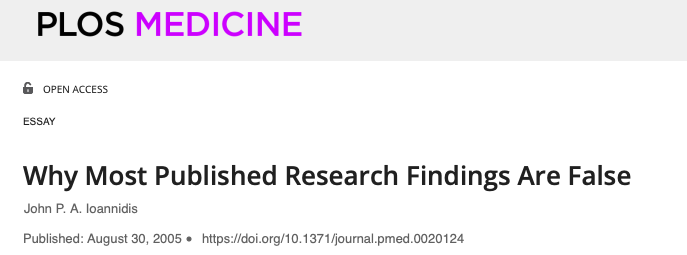
\includegraphics[width=0.75\textwidth,height=\textheight]{../images/ionnidis.png}}

~~

\hypertarget{bishop-2019}{%
\subsubsection*{Bishop (2019)}\label{bishop-2019}}
\addcontentsline{toc}{subsubsection}{Bishop (2019)}

This post by Dorothy Bishop in 2019 nicely captures the situation a number of years later. Clicking on the image below will take you to the paper.

~~

\href{https://www.nature.com/articles/d41586-019-01307-2}{
\includegraphics[width=0.75\textwidth,height=\textheight]{../images/bishop.png}}

\hypertarget{how-to-do-reproducible-research}{%
\subsection{How to do Reproducible Research}\label{how-to-do-reproducible-research}}

One of the biggest challenges facing researchers who are used to the \textbf{old} way of conducting research is that they feel that they don't have the knowledge or technical skills to adopt open and reproducible research practices. But it's not that hard! Before you run your experiment, you can pre-register your hypotheses so that when you come to analyse and write-up your results, you can demonstrate that your predictions really were made in advance of data collection. You can also make your research data open (and \href{https://www.nature.com/articles/sdata201618}{FAIR}) alongside your code so that others can recreate your analyses. And by posting your research article on a pre-print server (such as \href{https://psyarxiv.com}{PsyArXiv} or \href{https://www.biorxiv.org}{bioRxiv}) before submission to a journal, you make your research findings available to all. The adoption of open source software such as R, also means that any research findings you produce can be \emph{re}-produced by others who can access your data and code. This principle of using open tools to allow us to produce open (and reusable) data and code is the fundamental philosophy behind all of the workshops in this unit.

Take the time to read this paper, it's a great guide to the various things you can do to make your own research more open. Just click on the image to open the paper.

\href{https://psycnet.apa.org/fulltext/2019-80290-002.pdf}{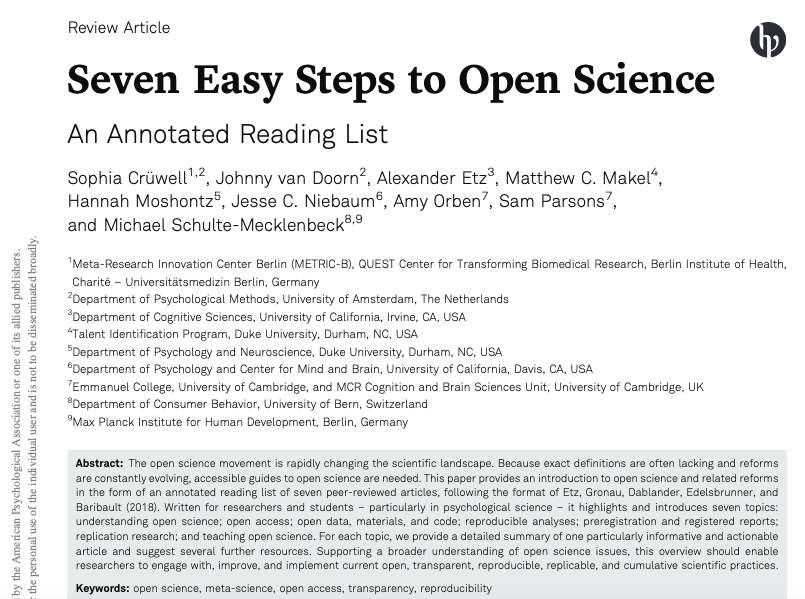
\includegraphics[width=0.75\textwidth,height=\textheight]{../images/7_steps.png}}

~~

\hypertarget{haeffel-2022}{%
\subsubsection*{Haeffel (2022)}\label{haeffel-2022}}
\addcontentsline{toc}{subsubsection}{Haeffel (2022)}

This thought provoking paper by Gerald Haeffel suggests that psychology needs to focus more on theory development (and encourage the publication of results that refute theories).

\href{https://royalsocietypublishing.org/doi/10.1098/rsos.220099}{
\includegraphics[width=0.75\textwidth,height=\textheight]{../images/haeffel.png}}

\hypertarget{experimental-power}{%
\section{Experimental Power}\label{experimental-power}}

We are now going to look at the issues around experimental power (and why it is important). One of the insights revealed by the ``replication crisis'' is that very often research is underpowered for the effect size of interest (i.e., even if the effect is there, your experiment is unlikely to find it). Even when underpowered studies do reveal the effect of interest, the effect size itself will be over-estimated (thus causing problems for future work that might base their power estimates on this incorrect effect size estimate).

One solution to the challenge is to conduct data simulation as part of the experimental design process. There are many ways to do this using R, and there are several packages on CRAN (the Comprehensive R Archive Network) that provide functions to simulate data for different kinds of designs.

~~

~~

If you're interested in reading more about power, you might like to take a look at \href{https://pubmed.ncbi.nlm.nih.gov/19565683/}{this classic ``Power Primer'' paper} by Jacob Cohen.

~~

\hypertarget{open-source-software}{%
\section{Open Source Software}\label{open-source-software}}

If you want to produce open and reproducible research, you should be using open source software in your workflow. Research produced using proprietary software cannot be easily reproduced by others.

Open source software is software that is licensed to be free to modify, remix, and improve. It is usually free to use, and is centred on the principles of open exchange, collaborative participation, rapid prototyping, transparency, meritocracy, and community-oriented development. The move towards open source began in the early 1980s partly because of a \href{https://medium.com/@amogh/the-story-of-open-source-so-far-bfcb685d85a4}{printer} and developed further that decade in the form of the \href{https://en.wikipedia.org/wiki/Free_Software_Foundation}{Free Software Foundation} established by \href{https://en.wikipedia.org/wiki/Richard_Stallman}{Richard Stallman}. In the late 1990s, the \href{https://opensource.org}{Open Source Initiative} was launched to raise awareness and adoption of open source software, and build bridges between open source communities of practice.

Open source software is made by many people and distributed under an OSD-compliant license which grants all the rights to use, study, change, and share the software in modified and unmodified form. Software freedom is essential to enabling community development of open source software.

There is a huge amount of open source software available - some of which you will find useful both in the context of this unit, but also in the context of how you study, and in how you conduct your research.

Below is an interesting CNBC video discussing the rise of Open Source Software - it ends with mention of the need to collaborate in an open manner on global challenges such as the environment, cancer, and Alzheimer's disease.

~~

~~

\hypertarget{statistical-and-scientific-computing}{%
\subsection{Statistical and Scientific Computing}\label{statistical-and-scientific-computing}}

\hypertarget{r-and-rstudio-desktop}{%
\subsubsection*{R and RStudio Desktop}\label{r-and-rstudio-desktop}}
\addcontentsline{toc}{subsubsection}{R and RStudio Desktop}

It goes without saying that R and RStudio Desktop are the two most obvious examples of open source software that are relevant to this course. In terms of other open source languages used for data analysis and statistical modelling, you might also be interested in \href{https://www.python.org}{Python} and \href{https://julialang.org/}{Julia}.

\href{https://www.r-project.org}{
\includegraphics[width=0.15\textwidth,height=\textheight]{../images/r_logo.jpeg}}~~~~~~~~~~~~\href{https://posit.co/products/open-source/rstudio}{
\includegraphics[width=0.25\textwidth,height=\textheight]{../images/RStudio-Logo-Flat.png}}

\hypertarget{python}{%
\subsubsection*{Python}\label{python}}
\addcontentsline{toc}{subsubsection}{Python}

While R tends to be the go-to language for people who are interested in data wrangling, data visualisation, and statistical modelling, Python is arguably the `better' language in the sense it is more general purpose. Python is used widely by the machine learning community (to name just one example).

\href{https://www.python.org}{
\includegraphics[width=0.25\textwidth,height=\textheight]{../images/python-logo-master-v3-TM.png}}

\hypertarget{octave}{%
\subsubsection*{Octave}\label{octave}}
\addcontentsline{toc}{subsubsection}{Octave}

You may have heard of - or even used - MATLAB for numerical computing. There is an open source equivalent, called \href{https://www.gnu.org/software/octave/}{GNU Octave}, that you may be interested in checking out.

\href{https://www.gnu.org/software/octave/}{
\includegraphics[width=0.25\textwidth,height=\textheight]{../images/gnuoctave.jpg}}

\hypertarget{document-creation}{%
\subsection{Document Creation}\label{document-creation}}

Up until this time you've probably mainly used Microsoft Word for writing documents. \href{https://www.libreoffice.org}{LibreOffice} is a great open source equivalent to the Microsoft Office suite and offers a huge range of applications for document writing, working with spreadsheets, and the creation of presentations.

\href{https://www.libreoffice.org}{
\includegraphics[width=0.25\textwidth,height=\textheight]{../images/LibreOffice-6.4.png}}

If you're interested in writing using \href{https://www.markdownguide.org}{Markdown} (which is really easy to get to grips with), you might be interested in using \href{https://opensource.com/article/19/7/enable-collaboration-hackmd}{HackMD}. HackMD is a Markdown editor that critically allows you to write collaborative documents and presentations with others.

\href{https://opensource.com/article/19/7/enable-collaboration-hackmd}{
\includegraphics[width=0.25\textwidth,height=\textheight]{../images/hack_md.png}}

\hypertarget{building-experiments}{%
\subsection{Building Experiments}\label{building-experiments}}

\href{https://www.psychopy.org}{PsychoPy} offers a great open source solution to build experiments to collect human data, and via the companion hosting site \href{https://pavlovia.org}{Pavlovia} provides an easy to use method for running the PsychoPy experiments online. PsychoPy has been around for a number of years and has lots of pre-built experiment templates that you can adapt as needs be. There is a great reference that describes the PsychoPy environment \href{https://link.springer.com/article/10.3758/s13428-018-01193-y}{here}.

\href{https://www.psychopy.org}{
\includegraphics[width=0.25\textwidth,height=\textheight]{../images/psychopyLogoOnlineStrap_h480.png}}~~~~~~~~~~~~\href{https://pavlovia.org}{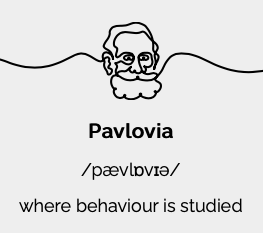
\includegraphics[width=0.25\textwidth,height=\textheight]{../images/pavlovia.png}}

\hypertarget{linux}{%
\subsection{Linux}\label{linux}}

One of the most widely used pieces of open source software is the Linux operating system. Rather than running your computer on Windows, or Mac OS, you could choose to run it using \href{https://www.linux.org}{Linux}. Linux runs the majority of the internet servers in world is becoming increasingly popular in academic settings. Linux refers to a bunch of open source Unix-like operating systems. It was developed and released by \href{https://en.wikipedia.org/wiki/Linus_Torvalds}{Linus Torvalds} in 1991.

\href{https://www.linux.org}{
\includegraphics[width=0.25\textwidth,height=\textheight]{../images/linux.jpg}}

Some of the most popular distributions of Linux are \href{https://ubuntu.com}{Ubuntu}, \href{https://getfedora.org/en/workstation/download/}{Fedora}, and \href{https://www.debian.org}{Debian}. If you really want to get into the computational side of research, it's important to discover the world of Linux.

\href{https://ubuntu.com}{
\includegraphics[width=0.2\textwidth,height=\textheight]{../images/ubuntu-logo112.png}}\href{(https://getfedora.org/en/workstation/download/)}{
\includegraphics[width=0.25\textwidth,height=\textheight]{../images/Fedora-Logo.jpg}}\href{https://www.debian.org}{
\includegraphics[width=0.15\textwidth,height=\textheight]{../images/openlogo.ps.jpg}}

\hypertarget{more-reading}{%
\subsection{More Reading}\label{more-reading}}

If you're interested in other examples of open source software, you might be interested in having a look at this list of open source alternatives on the \href{https://www.techradar.com/uk/best/best-open-source-software}{Tech Radar site}.

\href{https://www.techradar.com/uk/best/best-open-source-software}{
\includegraphics[width=0.75\textwidth,height=\textheight]{../images/oss.png}}

\textbf{End of workshop 1 materials}

\hypertarget{r-and-rstudio}{%
\chapter{R and RStudio}\label{r-and-rstudio}}

\hypertarget{why-r}{%
\section{Why R?}\label{why-r}}

In this workshop we will cover the language, \href{https://www.r-project.org/about.html}{R}, and \href{https://posit.co/products/open-source/rstudio}{RStudio Desktop}, the integrated development environment (IDE) that you will use to write reproducible code involving the wrangling, visualization, summary, and statistical modelling of your data. Both R and RStudio Desktop are examples of \href{https://opensource.com/resources/what-open-source}{Open Source Software}.

The video below introduces you to R and talks about the importance of adopting such tools in our research analysis workflows.

~~

~~

Below is a video of a great talk by J.J. Allaire, entrepreneur and founder of RStudio (and other organizations). This video is from rstudio::conf 2020 and in it J.J. talks about his journey from being a Political Scientist, how he got involved in R, and the importance of Open Source in the context of Reproducible Data Science. If you click on the image, you'll be taken to the RStudio website where you can watch the recording. If you're interested, you might like to look at some of the other videos on the RStudio site.

~~

\href{https://rstudio.com/resources/rstudioconf-2020/open-source-software-for-data-science/}{
\includegraphics{../images/jj_allaire.png}}

~~

\hypertarget{getting-started}{%
\section{Getting Started}\label{getting-started}}

In this next video you'll see how to install R (the language) and RStudio Desktop (the IDE for working with the language). You can download R from \href{https://www.r-project.org}{here} for a variety of platforms including Mac OS, Windows, and Ubuntu. To download free RStudio Desktop just go to \href{https://posit.co}{here}.

If you are using a Chromebook, or have a tablet, or are having difficulties installing R and RStudio Desktop on your computer, you can use \href{https://posit.cloud/plans/free}{Posit cloud} to run the RStudio environment in your browser. You'll need to sign up - there is a free plan available.

~~

~~

\hypertarget{keeping-things-organised}{%
\section{Keeping Things Organised}\label{keeping-things-organised}}

When you are doing data analysis using R, it's important to use a sensible structure for your folders and files. As you saw in the video above, creating a new project with a .Rproj file is the easiest way to this is using RStudio Desktop. Good file management is as important as good coding style (which we'll come to next). There's a great paper on project management that you can read by clicking the image below.

~~

\href{https://journals.plos.org/ploscompbiol/article/file?id=10.1371/journal.pcbi.1005510\&type=printable}{
\includegraphics{../images/wilson_paper.png}}

~~

~~

\hypertarget{good-coding-style}{%
\section{Good Coding Style}\label{good-coding-style}}

In the following video you will learn a little about good coding style. It's important when you're writing analysis scripts that your code is understandable by others, and by future you. If you get into the habit of good coding style early on, it will make things a lot easier in the long run - and you'll find it easier to work collaboratively as others will find it easier to work with you.

~~

~~

You can have a look at the helpful Tidyverse Style Guide \href{https://style.tidyverse.org}{here}.

If you want to make your code and data open (and you really should unless there's a good reason not to do so), it's important to license it properly to allow others to (re)use and remix it. It's often good to use the most permissive license that you can. Some good licenses are the \href{https://opensource.org/licenses/MIT}{MIT License}, and the \href{https://creativecommons.org/licenses/by/4.0/}{Creative Commons License CC-BY 4.0.}

You can use \href{https://choosealicense.com}{this handy guide} if you need help choosing the right license for your own work.

~~

\hypertarget{your-first-r-script}{%
\section{Your First R Script}\label{your-first-r-script}}

You're now going to run your first R script. We will create three visualisations of UFO sightings in the US using a database of more than 80,000 UFO sightings over the years. Before you run the code, you will need to install two packages onto your computer - they are \texttt{tidyverse} and \texttt{patchwork}.

~~

~~

Once you have installed the packages, type the following code into a new R script. Run the code in the same way shown in the video. Does your visualisation look like the one in the video?

\begin{Shaded}
\begin{Highlighting}[]
\FunctionTok{library}\NormalTok{(tidyverse) }\CommentTok{\# load the tidyverse}
\FunctionTok{library}\NormalTok{(patchwork) }\CommentTok{\# needed to combine our 4 plots at the end}
\CommentTok{\# read in data }
\NormalTok{ufo\_sightings }\OtherTok{\textless{}{-}} \FunctionTok{read\_csv}\NormalTok{(}\StringTok{"https://raw.githubusercontent.com/rfordatascience/tidytuesday/master/data/2019/2019{-}06{-}25/ufo\_sightings.csv"}\NormalTok{)}
\CommentTok{\# plot of top 10 US states with number of sightings in each state}
\NormalTok{plot1 }\OtherTok{\textless{}{-}}\NormalTok{ ufo\_sightings }\SpecialCharTok{\%\textgreater{}\%}
  \FunctionTok{filter}\NormalTok{(}\SpecialCharTok{!}\FunctionTok{is.na}\NormalTok{(state)) }\SpecialCharTok{\%\textgreater{}\%}
  \FunctionTok{mutate}\NormalTok{(}\AttributeTok{state =} \FunctionTok{str\_to\_upper}\NormalTok{(state)) }\SpecialCharTok{\%\textgreater{}\%}
  \FunctionTok{group\_by}\NormalTok{(state) }\SpecialCharTok{\%\textgreater{}\%}
  \FunctionTok{tally}\NormalTok{() }\SpecialCharTok{\%\textgreater{}\%}
  \FunctionTok{top\_n}\NormalTok{(}\DecValTok{10}\NormalTok{) }\SpecialCharTok{\%\textgreater{}\%}
  \FunctionTok{ggplot}\NormalTok{(}\FunctionTok{aes}\NormalTok{(}\AttributeTok{x =} \FunctionTok{reorder}\NormalTok{(state, n), }\AttributeTok{y =}\NormalTok{ n, }\AttributeTok{fill =}\NormalTok{ state)) }\SpecialCharTok{+}
  \FunctionTok{geom\_col}\NormalTok{() }\SpecialCharTok{+} 
  \FunctionTok{coord\_flip}\NormalTok{() }\SpecialCharTok{+}
  \FunctionTok{guides}\NormalTok{(}\AttributeTok{fill =} \StringTok{"none"}\NormalTok{) }\SpecialCharTok{+} 
  \FunctionTok{labs}\NormalTok{(}\AttributeTok{title =} \StringTok{"Top 10 States for UFO Sightings"}\NormalTok{,}
       \AttributeTok{x =} \ConstantTok{NULL}\NormalTok{, }
       \AttributeTok{y =} \ConstantTok{NULL}\NormalTok{) }\SpecialCharTok{+}
  \FunctionTok{ylim}\NormalTok{(}\DecValTok{0}\NormalTok{, }\DecValTok{11000}\NormalTok{) }\SpecialCharTok{+}
  \FunctionTok{theme\_minimal}\NormalTok{() }\SpecialCharTok{+}
  \FunctionTok{theme}\NormalTok{(}\AttributeTok{text =} \FunctionTok{element\_text}\NormalTok{(}\AttributeTok{size =} \DecValTok{15}\NormalTok{))}
\CommentTok{\# work out states within lat and long limits (i.e., exclude Alaska)}
\NormalTok{tidied\_ufo }\OtherTok{\textless{}{-}}\NormalTok{ ufo\_sightings }\SpecialCharTok{\%\textgreater{}\%}
  \FunctionTok{filter}\NormalTok{(country }\SpecialCharTok{==} \StringTok{"us"}\NormalTok{) }\SpecialCharTok{\%\textgreater{}\%}
  \FunctionTok{filter}\NormalTok{(latitude }\SpecialCharTok{\textgreater{}} \DecValTok{24} \SpecialCharTok{\&}\NormalTok{ latitude }\SpecialCharTok{\textless{}} \DecValTok{50}\NormalTok{)}
\CommentTok{\# plot all sightings on a map of the US}
\NormalTok{plot2 }\OtherTok{\textless{}{-}}\NormalTok{ tidied\_ufo }\SpecialCharTok{\%\textgreater{}\%}
  \FunctionTok{ggplot}\NormalTok{(}\FunctionTok{aes}\NormalTok{(}\AttributeTok{x =}\NormalTok{ longitude, }\AttributeTok{y =}\NormalTok{ latitude)) }\SpecialCharTok{+} 
  \FunctionTok{geom\_point}\NormalTok{(}\AttributeTok{size =}\NormalTok{ .}\DecValTok{5}\NormalTok{, }\AttributeTok{alpha =}\NormalTok{ .}\DecValTok{25}\NormalTok{) }\SpecialCharTok{+}
  \FunctionTok{theme\_void}\NormalTok{() }\SpecialCharTok{+}
  \FunctionTok{coord\_cartesian}\NormalTok{() }\SpecialCharTok{+}
  \FunctionTok{labs}\NormalTok{(}\AttributeTok{title =} \StringTok{"Sites of UFO Sightings in the US"}\NormalTok{) }\SpecialCharTok{+}
  \FunctionTok{theme}\NormalTok{(}\AttributeTok{text =} \FunctionTok{element\_text}\NormalTok{(}\AttributeTok{size =} \DecValTok{15}\NormalTok{))}
\CommentTok{\# plot of top 10 UFO shapes spotted in California}
\NormalTok{plot3 }\OtherTok{\textless{}{-}}\NormalTok{ tidied\_ufo }\SpecialCharTok{\%\textgreater{}\%}
  \FunctionTok{filter}\NormalTok{(state }\SpecialCharTok{==} \StringTok{"ca"}\NormalTok{) }\SpecialCharTok{\%\textgreater{}\%}
  \FunctionTok{filter}\NormalTok{(ufo\_shape }\SpecialCharTok{!=} \StringTok{"other"}\NormalTok{) }\SpecialCharTok{\%\textgreater{}\%}
  \FunctionTok{filter}\NormalTok{(ufo\_shape }\SpecialCharTok{!=} \StringTok{"unknown"}\NormalTok{) }\SpecialCharTok{\%\textgreater{}\%}
  \FunctionTok{group\_by}\NormalTok{(ufo\_shape) }\SpecialCharTok{\%\textgreater{}\%}
  \FunctionTok{tally}\NormalTok{() }\SpecialCharTok{\%\textgreater{}\%}
  \FunctionTok{top\_n}\NormalTok{(}\DecValTok{10}\NormalTok{) }\SpecialCharTok{\%\textgreater{}\%}
  \FunctionTok{mutate}\NormalTok{(}\AttributeTok{ufo\_shape =} \FunctionTok{str\_to\_title}\NormalTok{(ufo\_shape)) }\SpecialCharTok{\%\textgreater{}\%}
  \FunctionTok{ggplot}\NormalTok{(}\FunctionTok{aes}\NormalTok{(}\AttributeTok{x =} \FunctionTok{reorder}\NormalTok{(ufo\_shape, n), }\AttributeTok{y =}\NormalTok{ n, }\AttributeTok{fill =}\NormalTok{ ufo\_shape)) }\SpecialCharTok{+}
  \FunctionTok{geom\_col}\NormalTok{() }\SpecialCharTok{+} 
  \FunctionTok{coord\_flip}\NormalTok{() }\SpecialCharTok{+}
  \FunctionTok{guides}\NormalTok{(}\AttributeTok{fill =} \StringTok{"none"}\NormalTok{) }\SpecialCharTok{+} 
  \FunctionTok{labs}\NormalTok{(}\AttributeTok{title =} \StringTok{"Top 10 UFO Shapes spotted in California"}\NormalTok{,}
       \AttributeTok{x =} \ConstantTok{NULL}\NormalTok{, }
       \AttributeTok{y =} \ConstantTok{NULL}\NormalTok{) }\SpecialCharTok{+}
  \FunctionTok{theme\_minimal}\NormalTok{() }\SpecialCharTok{+}
  \FunctionTok{theme}\NormalTok{(}\AttributeTok{text =} \FunctionTok{element\_text}\NormalTok{(}\AttributeTok{size =} \DecValTok{15}\NormalTok{))}
\CommentTok{\# Put plots together}
\NormalTok{my\_plot }\OtherTok{\textless{}{-}}\NormalTok{ (plot1 }\SpecialCharTok{+}\NormalTok{ plot3) }\SpecialCharTok{/}\NormalTok{ (plot2)}
\FunctionTok{ggsave}\NormalTok{(}\StringTok{"ufo\_plot.jpg"}\NormalTok{, }\AttributeTok{plot =}\NormalTok{ my\_plot, }\AttributeTok{width =} \DecValTok{12}\NormalTok{, }\AttributeTok{height =} \DecValTok{10}\NormalTok{)}
\end{Highlighting}
\end{Shaded}

{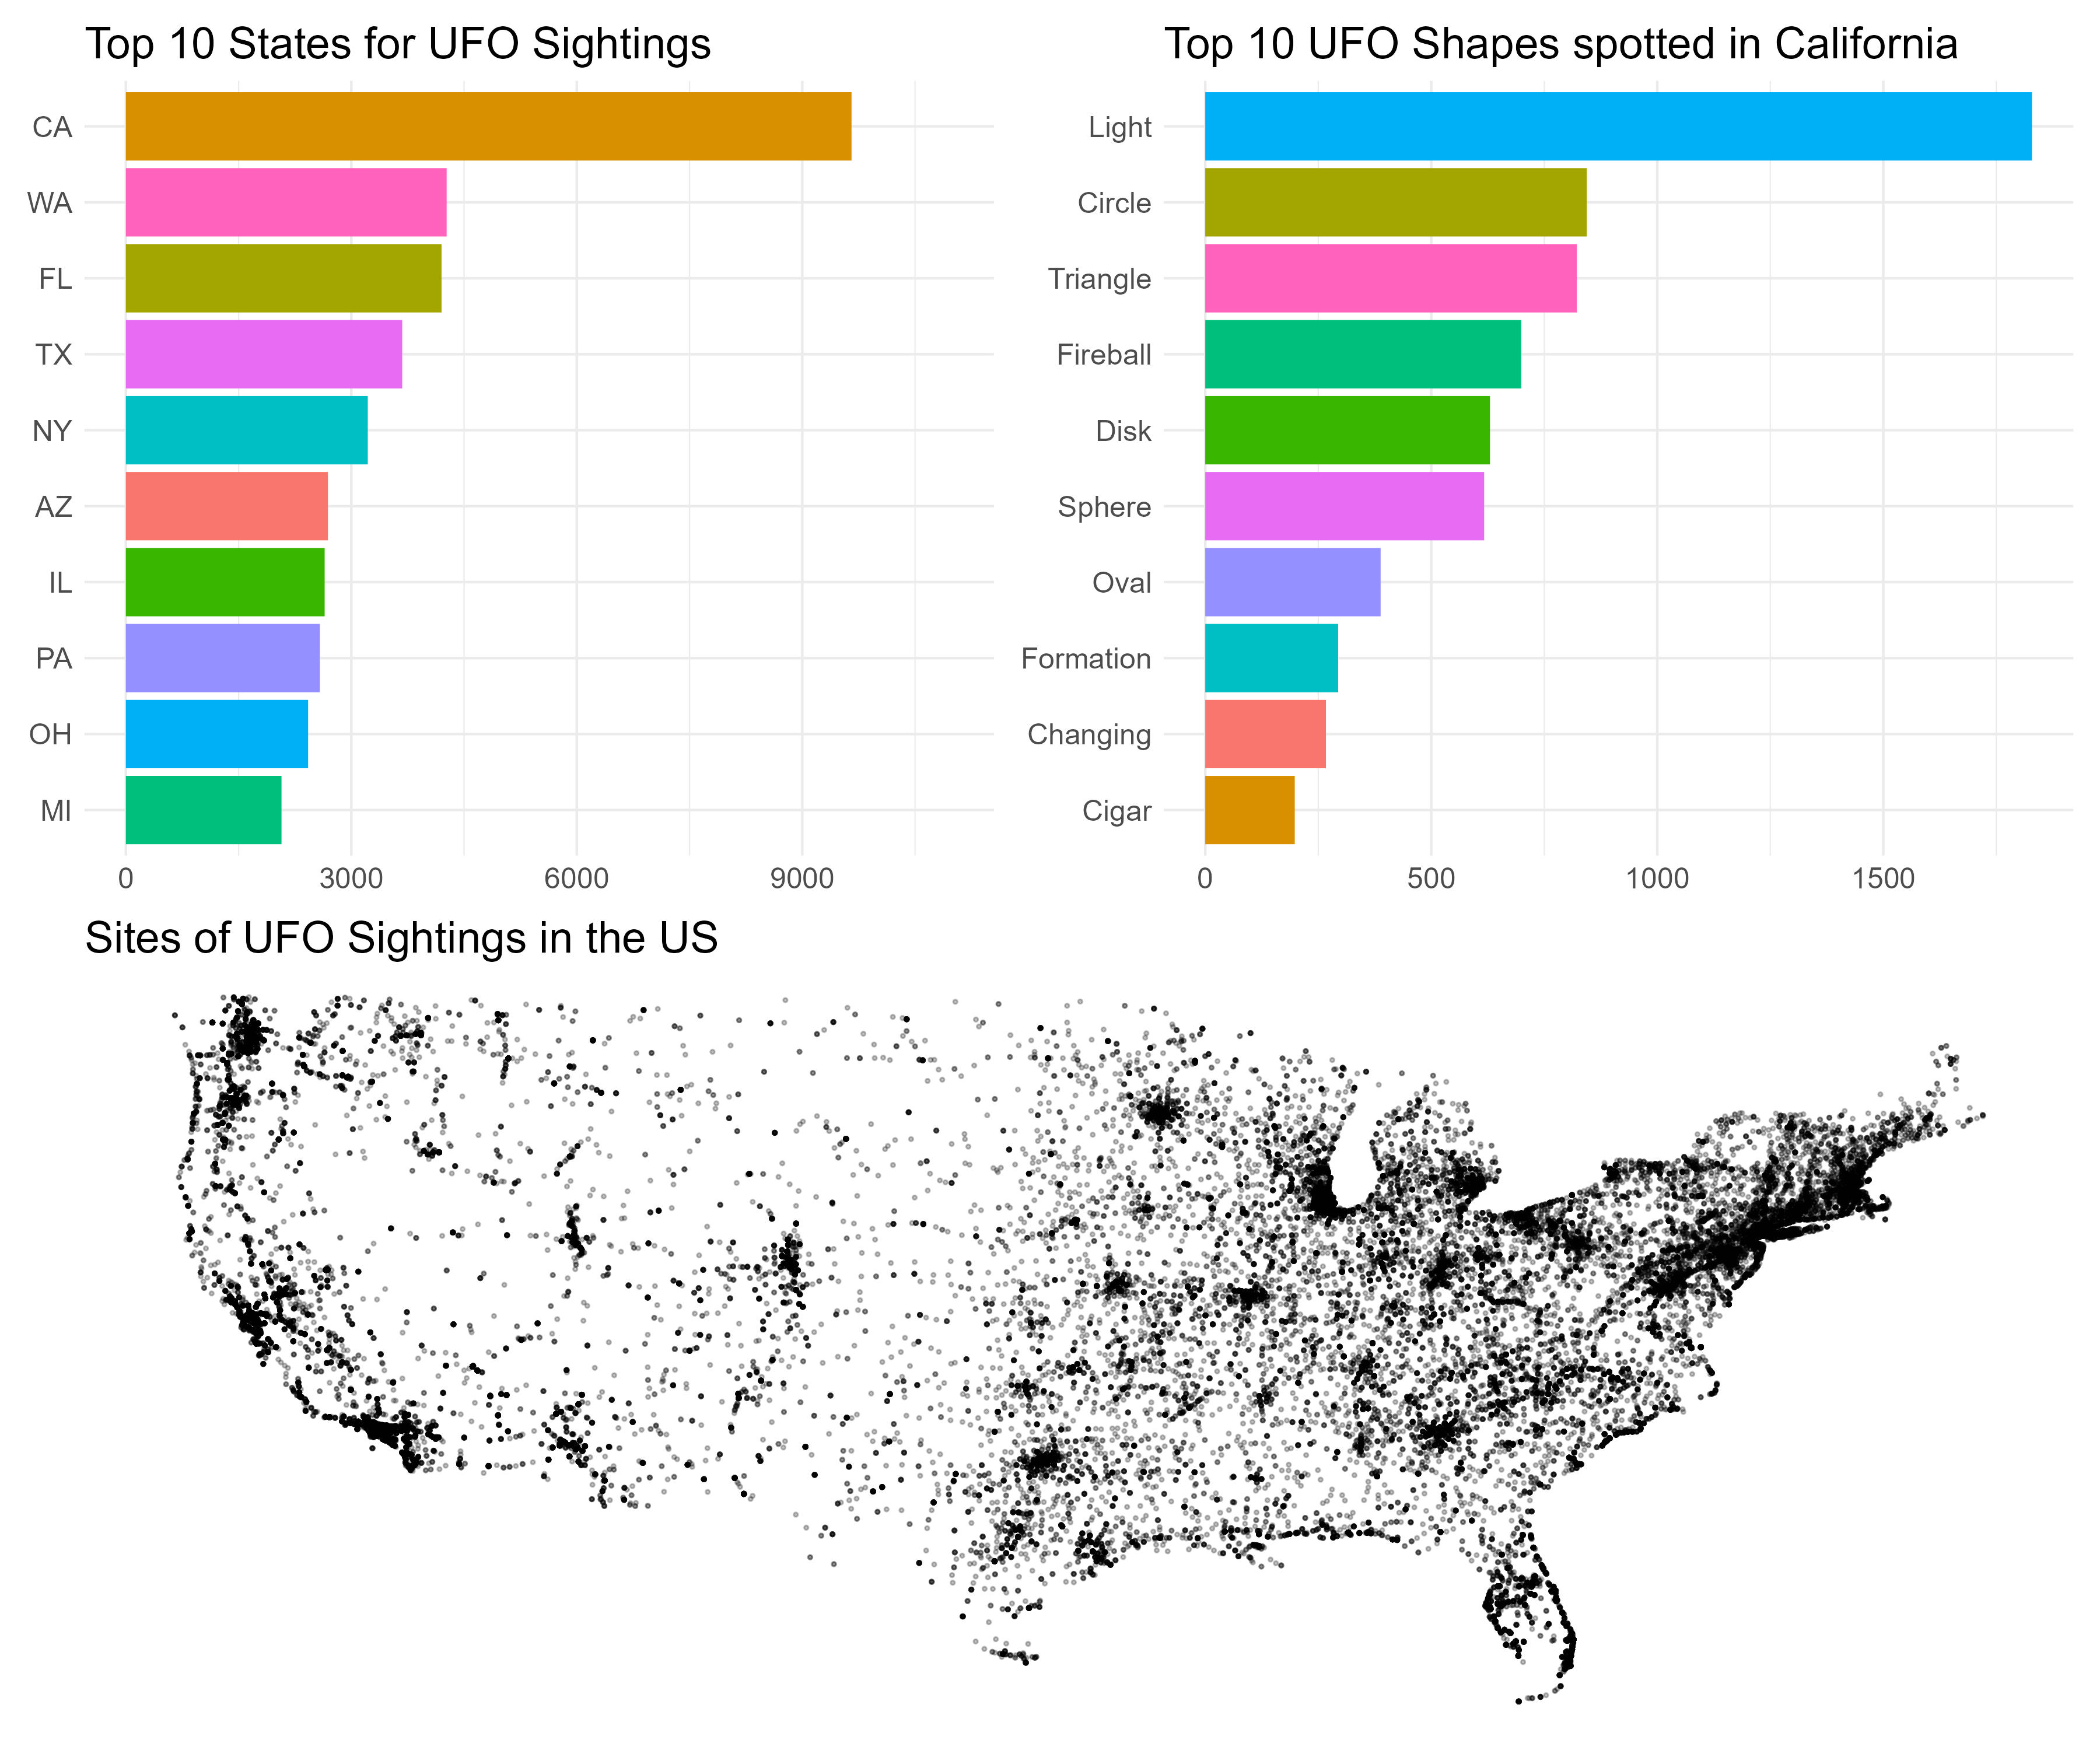
\includegraphics{../images/ufo_plot.jpg}}

\textbf{End of workshop 2 materials}

\hypertarget{data-wrangling-and-data-summarising}{%
\chapter{Data Wrangling and Data Summarising}\label{data-wrangling-and-data-summarising}}

In this workshop we shall take our first look at some key tools in the \href{https://www.tidyverse.org}{Tidyverse} that will allow us to wrangle and tidy our data so that it's in the format that we need in order to visualize and model it. By making our data wrangling reproducible (i.e., by coding it in R), we can easily re-run this stage of our analysis pipeline as new data gets added. Reproducibility of the data wrangling stage is a key part of the analysis process and often gets overlooked in terms of needing to ensure it is reproducible.

The Tidyverse is a collection of packages that all `play nicely' with each other. They are based on a common philosophy where data are represented in rectangular format (i.e., with rows and columns). These rectangular structures are known in the Tidyverse as \texttt{tibbles}. If you're interested, you can read more about \texttt{tibbles} in the R4DS book \href{https://r4ds.had.co.nz/tibbles.html}{here}.

\hypertarget{wrangling-your-data}{%
\section{Wrangling your data}\label{wrangling-your-data}}

Have a look at the following video where I walk you through this worksheet. Then I want you to work through the content by writing (and running) the script on your own machine.

~~

~~

\hypertarget{loading-the-tidyverse}{%
\subsection{Loading the Tidyverse}\label{loading-the-tidyverse}}

Let's take our first look at data wrangling. We are going to start with a dataset that comes with the Tidyverse. The dataset is called \texttt{mpg} and comprises fuel economy data from 1999 to 2008 for 38 popular models of cars in the US.

First, we need to load the \texttt{tidyverse} library with the following:

\begin{Shaded}
\begin{Highlighting}[]
\FunctionTok{library}\NormalTok{(tidyverse)}
\end{Highlighting}
\end{Shaded}

If you run this line without having first installed the Tidyverse on your computer, you will encounter an error. R packages only need to be installed once, so if you want to load one into your library for the first time, you need to install it with \texttt{install.packages(*packagename*)}.

For the \texttt{tidyverse} we need to install it with:

\begin{Shaded}
\begin{Highlighting}[]
\FunctionTok{install.packages}\NormalTok{(}\StringTok{"tidyverse"}\NormalTok{)}
\end{Highlighting}
\end{Shaded}

Once you have installed the \texttt{tidyverse}, you can then load it into your llbrary with the \texttt{library()} function. You only ever need to install a package once on your machine (unless you have updated R or you want to install the most up-to-date version of a particular package). When you are writing your R scripts, you never want to have the \texttt{install.packages()} function in the body of the script as if someone else were to run your script, this would update packages on their computer (which they might not want).

\hypertarget{the-mpg-dataset}{%
\subsubsection*{\texorpdfstring{The \texttt{mpg} dataset}{The mpg dataset}}\label{the-mpg-dataset}}
\addcontentsline{toc}{subsubsection}{The \texttt{mpg} dataset}

The \texttt{mpg} dataset is loaded as part of the Tidyverse. In the help file, which you can access by typing \texttt{help(mpg)} or \texttt{?mpg} we see the following:

Description This dataset contains a subset of the fuel economy data that the EPA makes available on \url{http://fueleconomy.gov}. It contains only models which had a new release every year between 1999 and 2008 - this was used as a proxy for the popularity of the car.

A data frame with 234 rows and 11 variables.

manufacturer - manufacturer model - model name displ - engine displacement, in litres year - year of manufacture cyl - number of cylinders trans -type of transmission drv -f = front-wheel drive, r = rear wheel drive, 4 = 4wd cty - city miles per gallon hwy - highway miles per gallon fl - fuel type class - ``type'' of car

Note you can also use help to inspect functions, for example: Typing \texttt{?sd} will show you the documentation for R's Standard Deviation function.

\hypertarget{using-head-and-str}{%
\subsection{\texorpdfstring{Using \texttt{head()} and \texttt{str()}}{Using head() and str()}}\label{using-head-and-str}}

We can explore the \texttt{mpg} dataset that is loaded with the Tidyverse in a number of ways. If we want to look at the first 6 lines of the dataset, we can use the \texttt{head()} function.

\begin{Shaded}
\begin{Highlighting}[]
\FunctionTok{head}\NormalTok{(mpg)}
\end{Highlighting}
\end{Shaded}

\begin{verbatim}
## # A tibble: 6 x 11
##   manufacturer model displ  year   cyl trans      drv     cty   hwy fl    class 
##   <chr>        <chr> <dbl> <int> <int> <chr>      <chr> <int> <int> <chr> <chr> 
## 1 audi         a4      1.8  1999     4 auto(l5)   f        18    29 p     compa~
## 2 audi         a4      1.8  1999     4 manual(m5) f        21    29 p     compa~
## 3 audi         a4      2    2008     4 manual(m6) f        20    31 p     compa~
## 4 audi         a4      2    2008     4 auto(av)   f        21    30 p     compa~
## 5 audi         a4      2.8  1999     6 auto(l5)   f        16    26 p     compa~
## 6 audi         a4      2.8  1999     6 manual(m5) f        18    26 p     compa~
\end{verbatim}

We see that it is a tibble - or a rectangular data frame - made up of rows and columns. This is \texttt{tidy} format where each observation corresponds to a row. Most of the analyses we will run in R involve \texttt{tidy} data. Within the Tidyverse, the \texttt{tibble} is the standard way to represent data. You'll spend a lot of time tidying and wrangling your data to get it into this format! By doing this in R using a script that you write, you are making this key stage \emph{reproducible}. You can run the script again on an updated or different dataset - thus likely saving you lots of time!

We can also ask for information about the structure of our dataset with \texttt{str()}. This will tell us about the columns, what type of variable each is, the number of rows etc.

\begin{Shaded}
\begin{Highlighting}[]
\FunctionTok{str}\NormalTok{(mpg)}
\end{Highlighting}
\end{Shaded}

\begin{verbatim}
## tibble [234 x 11] (S3: tbl_df/tbl/data.frame)
##  $ manufacturer: chr [1:234] "audi" "audi" "audi" "audi" ...
##  $ model       : chr [1:234] "a4" "a4" "a4" "a4" ...
##  $ displ       : num [1:234] 1.8 1.8 2 2 2.8 2.8 3.1 1.8 1.8 2 ...
##  $ year        : int [1:234] 1999 1999 2008 2008 1999 1999 2008 1999 1999 2008 ...
##  $ cyl         : int [1:234] 4 4 4 4 6 6 6 4 4 4 ...
##  $ trans       : chr [1:234] "auto(l5)" "manual(m5)" "manual(m6)" "auto(av)" ...
##  $ drv         : chr [1:234] "f" "f" "f" "f" ...
##  $ cty         : int [1:234] 18 21 20 21 16 18 18 18 16 20 ...
##  $ hwy         : int [1:234] 29 29 31 30 26 26 27 26 25 28 ...
##  $ fl          : chr [1:234] "p" "p" "p" "p" ...
##  $ class       : chr [1:234] "compact" "compact" "compact" "compact" ...
\end{verbatim}

\hypertarget{use-select-to-select-columns}{%
\subsection{\texorpdfstring{Use \texttt{select()} to select columns}{Use select() to select columns}}\label{use-select-to-select-columns}}

If we want to, we could just select one of the columns using the \texttt{select()} function. Below we are just selecing the column entitled \texttt{manufacturer}.

\begin{Shaded}
\begin{Highlighting}[]
\NormalTok{mpg }\SpecialCharTok{\%\textgreater{}\%}
  \FunctionTok{select}\NormalTok{(manufacturer)}
\end{Highlighting}
\end{Shaded}

\begin{verbatim}
## # A tibble: 234 x 1
##    manufacturer
##    <chr>       
##  1 audi        
##  2 audi        
##  3 audi        
##  4 audi        
##  5 audi        
##  6 audi        
##  7 audi        
##  8 audi        
##  9 audi        
## 10 audi        
## # i 224 more rows
\end{verbatim}

Related to the \texttt{select()} function is \texttt{rename()}. It does exactly what you think it might; it renames a column.

We can also look at the different car manufacturers in the dataset by using the \texttt{distinct()} function. This gives us the unique manufacturer names. This function can be quite handy if you want to check a dataset for duplicates of (e.g.) participant IDs.

\begin{Shaded}
\begin{Highlighting}[]
\NormalTok{mpg }\SpecialCharTok{\%\textgreater{}\%}
  \FunctionTok{distinct}\NormalTok{(manufacturer)}
\end{Highlighting}
\end{Shaded}

\begin{verbatim}
## # A tibble: 15 x 1
##    manufacturer
##    <chr>       
##  1 audi        
##  2 chevrolet   
##  3 dodge       
##  4 ford        
##  5 honda       
##  6 hyundai     
##  7 jeep        
##  8 land rover  
##  9 lincoln     
## 10 mercury     
## 11 nissan      
## 12 pontiac     
## 13 subaru      
## 14 toyota      
## 15 volkswagen
\end{verbatim}

\hypertarget{use-filter-to-select-rows}{%
\subsection{\texorpdfstring{Use \texttt{filter()} to select rows}{Use filter() to select rows}}\label{use-filter-to-select-rows}}

Sometimes we might want to select only a subset of rows in our dataset. We can do that using the \texttt{filter()} function. For example, here we filter our dataset to include only cars made by `honda'.

\begin{Shaded}
\begin{Highlighting}[]
\NormalTok{mpg }\SpecialCharTok{\%\textgreater{}\%}
  \FunctionTok{filter}\NormalTok{(manufacturer }\SpecialCharTok{==} \StringTok{"honda"}\NormalTok{)}
\end{Highlighting}
\end{Shaded}

\begin{verbatim}
## # A tibble: 9 x 11
##   manufacturer model displ  year   cyl trans      drv     cty   hwy fl    class 
##   <chr>        <chr> <dbl> <int> <int> <chr>      <chr> <int> <int> <chr> <chr> 
## 1 honda        civic   1.6  1999     4 manual(m5) f        28    33 r     subco~
## 2 honda        civic   1.6  1999     4 auto(l4)   f        24    32 r     subco~
## 3 honda        civic   1.6  1999     4 manual(m5) f        25    32 r     subco~
## 4 honda        civic   1.6  1999     4 manual(m5) f        23    29 p     subco~
## 5 honda        civic   1.6  1999     4 auto(l4)   f        24    32 r     subco~
## 6 honda        civic   1.8  2008     4 manual(m5) f        26    34 r     subco~
## 7 honda        civic   1.8  2008     4 auto(l5)   f        25    36 r     subco~
## 8 honda        civic   1.8  2008     4 auto(l5)   f        24    36 c     subco~
## 9 honda        civic   2    2008     4 manual(m6) f        21    29 p     subco~
\end{verbatim}

Note, we use the operator \texttt{==} which means `is equal to'. This is a logical operator - other logical operators include less than \texttt{\textless{}}, greater than \texttt{\textgreater{}}, less than or equal to \texttt{\textless{}=}, greater then or equal to \texttt{\textgreater{}=}, and is not equal to \texttt{!=}.

We can also filter using a combination of possibilities via logical OR \texttt{\textbar{}} or logical AND \texttt{\&}. The first code chunk below filters the dataset for cases where the manufacturer is `honda' OR `toyota'.

\begin{Shaded}
\begin{Highlighting}[]
\NormalTok{mpg }\SpecialCharTok{\%\textgreater{}\%}
  \FunctionTok{filter}\NormalTok{(manufacturer }\SpecialCharTok{==} \StringTok{"honda"} \SpecialCharTok{|}\NormalTok{ manufacturer }\SpecialCharTok{==} \StringTok{"toyota"}\NormalTok{)}
\end{Highlighting}
\end{Shaded}

\begin{verbatim}
## # A tibble: 43 x 11
##    manufacturer model      displ  year   cyl trans drv     cty   hwy fl    class
##    <chr>        <chr>      <dbl> <int> <int> <chr> <chr> <int> <int> <chr> <chr>
##  1 honda        civic        1.6  1999     4 manu~ f        28    33 r     subc~
##  2 honda        civic        1.6  1999     4 auto~ f        24    32 r     subc~
##  3 honda        civic        1.6  1999     4 manu~ f        25    32 r     subc~
##  4 honda        civic        1.6  1999     4 manu~ f        23    29 p     subc~
##  5 honda        civic        1.6  1999     4 auto~ f        24    32 r     subc~
##  6 honda        civic        1.8  2008     4 manu~ f        26    34 r     subc~
##  7 honda        civic        1.8  2008     4 auto~ f        25    36 r     subc~
##  8 honda        civic        1.8  2008     4 auto~ f        24    36 c     subc~
##  9 honda        civic        2    2008     4 manu~ f        21    29 p     subc~
## 10 toyota       4runner 4~   2.7  1999     4 manu~ 4        15    20 r     suv  
## # i 33 more rows
\end{verbatim}

While below we filter for cases where the manufacturer is `honda' and the year of manufacture is `1999'.

\begin{Shaded}
\begin{Highlighting}[]
\NormalTok{mpg }\SpecialCharTok{\%\textgreater{}\%} 
  \FunctionTok{filter}\NormalTok{(manufacturer }\SpecialCharTok{==} \StringTok{"honda"} \SpecialCharTok{\&}\NormalTok{ year }\SpecialCharTok{==} \StringTok{"1999"}\NormalTok{)}
\end{Highlighting}
\end{Shaded}

\begin{verbatim}
## # A tibble: 5 x 11
##   manufacturer model displ  year   cyl trans      drv     cty   hwy fl    class 
##   <chr>        <chr> <dbl> <int> <int> <chr>      <chr> <int> <int> <chr> <chr> 
## 1 honda        civic   1.6  1999     4 manual(m5) f        28    33 r     subco~
## 2 honda        civic   1.6  1999     4 auto(l4)   f        24    32 r     subco~
## 3 honda        civic   1.6  1999     4 manual(m5) f        25    32 r     subco~
## 4 honda        civic   1.6  1999     4 manual(m5) f        23    29 p     subco~
## 5 honda        civic   1.6  1999     4 auto(l4)   f        24    32 r     subco~
\end{verbatim}

\hypertarget{combining-functions}{%
\subsubsection*{Combining functions}\label{combining-functions}}
\addcontentsline{toc}{subsubsection}{Combining functions}

We can combine the use of \texttt{filter()} with \texttt{select()} to filter for case where the manufacturer is `honda', the year of manufacture is `1999' and we only want to display these two columns plus those telling us about fuel economy - \texttt{cty} and \texttt{hwy}.

\begin{Shaded}
\begin{Highlighting}[]
\NormalTok{mpg }\SpecialCharTok{\%\textgreater{}\%} 
  \FunctionTok{filter}\NormalTok{(manufacturer }\SpecialCharTok{==} \StringTok{"honda"} \SpecialCharTok{\&}\NormalTok{ year }\SpecialCharTok{==} \StringTok{"1999"}\NormalTok{) }\SpecialCharTok{\%\textgreater{}\%}
  \FunctionTok{select}\NormalTok{(manufacturer, year, cty, hwy)}
\end{Highlighting}
\end{Shaded}

\begin{verbatim}
## # A tibble: 5 x 4
##   manufacturer  year   cty   hwy
##   <chr>        <int> <int> <int>
## 1 honda         1999    28    33
## 2 honda         1999    24    32
## 3 honda         1999    25    32
## 4 honda         1999    23    29
## 5 honda         1999    24    32
\end{verbatim}

By combining just a few functions, you can imagine that we can build some quite complex data wrangling rules quite straightforwardly.

\hypertarget{the-pipe}{%
\subsection{\texorpdfstring{The pipe \texttt{\%\textgreater{}\%}}{The pipe \%\textgreater\%}}\label{the-pipe}}

Note that in these examples above we used the \texttt{\%\textgreater{}\%} operator - this is called the pipe and allows us to pass information from one side of the pipe to the other. You can read it out load as `and then'. All of the functions (such as \texttt{select()}, \texttt{filter()} etc.) in the Tidyverse are known as verbs, and they describe what they do. The pipe is one of the most commonly used operators in the Tidyverse and allows us to chain together different lines of code - with the output of each line being passed on as input into the next. In this example, the dataset \texttt{mpg} is passed along to the \texttt{distinct()} function where we ask for a list of the distinct (i.e., unique) manufacturers. This output itself is a vector. Vectors are a basic data structure and contain elements of the same type - for example, a bunch of numbers. We can add another line to our piped chain to tell us how many elements are in this vector. We could read this out loud as `take the dataset mpg, and then work out the distinct manufacturer names, and then count them'.

\begin{Shaded}
\begin{Highlighting}[]
\NormalTok{mpg }\SpecialCharTok{\%\textgreater{}\%} 
  \FunctionTok{distinct}\NormalTok{(manufacturer) }\SpecialCharTok{\%\textgreater{}\%}
  \FunctionTok{count}\NormalTok{()}
\end{Highlighting}
\end{Shaded}

\begin{verbatim}
## # A tibble: 1 x 1
##       n
##   <int>
## 1    15
\end{verbatim}

\hypertarget{tidying-up-a-dataset}{%
\subsection{Tidying up a dataset}\label{tidying-up-a-dataset}}

\hypertarget{tidying-variable-names}{%
\subsubsection*{Tidying variable names}\label{tidying-variable-names}}
\addcontentsline{toc}{subsubsection}{Tidying variable names}

At the moment, the car manufacturer names are all in lower case. It would look a lot nicer if they were in title case (i.e., with capitalisation on the first letter of each word). We can use the \texttt{mutate()} function to create a new column - this time, the name of the new column is also the name of the old column that we're wanting to modify using the function \texttt{str\_to\_title()}. What this will do is overwrite the column \texttt{manufacturer} and replace it with the new version with the car manufacturer names in title case.

\begin{Shaded}
\begin{Highlighting}[]
\NormalTok{mpg }\SpecialCharTok{\%\textgreater{}\%}
  \FunctionTok{mutate}\NormalTok{(}\AttributeTok{manufacturer =} \FunctionTok{str\_to\_title}\NormalTok{(manufacturer)) }
\end{Highlighting}
\end{Shaded}

\begin{verbatim}
## # A tibble: 234 x 11
##    manufacturer model      displ  year   cyl trans drv     cty   hwy fl    class
##    <chr>        <chr>      <dbl> <int> <int> <chr> <chr> <int> <int> <chr> <chr>
##  1 Audi         a4           1.8  1999     4 auto~ f        18    29 p     comp~
##  2 Audi         a4           1.8  1999     4 manu~ f        21    29 p     comp~
##  3 Audi         a4           2    2008     4 manu~ f        20    31 p     comp~
##  4 Audi         a4           2    2008     4 auto~ f        21    30 p     comp~
##  5 Audi         a4           2.8  1999     6 auto~ f        16    26 p     comp~
##  6 Audi         a4           2.8  1999     6 manu~ f        18    26 p     comp~
##  7 Audi         a4           3.1  2008     6 auto~ f        18    27 p     comp~
##  8 Audi         a4 quattro   1.8  1999     4 manu~ 4        18    26 p     comp~
##  9 Audi         a4 quattro   1.8  1999     4 auto~ 4        16    25 p     comp~
## 10 Audi         a4 quattro   2    2008     4 manu~ 4        20    28 p     comp~
## # i 224 more rows
\end{verbatim}

The column \texttt{model} is also lowercase. Let's make that title case too. We can use the \texttt{mutate()} function to work over more than one column at the same time like this:

\begin{Shaded}
\begin{Highlighting}[]
\NormalTok{mpg }\SpecialCharTok{\%\textgreater{}\%}
  \FunctionTok{mutate}\NormalTok{(}\AttributeTok{manufacturer =} \FunctionTok{str\_to\_title}\NormalTok{(manufacturer), }\AttributeTok{model =} \FunctionTok{str\_to\_title}\NormalTok{(model))}
\end{Highlighting}
\end{Shaded}

\begin{verbatim}
## # A tibble: 234 x 11
##    manufacturer model      displ  year   cyl trans drv     cty   hwy fl    class
##    <chr>        <chr>      <dbl> <int> <int> <chr> <chr> <int> <int> <chr> <chr>
##  1 Audi         A4           1.8  1999     4 auto~ f        18    29 p     comp~
##  2 Audi         A4           1.8  1999     4 manu~ f        21    29 p     comp~
##  3 Audi         A4           2    2008     4 manu~ f        20    31 p     comp~
##  4 Audi         A4           2    2008     4 auto~ f        21    30 p     comp~
##  5 Audi         A4           2.8  1999     6 auto~ f        16    26 p     comp~
##  6 Audi         A4           2.8  1999     6 manu~ f        18    26 p     comp~
##  7 Audi         A4           3.1  2008     6 auto~ f        18    27 p     comp~
##  8 Audi         A4 Quattro   1.8  1999     4 manu~ 4        18    26 p     comp~
##  9 Audi         A4 Quattro   1.8  1999     4 auto~ 4        16    25 p     comp~
## 10 Audi         A4 Quattro   2    2008     4 manu~ 4        20    28 p     comp~
## # i 224 more rows
\end{verbatim}

There are quite a few columns there, so how about we select just the manufacturer, model, year, transmission, and hwy columns:

\begin{Shaded}
\begin{Highlighting}[]
\NormalTok{mpg }\SpecialCharTok{\%\textgreater{}\%}
  \FunctionTok{mutate}\NormalTok{(}\AttributeTok{manufacturer =} \FunctionTok{str\_to\_title}\NormalTok{(manufacturer), }\AttributeTok{model =} \FunctionTok{str\_to\_title}\NormalTok{(model)) }\SpecialCharTok{\%\textgreater{}\%}
  \FunctionTok{select}\NormalTok{(manufacturer, model, year, trans, hwy)}
\end{Highlighting}
\end{Shaded}

\begin{verbatim}
## # A tibble: 234 x 5
##    manufacturer model       year trans        hwy
##    <chr>        <chr>      <int> <chr>      <int>
##  1 Audi         A4          1999 auto(l5)      29
##  2 Audi         A4          1999 manual(m5)    29
##  3 Audi         A4          2008 manual(m6)    31
##  4 Audi         A4          2008 auto(av)      30
##  5 Audi         A4          1999 auto(l5)      26
##  6 Audi         A4          1999 manual(m5)    26
##  7 Audi         A4          2008 auto(av)      27
##  8 Audi         A4 Quattro  1999 manual(m5)    26
##  9 Audi         A4 Quattro  1999 auto(l5)      25
## 10 Audi         A4 Quattro  2008 manual(m6)    28
## # i 224 more rows
\end{verbatim}

\hypertarget{recoding-variables}{%
\subsubsection*{Recoding variables}\label{recoding-variables}}
\addcontentsline{toc}{subsubsection}{Recoding variables}

In the real world, data frames do not always arrive on our computer in tidy format. Very often you need to engage in some data tidying before you can do anything useful with them. We're going to look at an example of how we go from messy data to tidy data.

\begin{Shaded}
\begin{Highlighting}[]
\NormalTok{my\_messy\_data }\OtherTok{\textless{}{-}} \FunctionTok{read\_csv}\NormalTok{(}\StringTok{"https://raw.githubusercontent.com/ajstewartlang/03\_data\_wrangling/master/data/my\_data.csv"}\NormalTok{)}
\end{Highlighting}
\end{Shaded}

We ran a reaction time experiment with 24 participants and 4 conditions - they are numbered 1-4 in our data file.

\begin{Shaded}
\begin{Highlighting}[]
\FunctionTok{head}\NormalTok{(my\_messy\_data)}
\end{Highlighting}
\end{Shaded}

\begin{verbatim}
## # A tibble: 6 x 3
##   participant condition    rt
##         <dbl>     <dbl> <dbl>
## 1           1         1   879
## 2           1         2  1027
## 3           1         3  1108
## 4           1         4   765
## 5           2         1  1042
## 6           2         2  1050
\end{verbatim}

This is a repeated measures design where we had one factor (Prime Type) with two levels (A vs.~B) and a second factor (Target Type) with two levels (A vs.~B). We want to recode our data frame so it better matches our experimental design. First we need to recode our 4 conditions like this:

Recode condition columns follows: Condition 1 = Prime A, Target A Condition 2 = Prime A, Target B Condition 3 = Prime B, Target A Condition 4 = Prime B, Target B

\begin{Shaded}
\begin{Highlighting}[]
\NormalTok{my\_messy\_data }\SpecialCharTok{\%\textgreater{}\%} 
  \FunctionTok{mutate}\NormalTok{(}\AttributeTok{condition =} \FunctionTok{recode}\NormalTok{(condition,}
                            \StringTok{"1"} \OtherTok{=} \StringTok{"PrimeA\_TargetA"}\NormalTok{,}
                            \StringTok{"2"} \OtherTok{=} \StringTok{"PrimeA\_TargetB"}\NormalTok{, }
                            \StringTok{"3"} \OtherTok{=} \StringTok{"PrimeB\_TargetA"}\NormalTok{, }
                            \StringTok{"4"} \OtherTok{=} \StringTok{"PrimeB\_TargetB"}\NormalTok{)) }\SpecialCharTok{\%\textgreater{}\%}
  \FunctionTok{head}\NormalTok{()}
\end{Highlighting}
\end{Shaded}

\begin{verbatim}
## # A tibble: 6 x 3
##   participant condition         rt
##         <dbl> <chr>          <dbl>
## 1           1 PrimeA_TargetA   879
## 2           1 PrimeA_TargetB  1027
## 3           1 PrimeB_TargetA  1108
## 4           1 PrimeB_TargetB   765
## 5           2 PrimeA_TargetA  1042
## 6           2 PrimeA_TargetB  1050
\end{verbatim}

We now need to separate out our Condition column into two - one for our first factor (Prime), and one for our second factor (Target). The \texttt{separate()} function does just this - when used in conjunction with a piped tibble, it needs to know which column we want to separate, what new columns to create by separating that original column, and on what basis we want to do the separation. In the example below we tell \texttt{separate()} that we want to separate the column labeled \texttt{condition} into two new columns called \texttt{Prime} and \texttt{Target} and we want to do this at any points where a \texttt{\_} is present in the column to be separated.

\begin{Shaded}
\begin{Highlighting}[]
\NormalTok{my\_messy\_data }\SpecialCharTok{\%\textgreater{}\%} 
  \FunctionTok{mutate}\NormalTok{(}\AttributeTok{condition =} \FunctionTok{recode}\NormalTok{(condition,}
                            \StringTok{"1"} \OtherTok{=} \StringTok{"PrimeA\_TargetA"}\NormalTok{,}
                            \StringTok{"2"} \OtherTok{=} \StringTok{"PrimeA\_TargetB"}\NormalTok{, }
                            \StringTok{"3"} \OtherTok{=} \StringTok{"PrimeB\_TargetA"}\NormalTok{, }
                            \StringTok{"4"} \OtherTok{=} \StringTok{"PrimeB\_TargetB"}\NormalTok{)) }\SpecialCharTok{\%\textgreater{}\%}
  \FunctionTok{separate}\NormalTok{(}\AttributeTok{col =} \StringTok{"condition"}\NormalTok{, }\AttributeTok{into =} \FunctionTok{c}\NormalTok{(}\StringTok{"Prime"}\NormalTok{, }\StringTok{"Target"}\NormalTok{), }\AttributeTok{sep =} \StringTok{"\_"}\NormalTok{)}
\end{Highlighting}
\end{Shaded}

\begin{verbatim}
## # A tibble: 96 x 4
##    participant Prime  Target     rt
##          <dbl> <chr>  <chr>   <dbl>
##  1           1 PrimeA TargetA   879
##  2           1 PrimeA TargetB  1027
##  3           1 PrimeB TargetA  1108
##  4           1 PrimeB TargetB   765
##  5           2 PrimeA TargetA  1042
##  6           2 PrimeA TargetB  1050
##  7           2 PrimeB TargetA   942
##  8           2 PrimeB TargetB   945
##  9           3 PrimeA TargetA   943
## 10           3 PrimeA TargetB   910
## # i 86 more rows
\end{verbatim}

\begin{Shaded}
\begin{Highlighting}[]
\NormalTok{my\_messy\_data }\SpecialCharTok{\%\textgreater{}\%} 
  \FunctionTok{mutate}\NormalTok{(}\AttributeTok{condition =} \FunctionTok{recode}\NormalTok{(condition,}
                            \StringTok{"1"} \OtherTok{=} \StringTok{"PrimeA\_TargetA"}\NormalTok{,}
                            \StringTok{"2"} \OtherTok{=} \StringTok{"PrimeA\_TargetB"}\NormalTok{, }
                            \StringTok{"3"} \OtherTok{=} \StringTok{"PrimeB\_TargetA"}\NormalTok{, }
                            \StringTok{"4"} \OtherTok{=} \StringTok{"PrimeB\_TargetB"}\NormalTok{)) }\SpecialCharTok{\%\textgreater{}\%}
  \FunctionTok{separate}\NormalTok{(}\AttributeTok{col =} \StringTok{"condition"}\NormalTok{, }\AttributeTok{into =} \FunctionTok{c}\NormalTok{(}\StringTok{"Prime"}\NormalTok{, }\StringTok{"Target"}\NormalTok{), }\AttributeTok{sep =} \StringTok{"\_"}\NormalTok{) }\SpecialCharTok{\%\textgreater{}\%}
  \FunctionTok{mutate}\NormalTok{(}\AttributeTok{Prime =} \FunctionTok{factor}\NormalTok{(Prime), }\AttributeTok{Target =} \FunctionTok{factor}\NormalTok{(Target))}
\end{Highlighting}
\end{Shaded}

\begin{verbatim}
## # A tibble: 96 x 4
##    participant Prime  Target     rt
##          <dbl> <fct>  <fct>   <dbl>
##  1           1 PrimeA TargetA   879
##  2           1 PrimeA TargetB  1027
##  3           1 PrimeB TargetA  1108
##  4           1 PrimeB TargetB   765
##  5           2 PrimeA TargetA  1042
##  6           2 PrimeA TargetB  1050
##  7           2 PrimeB TargetA   942
##  8           2 PrimeB TargetB   945
##  9           3 PrimeA TargetA   943
## 10           3 PrimeA TargetB   910
## # i 86 more rows
\end{verbatim}

\hypertarget{the-pivot-functions}{%
\subsubsection*{The pivot functions}\label{the-pivot-functions}}
\addcontentsline{toc}{subsubsection}{The pivot functions}

Most of the analysis we will conduct in R requires our data to be in tidy, or long, format. In such data sets, one row corresponds to one observation. In the real world, data are rarely in the right format for analysis. In R, the \texttt{pivot\_wider()} and \texttt{pivot\_longer()} functions are designed to reshape our data files. First, let's load a datafile that is in wide format (i.e., multiple observations per row). It is from an experiment where we had four conditions (labelled Condition1, Condition2, Condition3, and Condition4). In addition to there being a column for each of the 4 conditions, we also have a column corresponding to participant ID. Each cell in the data set corresponds to a reaction time (measured in milliseconds).

\begin{Shaded}
\begin{Highlighting}[]
\NormalTok{my\_wide\_data }\OtherTok{\textless{}{-}} \FunctionTok{read\_csv}\NormalTok{(}\StringTok{"https://raw.githubusercontent.com/ajstewartlang/03\_data\_wrangling/master/data/my\_wide\_data.csv"}\NormalTok{)}
\end{Highlighting}
\end{Shaded}

\hypertarget{the-pivot_longer-function}{%
\paragraph*{\texorpdfstring{The \texttt{pivot\_longer()} function}{The pivot\_longer() function}}\label{the-pivot_longer-function}}
\addcontentsline{toc}{paragraph}{The \texttt{pivot\_longer()} function}

\begin{Shaded}
\begin{Highlighting}[]
\FunctionTok{head}\NormalTok{(my\_wide\_data)}
\end{Highlighting}
\end{Shaded}

\begin{verbatim}
## # A tibble: 6 x 5
##      ID Condition1 Condition2 Condition3 Condition4
##   <dbl>      <dbl>      <dbl>      <dbl>      <dbl>
## 1     1        487        492        499        488
## 2     2        502        494        517        508
## 3     3        510        483        488        509
## 4     4        476        488        513        521
## 5     5        504        478        513        504
## 6     6        505        486        503        495
\end{verbatim}

So, we can see the data file is in wide format. We want to reshape it to long format. We can do that using the \texttt{pivot\_longer()} function.

Minially, we need to specify the data frame that we want to reshape, the columns that we want to `pivot' into longer format, the name of the new column that we are creating, and the name of the column that will hold the values of our reshaped data frame. We are going to map the output to a variable I'm calling \texttt{my\_longer\_data}.

\begin{Shaded}
\begin{Highlighting}[]
\NormalTok{my\_longer\_data }\OtherTok{\textless{}{-}}\NormalTok{ my\_wide\_data }\SpecialCharTok{\%\textgreater{}\%}
  \FunctionTok{pivot\_longer}\NormalTok{(}\AttributeTok{cols =} \FunctionTok{c}\NormalTok{(Condition1, Condition2, Condition3, Condition4), }
               \AttributeTok{names\_to =} \StringTok{"Condition"}\NormalTok{, }
               \AttributeTok{values\_to =} \StringTok{"RT"}\NormalTok{)}
\end{Highlighting}
\end{Shaded}

Now let's have a look at what our reshaped data frame looks like.

\begin{Shaded}
\begin{Highlighting}[]
\FunctionTok{head}\NormalTok{(my\_longer\_data)}
\end{Highlighting}
\end{Shaded}

\begin{verbatim}
## # A tibble: 6 x 3
##      ID Condition     RT
##   <dbl> <chr>      <dbl>
## 1     1 Condition1   487
## 2     1 Condition2   492
## 3     1 Condition3   499
## 4     1 Condition4   488
## 5     2 Condition1   502
## 6     2 Condition2   494
\end{verbatim}

So you can see our data are now in long - or tidy - format with one observation per row. Note that our \texttt{Condition} column isn't coded as a factor. It's important that our data set reflects the structure of our experiment so let's convert that column to a factor - note that in the following code we are now `saving' the change as we are not mapping the output onto a variable name.

\begin{Shaded}
\begin{Highlighting}[]
\NormalTok{my\_longer\_data }\SpecialCharTok{\%\textgreater{}\%}
  \FunctionTok{mutate}\NormalTok{(}\AttributeTok{Condition =} \FunctionTok{factor}\NormalTok{(Condition)) }\SpecialCharTok{\%\textgreater{}\%}
  \FunctionTok{head}\NormalTok{()}
\end{Highlighting}
\end{Shaded}

\begin{verbatim}
## # A tibble: 6 x 3
##      ID Condition     RT
##   <dbl> <fct>      <dbl>
## 1     1 Condition1   487
## 2     1 Condition2   492
## 3     1 Condition3   499
## 4     1 Condition4   488
## 5     2 Condition1   502
## 6     2 Condition2   494
\end{verbatim}

\hypertarget{the-pivot_wider-function}{%
\paragraph*{\texorpdfstring{The \texttt{pivot\_wider()} function}{The pivot\_wider() function}}\label{the-pivot_wider-function}}
\addcontentsline{toc}{paragraph}{The \texttt{pivot\_wider()} function}

We can use the \texttt{pivot\_wider()} function to reshape a long data frame so that it goes from long to wide format. It works similarly to \texttt{pivot\_longer()}. Let's take our new, long, data frame and turn it back into wide format. With \texttt{pivot\_wider()} we minimally need to specify the data frame that we want to reshape, and a pair or arguments (names\_from and values\_from) that describe from which column to get the name of the output column, and from which column to get the cell values.

\begin{Shaded}
\begin{Highlighting}[]
\NormalTok{my\_wider\_data }\OtherTok{\textless{}{-}}\NormalTok{ my\_longer\_data }\SpecialCharTok{\%\textgreater{}\%}
  \FunctionTok{pivot\_wider}\NormalTok{(}\AttributeTok{names\_from =} \StringTok{"Condition"}\NormalTok{, }
              \AttributeTok{values\_from =} \StringTok{"RT"}\NormalTok{)}
\end{Highlighting}
\end{Shaded}

We can check that our data set is back in wide format.

\begin{Shaded}
\begin{Highlighting}[]
\FunctionTok{head}\NormalTok{(my\_wider\_data)}
\end{Highlighting}
\end{Shaded}

\begin{verbatim}
## # A tibble: 6 x 5
##      ID Condition1 Condition2 Condition3 Condition4
##   <dbl>      <dbl>      <dbl>      <dbl>      <dbl>
## 1     1        487        492        499        488
## 2     2        502        494        517        508
## 3     3        510        483        488        509
## 4     4        476        488        513        521
## 5     5        504        478        513        504
## 6     6        505        486        503        495
\end{verbatim}

\hypertarget{joining-two-datasets}{%
\subsection{Joining Two Datasets}\label{joining-two-datasets}}

Sometimes you might need to combine two datasets. For example, you might have one dataset that contains reading time data (like the one above) and another than contains individual difference measures for the participants in the first dataset. How would we go about combining these two datasets so that we end up with one that includes both the reading time data \emph{and} the individual difference measures (that perhaps we want to covary out later)? Luckily, the \texttt{\{dplyr\}} package contains a number of join functions that allows you to join together different tibbles. First, let's load the data that contains the individual different measures.

\begin{Shaded}
\begin{Highlighting}[]
\NormalTok{individual\_diffs }\OtherTok{\textless{}{-}} \FunctionTok{read\_csv}\NormalTok{(}\StringTok{"https://raw.githubusercontent.com/ajstewartlang/03\_data\_wrangling/master/data/individual\_diffs.csv"}\NormalTok{)}
\end{Highlighting}
\end{Shaded}

Let's look at the first few rows of the individual differences data. This dataset contains the ID numbers of our participants plus measures of IQ (the iq column) and Working Memory (the wm column).

\begin{Shaded}
\begin{Highlighting}[]
\FunctionTok{head}\NormalTok{(individual\_diffs)}
\end{Highlighting}
\end{Shaded}

\begin{verbatim}
## # A tibble: 6 x 3
##      ID    iq    wm
##   <dbl> <dbl> <dbl>
## 1     1   100     9
## 2     2   108     8
## 3     3   116     9
## 4     4    95     9
## 5     5    83    11
## 6     6    73    10
\end{verbatim}

We want to combine this dataset with our reading time dataset from above \texttt{my\_longer\_data} which looks like this:

\begin{Shaded}
\begin{Highlighting}[]
\FunctionTok{head}\NormalTok{(my\_longer\_data)}
\end{Highlighting}
\end{Shaded}

\begin{verbatim}
## # A tibble: 6 x 3
##      ID Condition     RT
##   <dbl> <chr>      <dbl>
## 1     1 Condition1   487
## 2     1 Condition2   492
## 3     1 Condition3   499
## 4     1 Condition4   488
## 5     2 Condition1   502
## 6     2 Condition2   494
\end{verbatim}

\hypertarget{full-join}{%
\subsubsection*{Full Join}\label{full-join}}
\addcontentsline{toc}{subsubsection}{Full Join}

We can combine using one of the join functions. There are a variety of options including \texttt{full\_join()} which includes all of the rows from both tibbles that we want to join. Other options include \texttt{inner\_join()} which keeps only the rows in tibble one that have a matching key in tibble 2, as well as \texttt{left\_join()} and \texttt{right\_join()}.

\begin{Shaded}
\begin{Highlighting}[]
\NormalTok{combined\_data }\OtherTok{\textless{}{-}} \FunctionTok{full\_join}\NormalTok{(my\_longer\_data, individual\_diffs, }\AttributeTok{by =} \StringTok{"ID"}\NormalTok{)}
\end{Highlighting}
\end{Shaded}

We now see that our dataset are combined as we'd expect.

\begin{Shaded}
\begin{Highlighting}[]
\NormalTok{combined\_data}
\end{Highlighting}
\end{Shaded}

\begin{verbatim}
## # A tibble: 128 x 5
##       ID Condition     RT    iq    wm
##    <dbl> <chr>      <dbl> <dbl> <dbl>
##  1     1 Condition1   487   100     9
##  2     1 Condition2   492   100     9
##  3     1 Condition3   499   100     9
##  4     1 Condition4   488   100     9
##  5     2 Condition1   502   108     8
##  6     2 Condition2   494   108     8
##  7     2 Condition3   517   108     8
##  8     2 Condition4   508   108     8
##  9     3 Condition1   510   116     9
## 10     3 Condition2   483   116     9
## # i 118 more rows
\end{verbatim}

\hypertarget{left-join}{%
\subsubsection*{Left Join}\label{left-join}}
\addcontentsline{toc}{subsubsection}{Left Join}

Of course, you may be thinking that we could just do a quick bit of Excel cut and paste of the columns we want from one dataset to the other. But what about the case where our individual differences file contains 10,000 participant IDs (in random order) and we're only interested in combining the two datasets where there is a match?

\begin{Shaded}
\begin{Highlighting}[]
\NormalTok{large\_ind\_diffs }\OtherTok{\textless{}{-}} \FunctionTok{read\_csv}\NormalTok{(}\StringTok{"https://raw.githubusercontent.com/ajstewartlang/03\_data\_wrangling/master/data/large\_ind\_diffs.csv"}\NormalTok{)}
\end{Highlighting}
\end{Shaded}

\begin{Shaded}
\begin{Highlighting}[]
\FunctionTok{head}\NormalTok{(large\_ind\_diffs)}
\end{Highlighting}
\end{Shaded}

\begin{verbatim}
## # A tibble: 6 x 3
##      ID    iq    wm
##   <dbl> <dbl> <dbl>
## 1  6057    93     7
## 2  2723    86     7
## 3  1088    97     9
## 4  8687    87     8
## 5  4223    77    11
## 6   369    95     9
\end{verbatim}

We can actually use another join function (\texttt{left\_join()}) to combine these two datasets, but only where there is a match of ID with the first of the two datasets (\texttt{my\_longer\_data}) in the function call.

\begin{Shaded}
\begin{Highlighting}[]
\FunctionTok{left\_join}\NormalTok{(my\_longer\_data, large\_ind\_diffs, }\AttributeTok{by =} \StringTok{"ID"}\NormalTok{)}
\end{Highlighting}
\end{Shaded}

\begin{verbatim}
## # A tibble: 128 x 5
##       ID Condition     RT    iq    wm
##    <dbl> <chr>      <dbl> <dbl> <dbl>
##  1     1 Condition1   487   100     9
##  2     1 Condition2   492   100     9
##  3     1 Condition3   499   100     9
##  4     1 Condition4   488   100     9
##  5     2 Condition1   502   108     8
##  6     2 Condition2   494   108     8
##  7     2 Condition3   517   108     8
##  8     2 Condition4   508   108     8
##  9     3 Condition1   510   116     9
## 10     3 Condition2   483   116     9
## # i 118 more rows
\end{verbatim}

\hypertarget{your-challenge-complete-this-before-the-live-session}{%
\subsection{Your challenge (complete this before the live session)}\label{your-challenge-complete-this-before-the-live-session}}

Have a go at recreating the join above using RStudio Desktop. Use \texttt{read\_csv} to create the \texttt{my\_wide\_data} tibble (as shown above) and use \texttt{pivot\_longer} to make my \texttt{my\_longer\_data}. Then use \texttt{read\_csv} to create \texttt{large\_ind\_diffs} and use \texttt{left\_join} to combine it with \texttt{my\_longer\_data}

\hypertarget{summarising-your-data}{%
\section{Summarising your data}\label{summarising-your-data}}

We'll be using the \texttt{mpg} dataset that is built into the \texttt{tidyverse} for this workshop. This dataset contains information about cars (such as engine size, fuel economy) produced by a number of different manufacturers. Once a dataset has been tidied, often one of the first things we want to do is generate summary statistics, e.g.~the means and standard deviations for one of our variables grouped by car manufacturer. Have a look at the following video where I walk you through this worksheet. Then I want you to work through the content by writing (and running) the script on your own machine.

~~

~~

Remember to set up a .Rproj file for this workshop before continuing. In your script, you'll first need to load the tidyverse.

\begin{Shaded}
\begin{Highlighting}[]
\FunctionTok{library}\NormalTok{(tidyverse)}
\end{Highlighting}
\end{Shaded}

\hypertarget{using-group_by-and-summarise}{%
\subsection{\texorpdfstring{Using \texttt{group\_by()} and \texttt{summarise()}}{Using group\_by() and summarise()}}\label{using-group_by-and-summarise}}

We are going to use the \texttt{group\_by()} function to group the dataset, and then the \texttt{summarise()} function to calculate the mean and sd of the \texttt{hwy} variable. The \texttt{summarise()} function can take a lot of different functions to give us summary statistics. To read more about the different options, type \texttt{?summarise} in the Console window. Commonly used ones are \texttt{mean()}, \texttt{median()}, \texttt{sd()}.

\begin{Shaded}
\begin{Highlighting}[]
\NormalTok{mpg }\SpecialCharTok{\%\textgreater{}\%}
  \FunctionTok{group\_by}\NormalTok{(manufacturer) }\SpecialCharTok{\%\textgreater{}\%}
  \FunctionTok{summarise}\NormalTok{(}\AttributeTok{mean\_hwy =} \FunctionTok{mean}\NormalTok{(hwy), }\AttributeTok{sd\_hwy =} \FunctionTok{sd}\NormalTok{(hwy), }\AttributeTok{number =} \FunctionTok{n}\NormalTok{())}
\end{Highlighting}
\end{Shaded}

\begin{verbatim}
## # A tibble: 15 x 4
##    manufacturer mean_hwy sd_hwy number
##    <chr>           <dbl>  <dbl>  <int>
##  1 audi             26.4   2.18     18
##  2 chevrolet        21.9   5.11     19
##  3 dodge            17.9   3.57     37
##  4 ford             19.4   3.33     25
##  5 honda            32.6   2.55      9
##  6 hyundai          26.9   2.18     14
##  7 jeep             17.6   3.25      8
##  8 land rover       16.5   1.73      4
##  9 lincoln          17     1         3
## 10 mercury          18     1.15      4
## 11 nissan           24.6   5.09     13
## 12 pontiac          26.4   1.14      5
## 13 subaru           25.6   1.16     14
## 14 toyota           24.9   6.17     34
## 15 volkswagen       29.2   5.32     27
\end{verbatim}

Note that this output is currently ordered alphabetically by the first column \texttt{manufacturer}. What if we wanted to order this out by mean highway fuel economy highest (best) to lowest (worst)? We can use the arrange function.

\hypertarget{re-ordering-the-output-with-arrange}{%
\subsubsection*{\texorpdfstring{Re-ordering the output with \texttt{arrange()}}{Re-ordering the output with arrange()}}\label{re-ordering-the-output-with-arrange}}
\addcontentsline{toc}{subsubsection}{Re-ordering the output with \texttt{arrange()}}

\begin{Shaded}
\begin{Highlighting}[]
\NormalTok{mpg }\SpecialCharTok{\%\textgreater{}\%}
  \FunctionTok{group\_by}\NormalTok{(manufacturer) }\SpecialCharTok{\%\textgreater{}\%}
  \FunctionTok{summarise}\NormalTok{(}\AttributeTok{mean\_hwy =} \FunctionTok{mean}\NormalTok{(hwy), }\AttributeTok{sd\_hwy =} \FunctionTok{sd}\NormalTok{(hwy), }\AttributeTok{number =} \FunctionTok{n}\NormalTok{()) }\SpecialCharTok{\%\textgreater{}\%}
  \FunctionTok{arrange}\NormalTok{(mean\_hwy)}
\end{Highlighting}
\end{Shaded}

\begin{verbatim}
## # A tibble: 15 x 4
##    manufacturer mean_hwy sd_hwy number
##    <chr>           <dbl>  <dbl>  <int>
##  1 land rover       16.5   1.73      4
##  2 lincoln          17     1         3
##  3 jeep             17.6   3.25      8
##  4 dodge            17.9   3.57     37
##  5 mercury          18     1.15      4
##  6 ford             19.4   3.33     25
##  7 chevrolet        21.9   5.11     19
##  8 nissan           24.6   5.09     13
##  9 toyota           24.9   6.17     34
## 10 subaru           25.6   1.16     14
## 11 pontiac          26.4   1.14      5
## 12 audi             26.4   2.18     18
## 13 hyundai          26.9   2.18     14
## 14 volkswagen       29.2   5.32     27
## 15 honda            32.6   2.55      9
\end{verbatim}

Hmm, so that isn't what we want - this is going from lowest to highest which is the default in R. We can change that by putting a \texttt{-} sign in from of the parameter we can to order by.

\begin{Shaded}
\begin{Highlighting}[]
\NormalTok{mpg }\SpecialCharTok{\%\textgreater{}\%}
  \FunctionTok{group\_by}\NormalTok{(manufacturer) }\SpecialCharTok{\%\textgreater{}\%}
  \FunctionTok{summarise}\NormalTok{(}\AttributeTok{mean\_hwy =} \FunctionTok{mean}\NormalTok{(hwy), }\AttributeTok{sd\_hwy =} \FunctionTok{sd}\NormalTok{(hwy), }\AttributeTok{number =} \FunctionTok{n}\NormalTok{()) }\SpecialCharTok{\%\textgreater{}\%}
  \FunctionTok{arrange}\NormalTok{(}\SpecialCharTok{{-}}\NormalTok{mean\_hwy)}
\end{Highlighting}
\end{Shaded}

\begin{verbatim}
## # A tibble: 15 x 4
##    manufacturer mean_hwy sd_hwy number
##    <chr>           <dbl>  <dbl>  <int>
##  1 honda            32.6   2.55      9
##  2 volkswagen       29.2   5.32     27
##  3 hyundai          26.9   2.18     14
##  4 audi             26.4   2.18     18
##  5 pontiac          26.4   1.14      5
##  6 subaru           25.6   1.16     14
##  7 toyota           24.9   6.17     34
##  8 nissan           24.6   5.09     13
##  9 chevrolet        21.9   5.11     19
## 10 ford             19.4   3.33     25
## 11 mercury          18     1.15      4
## 12 dodge            17.9   3.57     37
## 13 jeep             17.6   3.25      8
## 14 lincoln          17     1         3
## 15 land rover       16.5   1.73      4
\end{verbatim}

This is looking better.

\hypertarget{the-summarise_at-variant}{%
\subsubsection*{\texorpdfstring{The \texttt{summarise\_at()} variant}{The summarise\_at() variant}}\label{the-summarise_at-variant}}
\addcontentsline{toc}{subsubsection}{The \texttt{summarise\_at()} variant}

As well as using \texttt{summarise()}, you can use related functions such as \texttt{summarise\_at()}. This is a scoped version of the \texttt{summarise()} function that can be applied across multiple columns. Note, when using \texttt{summarise\_at()} you need to put the columns you want to summarise over in quotes. You also need to provide the summary function - in this case \texttt{mean}. Finally, in case our dataset contains any missing values (indicated by \texttt{NA}), we set the parameter \texttt{na.rm\ =\ TRUE}. This will ensure that missing data points are removed before the operation is applied. If we had missing data, but didn't tell R what we wanted to do with it, it would have thrown an error.

\begin{Shaded}
\begin{Highlighting}[]
\NormalTok{mpg }\SpecialCharTok{\%\textgreater{}\%} 
  \FunctionTok{group\_by}\NormalTok{(manufacturer) }\SpecialCharTok{\%\textgreater{}\%}
  \FunctionTok{summarise\_at}\NormalTok{(}\FunctionTok{c}\NormalTok{(}\StringTok{"displ"}\NormalTok{, }\StringTok{"cty"}\NormalTok{, }\StringTok{"hwy"}\NormalTok{), mean, }\AttributeTok{na.rm =} \ConstantTok{TRUE}\NormalTok{)}
\end{Highlighting}
\end{Shaded}

\begin{verbatim}
## # A tibble: 15 x 4
##    manufacturer displ   cty   hwy
##    <chr>        <dbl> <dbl> <dbl>
##  1 audi          2.54  17.6  26.4
##  2 chevrolet     5.06  15    21.9
##  3 dodge         4.38  13.1  17.9
##  4 ford          4.54  14    19.4
##  5 honda         1.71  24.4  32.6
##  6 hyundai       2.43  18.6  26.9
##  7 jeep          4.58  13.5  17.6
##  8 land rover    4.3   11.5  16.5
##  9 lincoln       5.4   11.3  17  
## 10 mercury       4.4   13.2  18  
## 11 nissan        3.27  18.1  24.6
## 12 pontiac       3.96  17    26.4
## 13 subaru        2.46  19.3  25.6
## 14 toyota        2.95  18.5  24.9
## 15 volkswagen    2.26  20.9  29.2
\end{verbatim}

\hypertarget{the-summarise_if-variant}{%
\subsubsection*{\texorpdfstring{The \texttt{summarise\_if()} variant}{The summarise\_if() variant}}\label{the-summarise_if-variant}}
\addcontentsline{toc}{subsubsection}{The \texttt{summarise\_if()} variant}

Imagine we had a really big dataset and wanted to summarise all columns that were of a certain type. We can use the \texttt{summarise\_if()} function to work out the mean for each of our car manufactures as follows:

\begin{Shaded}
\begin{Highlighting}[]
\NormalTok{mpg }\SpecialCharTok{\%\textgreater{}\%} 
  \FunctionTok{group\_by}\NormalTok{(manufacturer) }\SpecialCharTok{\%\textgreater{}\%}
  \FunctionTok{summarise\_if}\NormalTok{(is.numeric, mean, }\AttributeTok{na.rm =} \ConstantTok{TRUE}\NormalTok{)}
\end{Highlighting}
\end{Shaded}

\begin{verbatim}
## # A tibble: 15 x 6
##    manufacturer displ  year   cyl   cty   hwy
##    <chr>        <dbl> <dbl> <dbl> <dbl> <dbl>
##  1 audi          2.54 2004.  5.22  17.6  26.4
##  2 chevrolet     5.06 2005.  7.26  15    21.9
##  3 dodge         4.38 2004.  7.08  13.1  17.9
##  4 ford          4.54 2003.  7.2   14    19.4
##  5 honda         1.71 2003   4     24.4  32.6
##  6 hyundai       2.43 2004.  4.86  18.6  26.9
##  7 jeep          4.58 2006.  7.25  13.5  17.6
##  8 land rover    4.3  2004.  8     11.5  16.5
##  9 lincoln       5.4  2002   8     11.3  17  
## 10 mercury       4.4  2004.  7     13.2  18  
## 11 nissan        3.27 2004.  5.54  18.1  24.6
## 12 pontiac       3.96 2003.  6.4   17    26.4
## 13 subaru        2.46 2004.  4     19.3  25.6
## 14 toyota        2.95 2003.  5.12  18.5  24.9
## 15 volkswagen    2.26 2003.  4.59  20.9  29.2
\end{verbatim}

The first parameter in \texttt{summarise\_if()} is the logical test applied to each column - in this case, if a column is numeric (i.e., a number) - then the test evaluates to TRUE and the second function, \texttt{mean}, is applied. Again, we tell R to ignore missing (\texttt{NA}) data values with the \texttt{na.rm\ =\ TRUE} parameter.

R functions differ in terms of what arguments they take. I often forget them - if you start typing a function name, you'll get a little bubble above where you're typing to remind you what parameters are needed. And if you can't remember the details, you can just type \texttt{help(function\_name)} or \texttt{?function\_name} in the console for any function that you need help with. A lot of data analysis with R (or Python or any other language really) involves a fair bit of Googling. This is normal. There are some things I can never remember and am always having to look up!

\hypertarget{adding-columns-using-mutate}{%
\subsection{\texorpdfstring{Adding columns using \texttt{mutate()}}{Adding columns using mutate()}}\label{adding-columns-using-mutate}}

We can add a new column that I'm calling \texttt{mean\_hwy} using the \texttt{mutate()} function like this.

\begin{Shaded}
\begin{Highlighting}[]
\NormalTok{mpg }\SpecialCharTok{\%\textgreater{}\%} 
  \FunctionTok{group\_by}\NormalTok{(manufacturer) }\SpecialCharTok{\%\textgreater{}\%}
  \FunctionTok{mutate}\NormalTok{(}\AttributeTok{mean\_hwy =} \FunctionTok{mean}\NormalTok{(hwy), }\AttributeTok{sd\_hwy =} \FunctionTok{sd}\NormalTok{(hwy))}
\end{Highlighting}
\end{Shaded}

\begin{verbatim}
## # A tibble: 234 x 13
## # Groups:   manufacturer [15]
##    manufacturer model      displ  year   cyl trans drv     cty   hwy fl    class
##    <chr>        <chr>      <dbl> <int> <int> <chr> <chr> <int> <int> <chr> <chr>
##  1 audi         a4           1.8  1999     4 auto~ f        18    29 p     comp~
##  2 audi         a4           1.8  1999     4 manu~ f        21    29 p     comp~
##  3 audi         a4           2    2008     4 manu~ f        20    31 p     comp~
##  4 audi         a4           2    2008     4 auto~ f        21    30 p     comp~
##  5 audi         a4           2.8  1999     6 auto~ f        16    26 p     comp~
##  6 audi         a4           2.8  1999     6 manu~ f        18    26 p     comp~
##  7 audi         a4           3.1  2008     6 auto~ f        18    27 p     comp~
##  8 audi         a4 quattro   1.8  1999     4 manu~ 4        18    26 p     comp~
##  9 audi         a4 quattro   1.8  1999     4 auto~ 4        16    25 p     comp~
## 10 audi         a4 quattro   2    2008     4 manu~ 4        20    28 p     comp~
## # i 224 more rows
## # i 2 more variables: mean_hwy <dbl>, sd_hwy <dbl>
\end{verbatim}

We have too many columns to display on this page so we can drop a couple by using the \texttt{select()} function slightly differently. By putting a \texttt{-} sign in front of a column names in \texttt{select()} we end up dropping it.

\begin{Shaded}
\begin{Highlighting}[]
\NormalTok{mpg }\SpecialCharTok{\%\textgreater{}\%} 
  \FunctionTok{group\_by}\NormalTok{(manufacturer) }\SpecialCharTok{\%\textgreater{}\%}
  \FunctionTok{mutate}\NormalTok{(}\AttributeTok{mean\_hwy =} \FunctionTok{mean}\NormalTok{(hwy), }\AttributeTok{sd\_hwy =} \FunctionTok{sd}\NormalTok{(hwy)) }\SpecialCharTok{\%\textgreater{}\%}
  \FunctionTok{select}\NormalTok{(}\SpecialCharTok{{-}}\NormalTok{class, }\SpecialCharTok{{-}}\NormalTok{trans)}
\end{Highlighting}
\end{Shaded}

\begin{verbatim}
## # A tibble: 234 x 11
## # Groups:   manufacturer [15]
##    manufacturer model  displ  year   cyl drv     cty   hwy fl    mean_hwy sd_hwy
##    <chr>        <chr>  <dbl> <int> <int> <chr> <int> <int> <chr>    <dbl>  <dbl>
##  1 audi         a4       1.8  1999     4 f        18    29 p         26.4   2.18
##  2 audi         a4       1.8  1999     4 f        21    29 p         26.4   2.18
##  3 audi         a4       2    2008     4 f        20    31 p         26.4   2.18
##  4 audi         a4       2    2008     4 f        21    30 p         26.4   2.18
##  5 audi         a4       2.8  1999     6 f        16    26 p         26.4   2.18
##  6 audi         a4       2.8  1999     6 f        18    26 p         26.4   2.18
##  7 audi         a4       3.1  2008     6 f        18    27 p         26.4   2.18
##  8 audi         a4 qu~   1.8  1999     4 4        18    26 p         26.4   2.18
##  9 audi         a4 qu~   1.8  1999     4 4        16    25 p         26.4   2.18
## 10 audi         a4 qu~   2    2008     4 4        20    28 p         26.4   2.18
## # i 224 more rows
\end{verbatim}

Note that this doesn't change the \texttt{mpg} dataset permanently - the changes won't be saved unless we map the output of this code onto a new variable. Below I am doing this by using the assignment operator \texttt{\textless{}-} to map it onto a new variable I'm calling \texttt{mpg\_with\_mean}. Note that we remove the grouping at the end as we don't want our grouping rule to remain in our new data frame.

\begin{Shaded}
\begin{Highlighting}[]
\NormalTok{mpg\_with\_mean }\OtherTok{\textless{}{-}}\NormalTok{ mpg }\SpecialCharTok{\%\textgreater{}\%} 
  \FunctionTok{group\_by}\NormalTok{(manufacturer) }\SpecialCharTok{\%\textgreater{}\%}
    \FunctionTok{mutate}\NormalTok{(}\AttributeTok{mean\_hwy =} \FunctionTok{mean}\NormalTok{(hwy), }\AttributeTok{sd\_hyw =} \FunctionTok{sd}\NormalTok{(hwy)) }\SpecialCharTok{\%\textgreater{}\%}
  \FunctionTok{ungroup}\NormalTok{() }\SpecialCharTok{\%\textgreater{}\%}
  \FunctionTok{select}\NormalTok{(}\SpecialCharTok{{-}}\NormalTok{class, }\SpecialCharTok{{-}}\NormalTok{trans) }
\end{Highlighting}
\end{Shaded}

We can then inspect this new variable using \texttt{head()} and \texttt{str()}.

\begin{Shaded}
\begin{Highlighting}[]
\FunctionTok{head}\NormalTok{(mpg\_with\_mean)}
\end{Highlighting}
\end{Shaded}

\begin{verbatim}
## # A tibble: 6 x 11
##   manufacturer model displ  year   cyl drv     cty   hwy fl    mean_hwy sd_hyw
##   <chr>        <chr> <dbl> <int> <int> <chr> <int> <int> <chr>    <dbl>  <dbl>
## 1 audi         a4      1.8  1999     4 f        18    29 p         26.4   2.18
## 2 audi         a4      1.8  1999     4 f        21    29 p         26.4   2.18
## 3 audi         a4      2    2008     4 f        20    31 p         26.4   2.18
## 4 audi         a4      2    2008     4 f        21    30 p         26.4   2.18
## 5 audi         a4      2.8  1999     6 f        16    26 p         26.4   2.18
## 6 audi         a4      2.8  1999     6 f        18    26 p         26.4   2.18
\end{verbatim}

\begin{Shaded}
\begin{Highlighting}[]
\FunctionTok{str}\NormalTok{(mpg\_with\_mean)}
\end{Highlighting}
\end{Shaded}

\begin{verbatim}
## tibble [234 x 11] (S3: tbl_df/tbl/data.frame)
##  $ manufacturer: chr [1:234] "audi" "audi" "audi" "audi" ...
##  $ model       : chr [1:234] "a4" "a4" "a4" "a4" ...
##  $ displ       : num [1:234] 1.8 1.8 2 2 2.8 2.8 3.1 1.8 1.8 2 ...
##  $ year        : int [1:234] 1999 1999 2008 2008 1999 1999 2008 1999 1999 2008 ...
##  $ cyl         : int [1:234] 4 4 4 4 6 6 6 4 4 4 ...
##  $ drv         : chr [1:234] "f" "f" "f" "f" ...
##  $ cty         : int [1:234] 18 21 20 21 16 18 18 18 16 20 ...
##  $ hwy         : int [1:234] 29 29 31 30 26 26 27 26 25 28 ...
##  $ fl          : chr [1:234] "p" "p" "p" "p" ...
##  $ mean_hwy    : num [1:234] 26.4 26.4 26.4 26.4 26.4 ...
##  $ sd_hyw      : num [1:234] 2.18 2.18 2.18 2.18 2.18 ...
\end{verbatim}

\hypertarget{your-challenge-do-this-during-the-live-session}{%
\subsection{Your challenge (do this during the live session)}\label{your-challenge-do-this-during-the-live-session}}

The \texttt{Tidyverse} has a number of other built-in data sets. Another one is the \texttt{starwars} data set. You can have a look at it by typing \texttt{starwars} or by typing \texttt{view(starwars)}. This second option will open the data set in a new window. Have a go playing around with it. Work out the mean height of humans in the Star Wars universe. There might be some missing data (indicated by \texttt{NA}). You can use the \texttt{na.rm\ =\ TRUE} parameter in your \texttt{summarise()} function to ignore these values when generating your summary statistics.

Another way to filter out \texttt{NA} values is to use the \texttt{filter()} function in your pipeline. The function \texttt{is.na()} returns a logical value of TRUE of FALSE. The operator \texttt{!} means NOT, so the expression \texttt{!is.na(height)} will return TRUE when the height value is present, and FALSE if absent. By combining this with \texttt{filter()} we have the line \texttt{filter(!is.na(height))} which will filter only the cases where we have height data (i.e., \texttt{!is.na(height)} is TRUE). So your code might look like this:

\begin{Shaded}
\begin{Highlighting}[]
\NormalTok{starwars }\SpecialCharTok{\%\textgreater{}\%}
  \FunctionTok{filter}\NormalTok{(}\SpecialCharTok{!}\FunctionTok{is.na}\NormalTok{(height)) }\SpecialCharTok{\%\textgreater{}\%}
  \FunctionTok{filter}\NormalTok{(species }\SpecialCharTok{==} \StringTok{"Human"}\NormalTok{) }\SpecialCharTok{\%\textgreater{}\%}
  \FunctionTok{summarise}\NormalTok{(}\AttributeTok{mean\_height =} \FunctionTok{mean}\NormalTok{(height))}
\end{Highlighting}
\end{Shaded}

Replace the word \texttt{mean} in the \texttt{summarise()} line with \texttt{median}. What other things can you replace it with? Hint: type \texttt{?summarise} in the console. What other summary information can you extract from this dataset?

\textbf{End of workshop 3 materials}

\hypertarget{data-visualisation}{%
\chapter{Data Visualisation}\label{data-visualisation}}

Being able to build clear visualisations is key to the successful communication of your data to your intended audience.

There are a couple of great recent books focused on data visualisation that I suggest you have a look it. They both provide great perspectives on data visualisations and are full of wonderful examples of different kinds of data visualisations, some of which you'll learn how to build in this workshop.

If you click on the image of the Claus Wilke book, you'll be taken to the online version of the book (written in R, obviously!)

~~

\href{https://socviz.co}{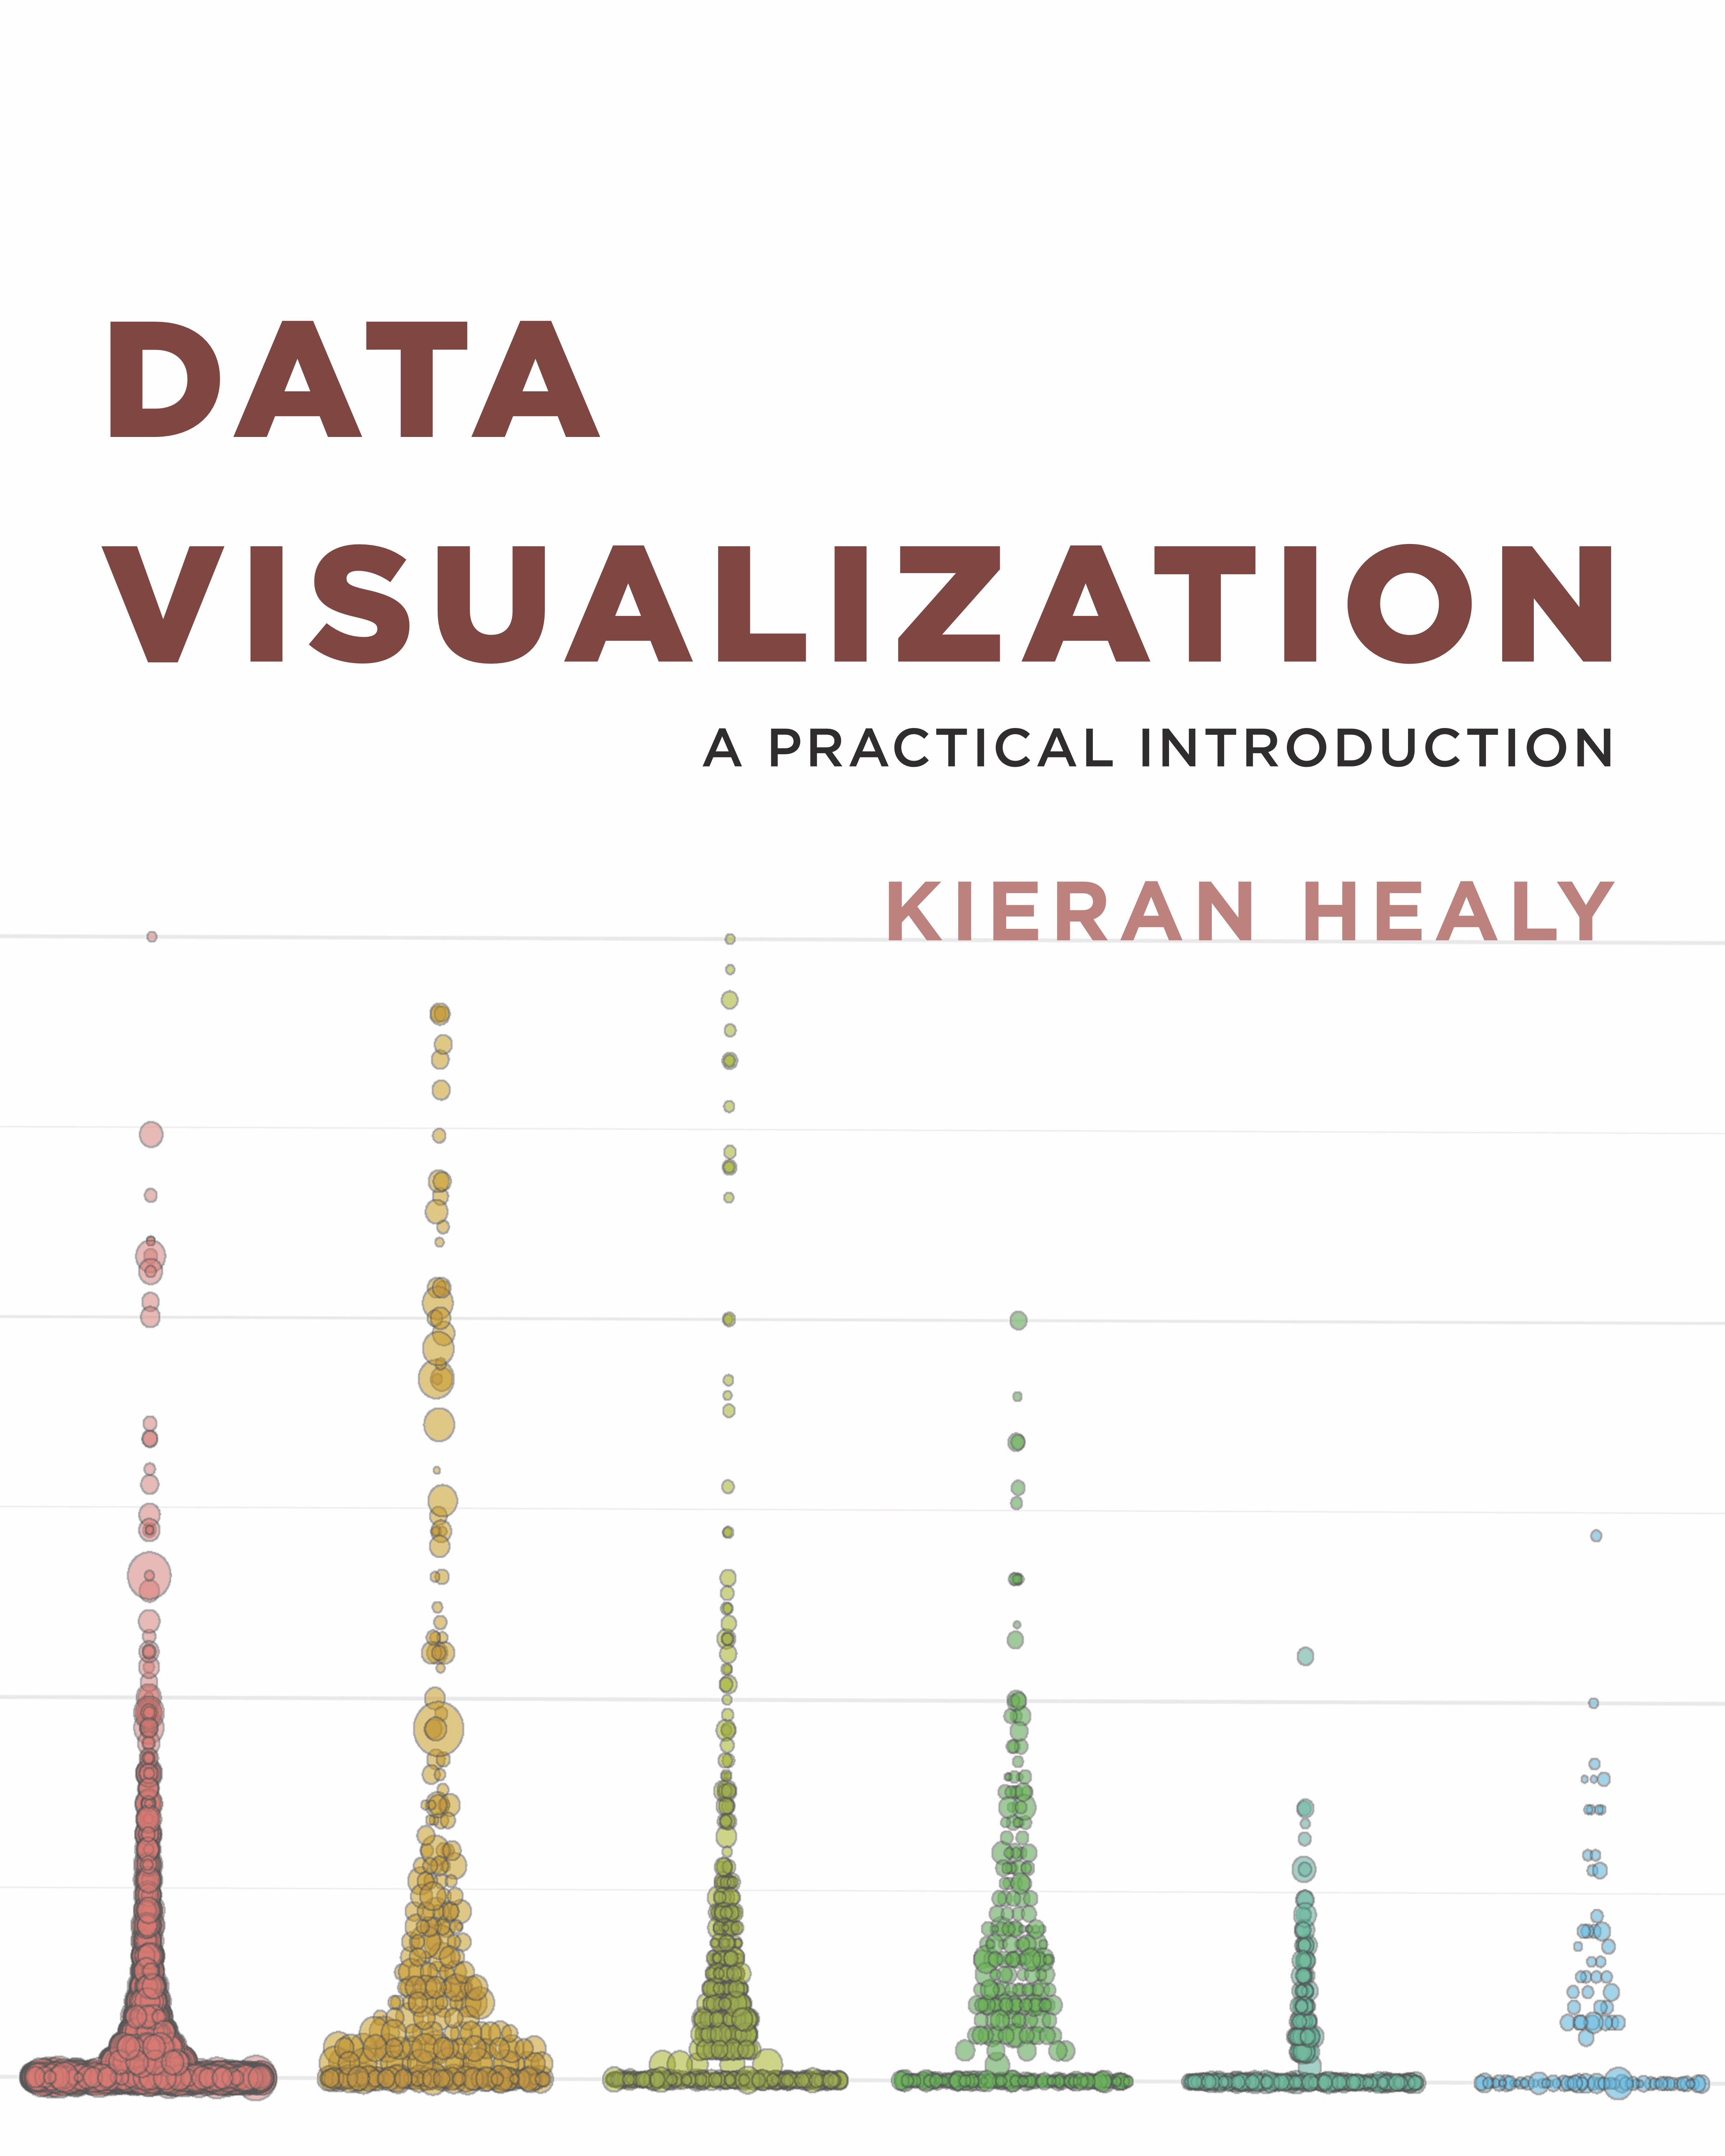
\includegraphics[width=0.3\textwidth,height=\textheight]{../images/healey.jpg}} \href{https://serialmentor.com/dataviz/}{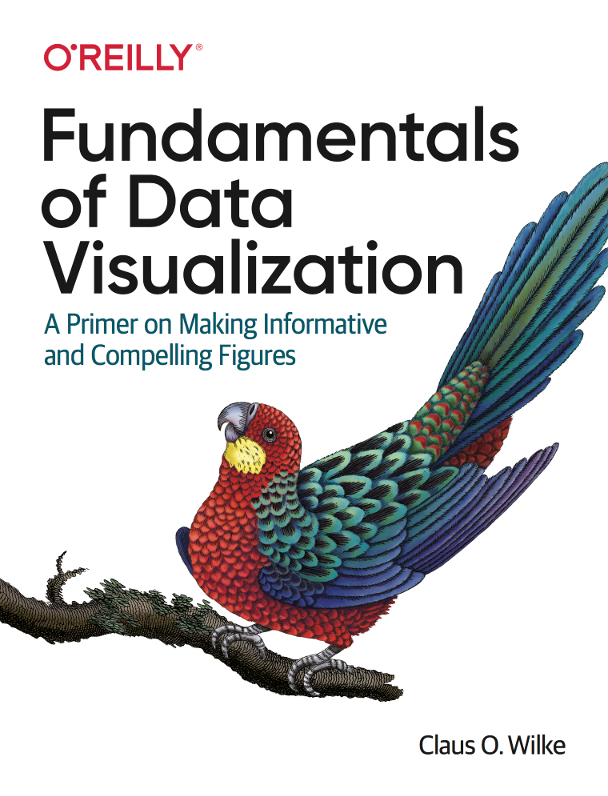
\includegraphics[width=0.3\textwidth,height=\textheight]{../images/wilke.png}}

~~

First I'd like you to watch this brief video where I give some examples of the kinds of data visualisations you can build in R, and why you probably want to avoid building bar graphs.

~~

~~

~~

\hypertarget{the-basics-of-ggplot2}{%
\section{The Basics of ggplot2}\label{the-basics-of-ggplot2}}

First we need to load the ggplot2 package. As it is part of the Tidyverse (and we're likely to be using other Tidyverse packages alongside ggplot2), we load it into our library using the \texttt{library(tidyverse)} line of code.

\begin{Shaded}
\begin{Highlighting}[]
\FunctionTok{library}\NormalTok{(tidyverse)}
\end{Highlighting}
\end{Shaded}

In the video, I mention that using ggplot2 requires us to specify some core information in order to build our visualisations. These include the raw data that you want to plot, geometries (or geoms) that are the geometric shapes that will represent the data, and the aesthetics of the geometric and objects, such as color, size, shape and position.

\hypertarget{your-first-visualisation}{%
\section{Your First Visualisation}\label{your-first-visualisation}}

Below is an example where we're using the \texttt{mpg} dataset (which is a dataset that contains information about cars) to build a visualisation that plots the points corresponding to city fuel economy (\texttt{cty}) on the y-axis and \texttt{manufacturer} on the x-axis.

\begin{Shaded}
\begin{Highlighting}[]
\NormalTok{mpg }\SpecialCharTok{\%\textgreater{}\%}
  \FunctionTok{ggplot}\NormalTok{(}\FunctionTok{aes}\NormalTok{(}\AttributeTok{x =}\NormalTok{ manufacturer, }\AttributeTok{y =}\NormalTok{ cty)) }\SpecialCharTok{+} 
  \FunctionTok{geom\_point}\NormalTok{() }
\end{Highlighting}
\end{Shaded}

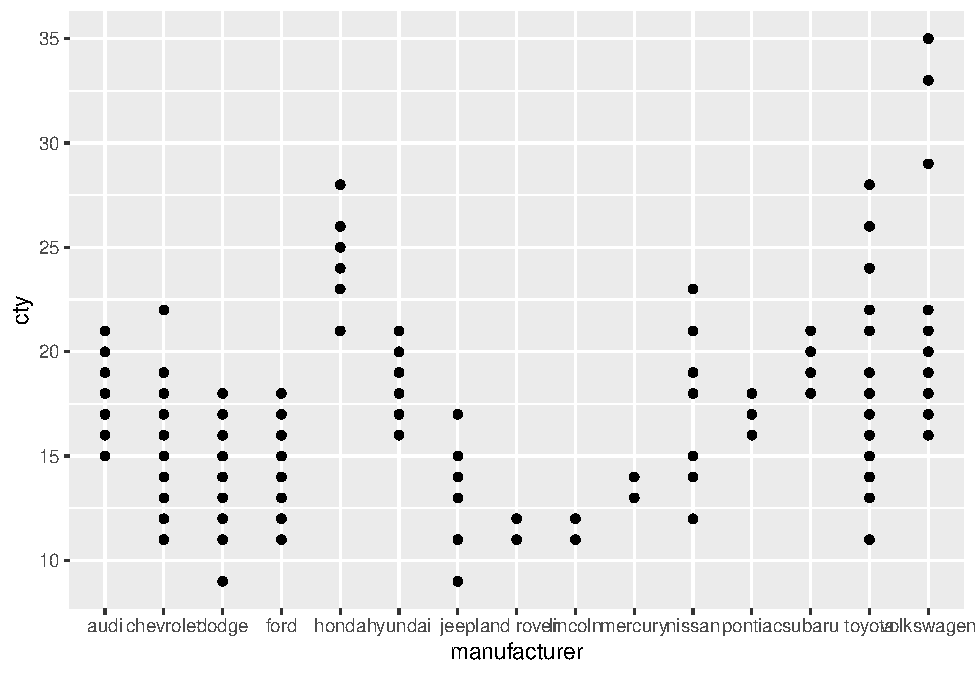
\includegraphics{_main_files/figure-latex/unnamed-chunk-49-1.pdf}

So, this is not great. The x-axis labels are hard to read, and the individual points don't look that pleasing. We can use the \texttt{str\_to\_title()} function to change the manufacturer labels to title case, and adjust the axis labels easily using the \texttt{theme()} function. Note, the \texttt{+} symbol between the lines of \texttt{ggplot()} code is equivalent to the \texttt{\%\textgreater{}\%} operator. For historical reasons (basically, because \texttt{ggplot()} came before the other packages in the Tidyverse), you need to use the \texttt{+} when adding layers to your \texttt{ggplot()} visualisations.

\begin{Shaded}
\begin{Highlighting}[]
\NormalTok{mpg }\SpecialCharTok{\%\textgreater{}\%}
  \FunctionTok{mutate}\NormalTok{(}\AttributeTok{manufacturer =} \FunctionTok{str\_to\_title}\NormalTok{(manufacturer)) }\SpecialCharTok{\%\textgreater{}\%}
  \FunctionTok{ggplot}\NormalTok{(}\FunctionTok{aes}\NormalTok{(}\AttributeTok{x =}\NormalTok{ manufacturer, }\AttributeTok{y =}\NormalTok{ cty)) }\SpecialCharTok{+} 
  \FunctionTok{geom\_point}\NormalTok{() }\SpecialCharTok{+}
  \FunctionTok{theme}\NormalTok{(}\AttributeTok{axis.text.x =} \FunctionTok{element\_text}\NormalTok{(}\AttributeTok{angle =} \DecValTok{45}\NormalTok{, }\AttributeTok{vjust =} \FloatTok{0.5}\NormalTok{, }\AttributeTok{hjust =}\NormalTok{ .}\DecValTok{5}\NormalTok{))}
\end{Highlighting}
\end{Shaded}

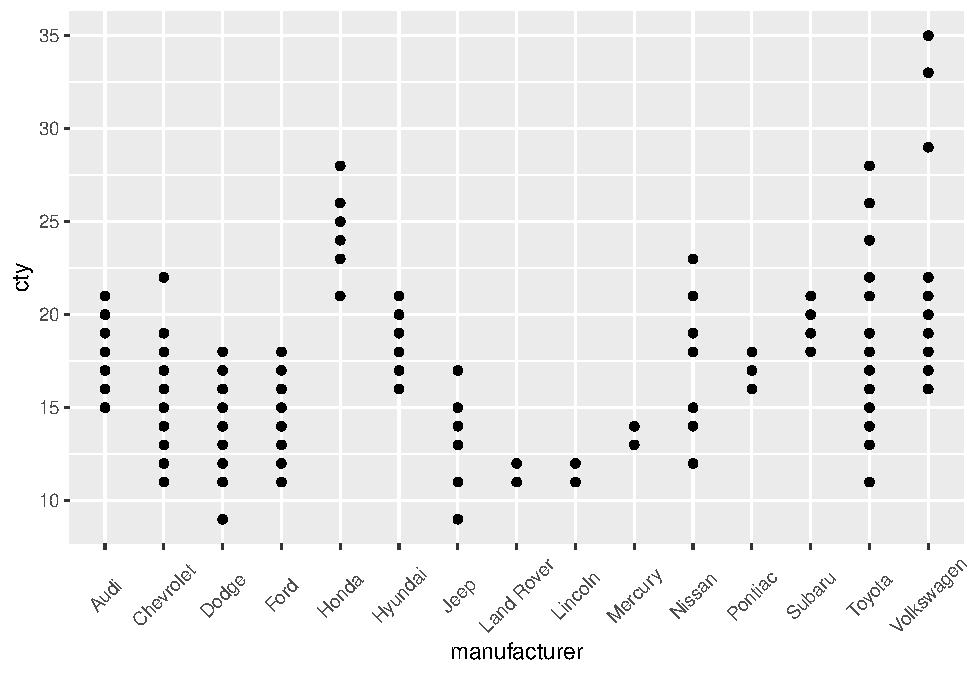
\includegraphics{_main_files/figure-latex/unnamed-chunk-50-1.pdf}

\hypertarget{improving-the-plot}{%
\subsection{Improving the Plot}\label{improving-the-plot}}

So let's do some more tidying - we're going to jitter the points slightly (so they're not stacked vertically) using the \texttt{geom\_jitter()} function, and tidy up the axis titles using the \texttt{labs()} function to explicitly add axis labels (rather than just use the labels in our dataset). We're also adding a few other tweaks - can you spot them?

\begin{Shaded}
\begin{Highlighting}[]
\NormalTok{mpg }\SpecialCharTok{\%\textgreater{}\%}
  \FunctionTok{mutate}\NormalTok{(}\AttributeTok{manufacturer =} \FunctionTok{str\_to\_title}\NormalTok{(manufacturer)) }\SpecialCharTok{\%\textgreater{}\%}
  \FunctionTok{ggplot}\NormalTok{(}\FunctionTok{aes}\NormalTok{(}\AttributeTok{x =}\NormalTok{ manufacturer, }\AttributeTok{y =}\NormalTok{ cty)) }\SpecialCharTok{+} 
  \FunctionTok{geom\_jitter}\NormalTok{(}\AttributeTok{width =}\NormalTok{ .}\DecValTok{2}\NormalTok{, }\AttributeTok{alpha =}\NormalTok{ .}\DecValTok{75}\NormalTok{, }\AttributeTok{size =} \DecValTok{2}\NormalTok{) }\SpecialCharTok{+} 
  \FunctionTok{theme\_minimal}\NormalTok{() }\SpecialCharTok{+}
  \FunctionTok{theme}\NormalTok{(}\AttributeTok{axis.text.x =} \FunctionTok{element\_text}\NormalTok{(}\AttributeTok{angle =} \DecValTok{45}\NormalTok{, }\AttributeTok{vjust =} \FloatTok{0.5}\NormalTok{, }\AttributeTok{hjust =}\NormalTok{ .}\DecValTok{5}\NormalTok{)) }\SpecialCharTok{+}
  \FunctionTok{theme}\NormalTok{(}\AttributeTok{text =} \FunctionTok{element\_text}\NormalTok{(}\AttributeTok{size =} \DecValTok{13}\NormalTok{)) }\SpecialCharTok{+}
  \FunctionTok{labs}\NormalTok{(}\AttributeTok{title =} \StringTok{"City Fuel Economy by Car Manufacturer"}\NormalTok{,}
       \AttributeTok{x =} \StringTok{"Manufacturer"}\NormalTok{, }
       \AttributeTok{y =} \StringTok{"City Fuel Economy (mpg)"}\NormalTok{)}
\end{Highlighting}
\end{Shaded}

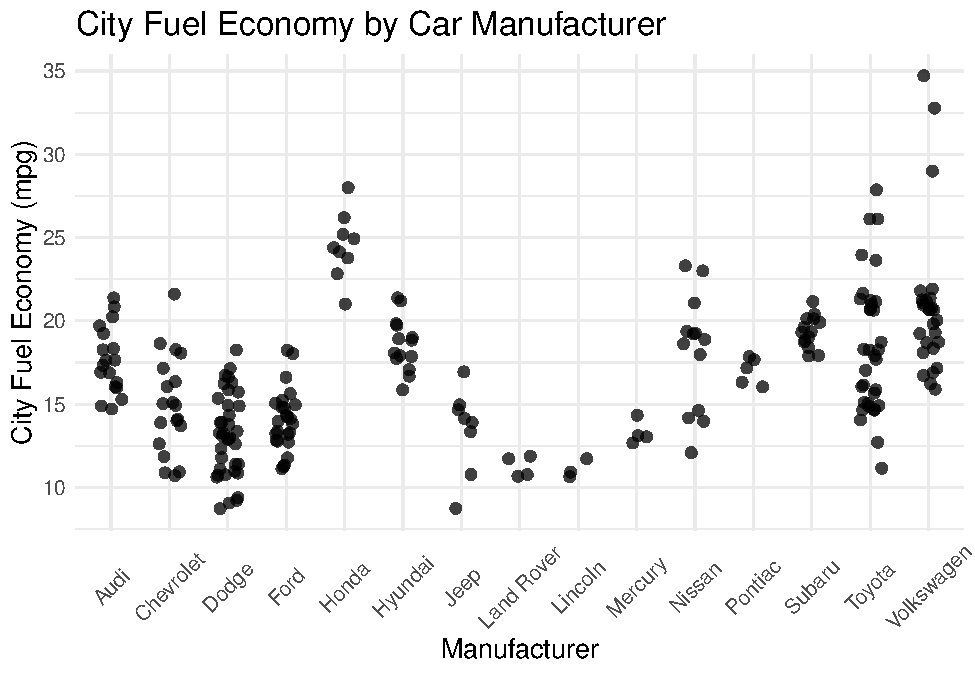
\includegraphics{_main_files/figure-latex/unnamed-chunk-51-1.pdf}

It might be helpful for us to add summary statistical information such as the mean fuel economy and confidence intervals around the mean for each car manufacturer.

\hypertarget{adding-summary-statistics}{%
\subsection{Adding Summary Statistics}\label{adding-summary-statistics}}

We need to add the \texttt{Hmisc} package to allow us to use the \texttt{stat\_summary()} function.

\begin{Shaded}
\begin{Highlighting}[]
\FunctionTok{library}\NormalTok{(Hmisc)}
\end{Highlighting}
\end{Shaded}

\begin{Shaded}
\begin{Highlighting}[]
\NormalTok{mpg }\SpecialCharTok{\%\textgreater{}\%}
  \FunctionTok{mutate}\NormalTok{(}\AttributeTok{manufacturer =} \FunctionTok{str\_to\_title}\NormalTok{(manufacturer)) }\SpecialCharTok{\%\textgreater{}\%}
  \FunctionTok{ggplot}\NormalTok{(}\FunctionTok{aes}\NormalTok{(}\AttributeTok{x =}\NormalTok{ manufacturer, }\AttributeTok{y =}\NormalTok{ cty)) }\SpecialCharTok{+} 
  \FunctionTok{stat\_summary}\NormalTok{(}\AttributeTok{fun.data =}\NormalTok{ mean\_cl\_boot, }\AttributeTok{colour =} \StringTok{"black"}\NormalTok{, }\AttributeTok{size =} \DecValTok{1}\NormalTok{) }\SpecialCharTok{+}
  \FunctionTok{theme\_minimal}\NormalTok{() }\SpecialCharTok{+}
  \FunctionTok{theme}\NormalTok{(}\AttributeTok{axis.text.x =} \FunctionTok{element\_text}\NormalTok{(}\AttributeTok{angle =} \DecValTok{45}\NormalTok{, }\AttributeTok{vjust =} \FloatTok{0.5}\NormalTok{, }\AttributeTok{hjust =}\NormalTok{ .}\DecValTok{5}\NormalTok{)) }\SpecialCharTok{+}
  \FunctionTok{theme}\NormalTok{(}\AttributeTok{text =} \FunctionTok{element\_text}\NormalTok{(}\AttributeTok{size =} \DecValTok{13}\NormalTok{)) }\SpecialCharTok{+}
  \FunctionTok{labs}\NormalTok{(}\AttributeTok{title =} \StringTok{"City Fuel Economy by Car Manufacturer"}\NormalTok{,}
       \AttributeTok{x =} \StringTok{"Manufacturer"}\NormalTok{, }
       \AttributeTok{y =} \StringTok{"City Fuel Economy (mpg)"}\NormalTok{)}
\end{Highlighting}
\end{Shaded}

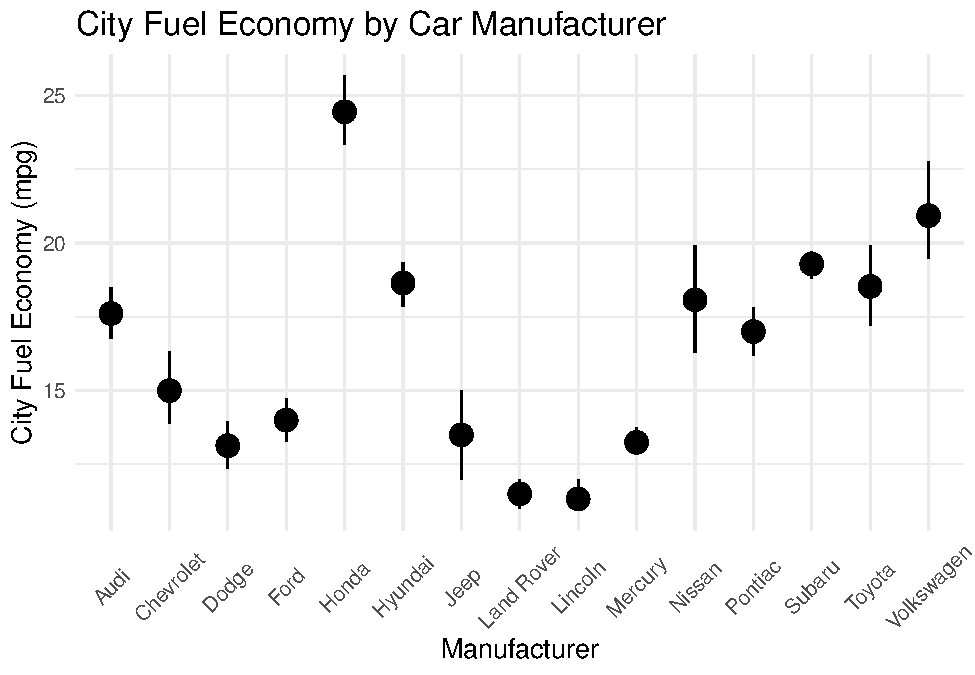
\includegraphics{_main_files/figure-latex/unnamed-chunk-53-1.pdf}

\hypertarget{the-finished-plot}{%
\subsection{The Finished(?) Plot}\label{the-finished-plot}}

At the moment, the x-axis is ordered alphabetically. How about we order it so that it goes from manufacturer with the hightest mean fuel economy, to the lowest. Also, how about we flip the visualisation so that the axes swap and add a few other tweaks?

\begin{Shaded}
\begin{Highlighting}[]
\NormalTok{mpg }\SpecialCharTok{\%\textgreater{}\%}
  \FunctionTok{mutate}\NormalTok{(}\AttributeTok{manufacturer =} \FunctionTok{str\_to\_title}\NormalTok{(manufacturer)) }\SpecialCharTok{\%\textgreater{}\%}
  \FunctionTok{ggplot}\NormalTok{(}\FunctionTok{aes}\NormalTok{(}\AttributeTok{x =} \FunctionTok{fct\_reorder}\NormalTok{(manufacturer, }\AttributeTok{.fun =}\NormalTok{ mean, cty), }\AttributeTok{y =}\NormalTok{ cty, }\AttributeTok{colour =}\NormalTok{ manufacturer)) }\SpecialCharTok{+}
  \FunctionTok{stat\_summary}\NormalTok{(}\AttributeTok{fun.data =}\NormalTok{ mean\_cl\_boot, }\AttributeTok{size =} \DecValTok{1}\NormalTok{) }\SpecialCharTok{+}
  \FunctionTok{geom\_jitter}\NormalTok{(}\AttributeTok{alpha =}\NormalTok{ .}\DecValTok{25}\NormalTok{) }\SpecialCharTok{+}
  \FunctionTok{theme\_minimal}\NormalTok{() }\SpecialCharTok{+}
  \FunctionTok{theme}\NormalTok{(}\AttributeTok{text =} \FunctionTok{element\_text}\NormalTok{(}\AttributeTok{size =} \DecValTok{13}\NormalTok{)) }\SpecialCharTok{+}
  \FunctionTok{labs}\NormalTok{(}\AttributeTok{title =} \StringTok{"Manufacturer by City Fuel Economy"}\NormalTok{,}
       \AttributeTok{x =} \StringTok{"Manufacturer"}\NormalTok{, }
       \AttributeTok{y =} \StringTok{"City Fuel Economy (mpg)"}\NormalTok{) }\SpecialCharTok{+}
  \FunctionTok{guides}\NormalTok{(}\AttributeTok{colour =} \StringTok{\textquotesingle{}none\textquotesingle{}}\NormalTok{) }\SpecialCharTok{+}
  \FunctionTok{coord\_flip}\NormalTok{()}
\end{Highlighting}
\end{Shaded}

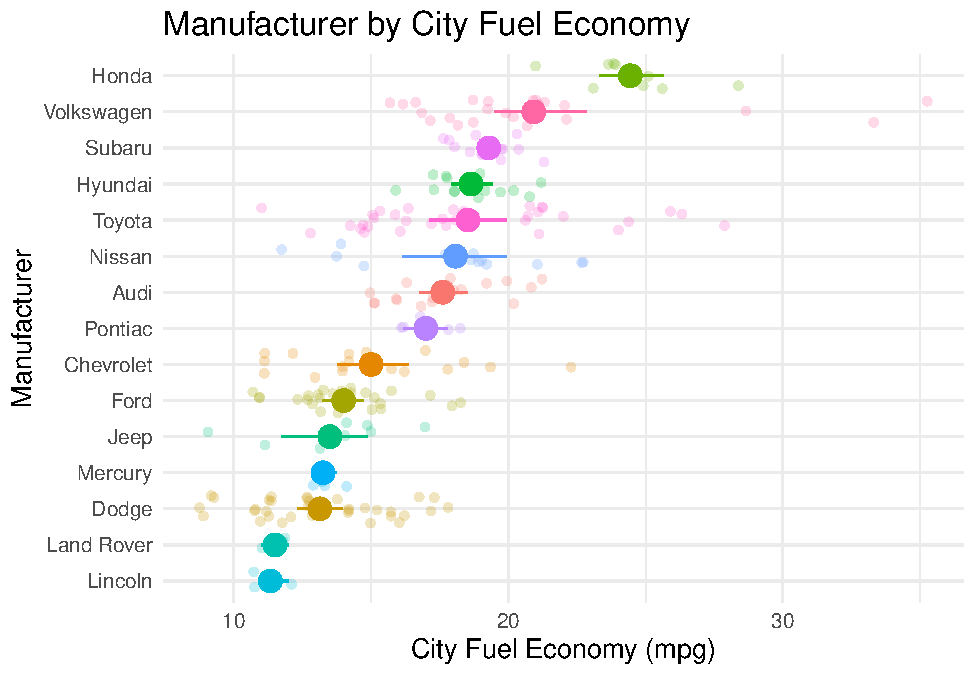
\includegraphics{_main_files/figure-latex/unnamed-chunk-54-1.pdf}

This is looks pretty good. Can you tell what the other bits of code do that I added? Have a go changing some of the numbers to see what happens. You can prevent a line of code being run by adding a \texttt{\#} in front of it. So if you need to temporarily not run a line, just add a \texttt{\#} rather than delete the line.

Plots are rarely completely ``finished'' as you'll often think of a minor aesthetic tweak that might make some improvement.

\hypertarget{using-facet_wrap}{%
\subsection{\texorpdfstring{Using \texttt{facet\_wrap()}}{Using facet\_wrap()}}\label{using-facet_wrap}}

We might think that fuel economy varies as a function of the type of vehicle (e.g., sports cars may be more fuel hungry than midsize cars) and by the number size of engine (e.g., cars with bigger engines may be more fuel hungry). In the visualisation below we're going to use the \texttt{facet\_wrap()} function to build a separate visualisation for each level of the factor we are facetting over (ignoring SUVs).

\begin{Shaded}
\begin{Highlighting}[]
\NormalTok{mpg }\SpecialCharTok{\%\textgreater{}\%}
  \FunctionTok{filter}\NormalTok{(class }\SpecialCharTok{!=} \StringTok{"suv"}\NormalTok{) }\SpecialCharTok{\%\textgreater{}\%}
  \FunctionTok{mutate}\NormalTok{(}\AttributeTok{class =} \FunctionTok{str\_to\_title}\NormalTok{(class)) }\SpecialCharTok{\%\textgreater{}\%}
  \FunctionTok{ggplot}\NormalTok{(}\FunctionTok{aes}\NormalTok{(}\AttributeTok{x =}\NormalTok{ displ, }\AttributeTok{y =}\NormalTok{ cty, }\AttributeTok{colour =}\NormalTok{ class)) }\SpecialCharTok{+} 
  \FunctionTok{geom\_jitter}\NormalTok{(}\AttributeTok{width =}\NormalTok{ .}\DecValTok{2}\NormalTok{) }\SpecialCharTok{+}
  \FunctionTok{theme\_minimal}\NormalTok{() }\SpecialCharTok{+}
  \FunctionTok{theme}\NormalTok{(}\AttributeTok{text =} \FunctionTok{element\_text}\NormalTok{(}\AttributeTok{size =} \DecValTok{13}\NormalTok{)) }\SpecialCharTok{+}
  \FunctionTok{labs}\NormalTok{(}\AttributeTok{title =} \StringTok{"City Fuel Economy by Engine Displacement"}\NormalTok{,}
       \AttributeTok{x =} \StringTok{"Engine Displacement (litres)"}\NormalTok{, }
       \AttributeTok{y =} \StringTok{"City Fuel Economy (mpg)"}\NormalTok{) }\SpecialCharTok{+}
  \FunctionTok{guides}\NormalTok{(}\AttributeTok{colour =} \StringTok{\textquotesingle{}none\textquotesingle{}}\NormalTok{) }\SpecialCharTok{+}
  \FunctionTok{facet\_wrap}\NormalTok{(}\SpecialCharTok{\textasciitilde{}}\NormalTok{ class)}
\end{Highlighting}
\end{Shaded}

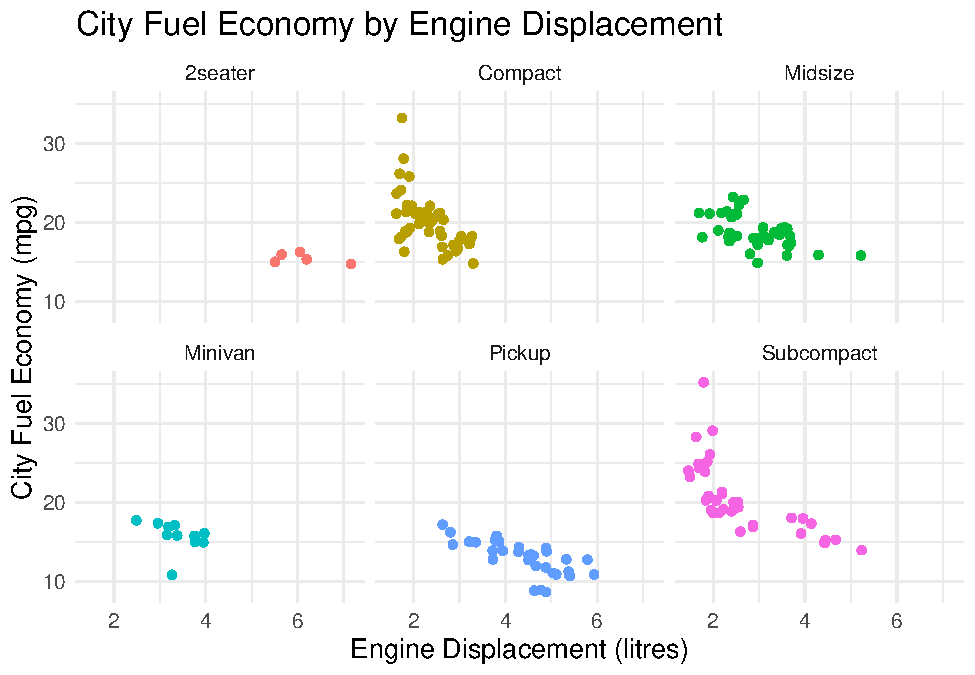
\includegraphics{_main_files/figure-latex/unnamed-chunk-55-1.pdf}

Can you tell what each of code is doing? Again, edit the numbers and put a \texttt{\#} before lines you want to temporarily ignore to see what happens.

\hypertarget{scatterplots}{%
\section{Scatterplots}\label{scatterplots}}

Above we focused on plotting a numerical variable on one axis, and a categorical variable on the other. There will be cases where we want to create scatterplots, allowing us to plot two numerical variables against each other - possibly to determine whether there might be a relationship between the two. Below we are plotting Engine Displacement on the y-axis, and City Fuel Economy on the x-axis.

\begin{Shaded}
\begin{Highlighting}[]
\NormalTok{mpg }\SpecialCharTok{\%\textgreater{}\%}
  \FunctionTok{mutate}\NormalTok{(}\AttributeTok{class =} \FunctionTok{str\_to\_upper}\NormalTok{(class)) }\SpecialCharTok{\%\textgreater{}\%}
  \FunctionTok{ggplot}\NormalTok{(}\FunctionTok{aes}\NormalTok{(}\AttributeTok{x =}\NormalTok{ cty, }\AttributeTok{y =}\NormalTok{ displ)) }\SpecialCharTok{+}
  \FunctionTok{geom\_point}\NormalTok{(}\FunctionTok{aes}\NormalTok{(}\AttributeTok{colour =}\NormalTok{ class)) }\SpecialCharTok{+}
  \FunctionTok{geom\_smooth}\NormalTok{(}\AttributeTok{se =} \ConstantTok{FALSE}\NormalTok{) }\SpecialCharTok{+}
  \FunctionTok{theme}\NormalTok{(}\AttributeTok{text =} \FunctionTok{element\_text}\NormalTok{(}\AttributeTok{size =} \DecValTok{13}\NormalTok{)) }\SpecialCharTok{+}
  \FunctionTok{theme\_minimal}\NormalTok{() }\SpecialCharTok{+} 
  \FunctionTok{labs}\NormalTok{(}\AttributeTok{x =} \StringTok{"City Fuel Economy (mpg)"}\NormalTok{,}
       \AttributeTok{y =} \StringTok{"Engine Displacement (litres)"}\NormalTok{, }
       \AttributeTok{colour =} \StringTok{"Vehicle Class"}\NormalTok{)}
\end{Highlighting}
\end{Shaded}

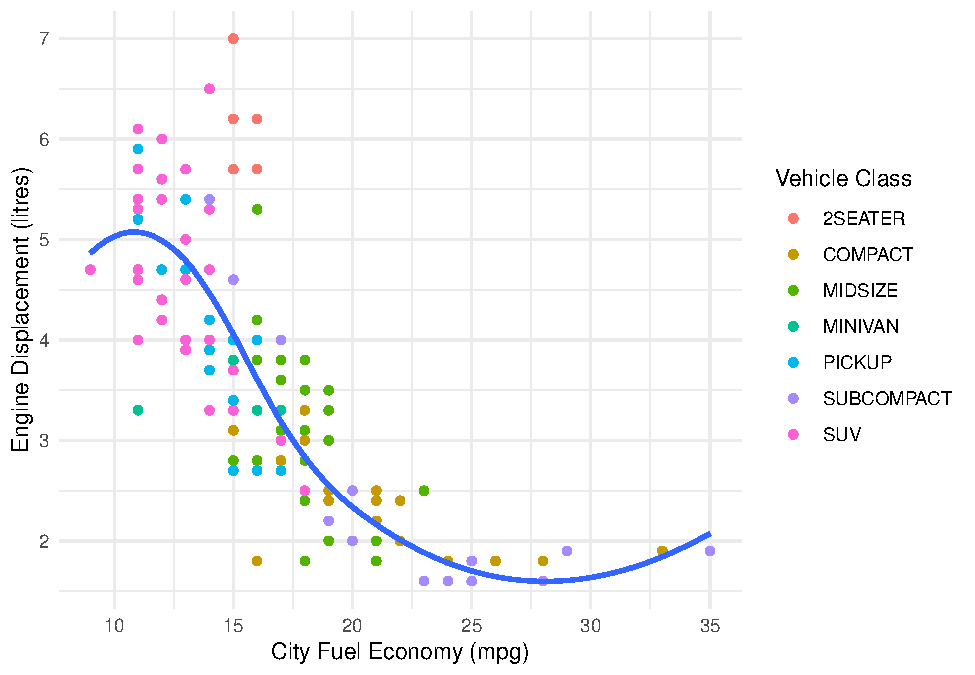
\includegraphics{_main_files/figure-latex/unnamed-chunk-56-1.pdf}

In the above example, we used the \texttt{geom\_smooth()} function to add a layer corresponding to fitting a curve to our data. We can see a fairly clear negative correlation between Engine Displacement and Fuel Economhy for Fuel Economy values that are less than 25 mpg, but little relationship between the two for values that are great than 25 mpg. These seems to suggest there are some cars with relaitively small engines that have great fuel economy, and others with similar engine sizes were much worse fuel economy.

\hypertarget{plotting-histograms}{%
\section{Plotting Histograms}\label{plotting-histograms}}

We might want to plot a histogram of engine sizes (measured in litres and captured in the variable \texttt{displ} in the \texttt{mpg} dataset) to get a feel for how this variable is distributed.

\begin{Shaded}
\begin{Highlighting}[]
\NormalTok{mpg }\SpecialCharTok{\%\textgreater{}\%}
  \FunctionTok{ggplot}\NormalTok{(}\FunctionTok{aes}\NormalTok{(}\AttributeTok{x =}\NormalTok{ displ)) }\SpecialCharTok{+}
  \FunctionTok{geom\_histogram}\NormalTok{(}\AttributeTok{binwidth =}\NormalTok{ .}\DecValTok{5}\NormalTok{, }\AttributeTok{fill =} \StringTok{"grey"}\NormalTok{) }\SpecialCharTok{+}
  \FunctionTok{labs}\NormalTok{(}\AttributeTok{title =} \StringTok{"Histogram of Engine Displacement"}\NormalTok{,}
       \AttributeTok{x =} \StringTok{"Engine Displacement (litres)"}\NormalTok{,}
       \AttributeTok{y =} \StringTok{"Count"}\NormalTok{)}
\end{Highlighting}
\end{Shaded}

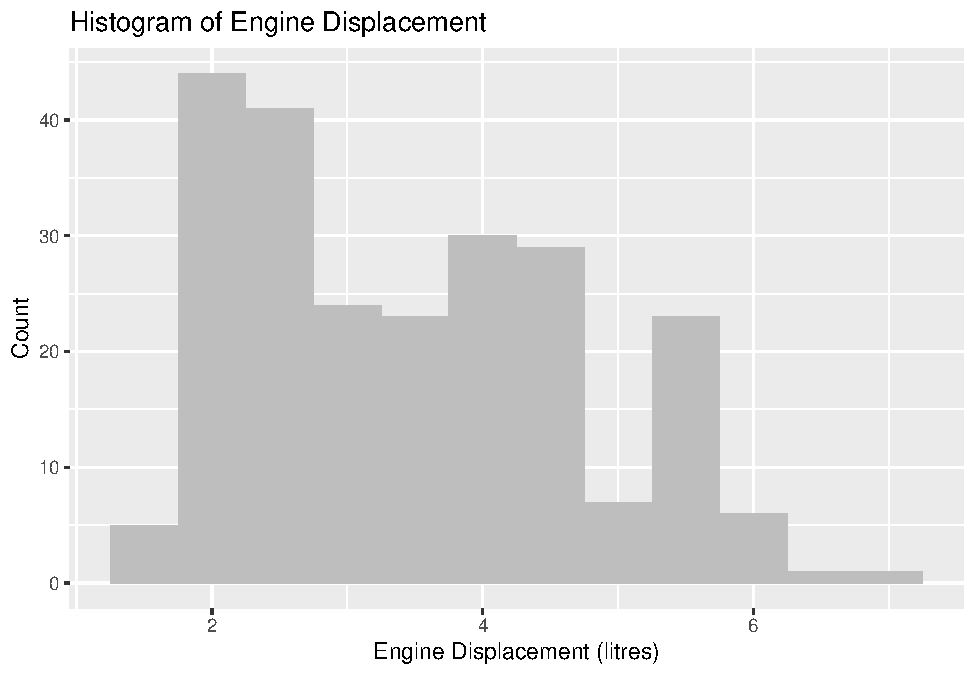
\includegraphics{_main_files/figure-latex/unnamed-chunk-57-1.pdf}

\hypertarget{the-ggridges-package}{%
\subsection{\texorpdfstring{The \texttt{ggridges} Package}{The ggridges Package}}\label{the-ggridges-package}}

Given in a previous visualisation we saw that there seemed to be variability between vehicle classes, wouldn't it be great if we could compare the distributions of engine size separated by vehicle class? We're now going to use the \texttt{ggridges()} package to do just that\ldots{}

\begin{Shaded}
\begin{Highlighting}[]
\FunctionTok{library}\NormalTok{(ggridges)}
\end{Highlighting}
\end{Shaded}

\begin{Shaded}
\begin{Highlighting}[]
\NormalTok{mpg }\SpecialCharTok{\%\textgreater{}\%}
  \FunctionTok{mutate}\NormalTok{(}\AttributeTok{class =} \FunctionTok{str\_to\_title}\NormalTok{(class)) }\SpecialCharTok{\%\textgreater{}\%}
  \FunctionTok{ggplot}\NormalTok{(}\FunctionTok{aes}\NormalTok{(}\AttributeTok{x =}\NormalTok{ displ, }\AttributeTok{y =} \FunctionTok{fct\_reorder}\NormalTok{(class, }\AttributeTok{.fun =}\NormalTok{ mean, displ))) }\SpecialCharTok{+}
  \FunctionTok{geom\_density\_ridges}\NormalTok{(}\AttributeTok{height =}\NormalTok{ .}\DecValTok{5}\NormalTok{, }\FunctionTok{aes}\NormalTok{(}\AttributeTok{fill =}\NormalTok{ class)) }\SpecialCharTok{+}
  \FunctionTok{theme\_minimal}\NormalTok{() }\SpecialCharTok{+}
  \FunctionTok{theme}\NormalTok{(}\AttributeTok{text =} \FunctionTok{element\_text}\NormalTok{(}\AttributeTok{size =} \DecValTok{13}\NormalTok{)) }\SpecialCharTok{+}
  \FunctionTok{guides}\NormalTok{(}\AttributeTok{fill =} \StringTok{\textquotesingle{}none\textquotesingle{}}\NormalTok{) }\SpecialCharTok{+} 
  \FunctionTok{labs}\NormalTok{(}\AttributeTok{x =} \StringTok{"Engine Displacement (litres)"}\NormalTok{,}
       \AttributeTok{y =} \ConstantTok{NULL}\NormalTok{)}
\end{Highlighting}
\end{Shaded}

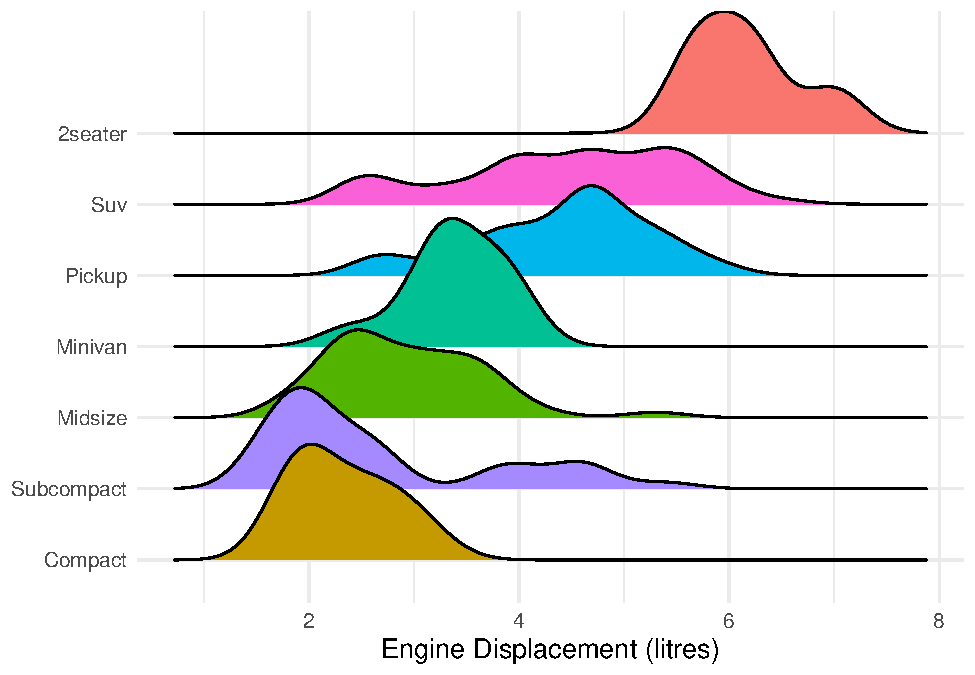
\includegraphics{_main_files/figure-latex/unnamed-chunk-59-1.pdf}

We can see from the above visualisation that SUVs seem to have quite a lot of variability in engine size while compact cars have relatively little variability.

\hypertarget{the-nhanes-dataset}{%
\section{The NHANES Dataset}\label{the-nhanes-dataset}}

We're now going to visualise aspects of the NHANES dataset.

~~

\begin{quote}
This is survey data collected by the US National Center for Health Statistics (NCHS) which has conducted a series of health and nutrition surveys since the early 1960's. Since 1999 approximately 5,000 individuals of all ages are interviewed in their homes every year and complete the health examination component of the survey. The health examination is conducted in a mobile examination centre (MEC). The NHANES target population is ``the non-institutionalized civilian resident population of the United States''. NHANES, (American National Health and Nutrition Examination surveys), use complex survey designs (see \url{http://www.cdc.gov/nchs/data/series/sr_02/sr02_162.pdf}) that oversample certain subpopulations like racial minorities. Naive analysis of the original NHANES data can lead to mistaken conclusions. The percentages of people from each racial group in the data, for example, are quite different from the way they are in the population.
\end{quote}

~~

We need to load the \texttt{NHANES} package as this is where the dataset is contained.

\begin{Shaded}
\begin{Highlighting}[]
\FunctionTok{library}\NormalTok{(NHANES)}
\end{Highlighting}
\end{Shaded}

If running the above command generated an error, is it because you haven't installed the packed on your machine with \texttt{install.packages("NHANES")}?

First we're going to explore the NHANES dataset.

\begin{Shaded}
\begin{Highlighting}[]
\FunctionTok{ncol}\NormalTok{(NHANES)}
\end{Highlighting}
\end{Shaded}

\begin{verbatim}
## [1] 76
\end{verbatim}

\begin{Shaded}
\begin{Highlighting}[]
\FunctionTok{nrow}\NormalTok{(NHANES)}
\end{Highlighting}
\end{Shaded}

\begin{verbatim}
## [1] 10000
\end{verbatim}

We see there are 76 columns and 10,000 rows. If we use the function \texttt{head()} we can see the first few rows of the dataframe.

\begin{Shaded}
\begin{Highlighting}[]
\FunctionTok{head}\NormalTok{(NHANES)}
\end{Highlighting}
\end{Shaded}

\begin{verbatim}
## # A tibble: 6 x 76
##      ID SurveyYr Gender   Age AgeDecade AgeMonths Race1 Race3 Education   
##   <int> <fct>    <fct>  <int> <fct>         <int> <fct> <fct> <fct>       
## 1 51624 2009_10  male      34 " 30-39"        409 White <NA>  High School 
## 2 51624 2009_10  male      34 " 30-39"        409 White <NA>  High School 
## 3 51624 2009_10  male      34 " 30-39"        409 White <NA>  High School 
## 4 51625 2009_10  male       4 " 0-9"           49 Other <NA>  <NA>        
## 5 51630 2009_10  female    49 " 40-49"        596 White <NA>  Some College
## 6 51638 2009_10  male       9 " 0-9"          115 White <NA>  <NA>        
## # i 67 more variables: MaritalStatus <fct>, HHIncome <fct>, HHIncomeMid <int>,
## #   Poverty <dbl>, HomeRooms <int>, HomeOwn <fct>, Work <fct>, Weight <dbl>,
## #   Length <dbl>, HeadCirc <dbl>, Height <dbl>, BMI <dbl>,
## #   BMICatUnder20yrs <fct>, BMI_WHO <fct>, Pulse <int>, BPSysAve <int>,
## #   BPDiaAve <int>, BPSys1 <int>, BPDia1 <int>, BPSys2 <int>, BPDia2 <int>,
## #   BPSys3 <int>, BPDia3 <int>, Testosterone <dbl>, DirectChol <dbl>,
## #   TotChol <dbl>, UrineVol1 <int>, UrineFlow1 <dbl>, UrineVol2 <int>, ...
\end{verbatim}

\hypertarget{tidying-the-data}{%
\subsection{Tidying the Data}\label{tidying-the-data}}

It looks like some participants appear more than once in the dataset - this could be due to the oversampling mentioned in the description - the first few rows are all for participant ID 51624. We can use the \texttt{select()} function alongwith the \texttt{n\_distinct()} function to tell us the unique number of IDs in the dataset.

\begin{Shaded}
\begin{Highlighting}[]
\NormalTok{NHANES }\SpecialCharTok{\%\textgreater{}\%} 
  \FunctionTok{select}\NormalTok{(ID) }\SpecialCharTok{\%\textgreater{}\%} 
  \FunctionTok{n\_distinct}\NormalTok{()}
\end{Highlighting}
\end{Shaded}

\begin{verbatim}
## [1] 6779
\end{verbatim}

We see we have 6,779 unique individuals. Let's tidy our data to remove duplicate IDs. Note that below we're using the pipe operator \texttt{\%\textgreater{}\%} You can read it as `and then' so it means we're taking the NHANES dataset and then filtering it keep just rows with distinct ID numbers. The pipe operator really helps with the readability of your data wrangling code and is an integral part of the tidyverse philosophy - tidy data and tidy code.

\begin{Shaded}
\begin{Highlighting}[]
\NormalTok{NHANES\_tidied }\OtherTok{\textless{}{-}}\NormalTok{ NHANES }\SpecialCharTok{\%\textgreater{}\%} 
  \FunctionTok{distinct}\NormalTok{(ID, }\AttributeTok{.keep\_all =} \ConstantTok{TRUE}\NormalTok{)}
\end{Highlighting}
\end{Shaded}

\begin{Shaded}
\begin{Highlighting}[]
\FunctionTok{ncol}\NormalTok{(NHANES\_tidied)}
\end{Highlighting}
\end{Shaded}

\begin{verbatim}
## [1] 76
\end{verbatim}

\begin{Shaded}
\begin{Highlighting}[]
\FunctionTok{nrow}\NormalTok{(NHANES\_tidied)}
\end{Highlighting}
\end{Shaded}

\begin{verbatim}
## [1] 6779
\end{verbatim}

OK, so our tidied dataset is assigned to the variable NHANES\_tidied and has 6,779 rows (but still 76 columns) - as we'd expect given we have 6,779 unique individuals.

\hypertarget{plotting-a-histogram}{%
\subsection{Plotting a Histogram}\label{plotting-a-histogram}}

Let's start exploring the data. We have lots of potential variables and relationships to explore. I see we have one labelled \texttt{Education} which is coded as a factor. We also have information related to health such as BMI - first of all lets plot a histogram of BMI.

\begin{Shaded}
\begin{Highlighting}[]
\NormalTok{NHANES\_tidied }\SpecialCharTok{\%\textgreater{}\%}
  \FunctionTok{ggplot}\NormalTok{(}\FunctionTok{aes}\NormalTok{(}\AttributeTok{x =}\NormalTok{ BMI)) }\SpecialCharTok{+} 
  \FunctionTok{geom\_histogram}\NormalTok{(}\AttributeTok{bins =} \DecValTok{100}\NormalTok{, }\AttributeTok{na.rm =} \ConstantTok{TRUE}\NormalTok{)}
\end{Highlighting}
\end{Shaded}

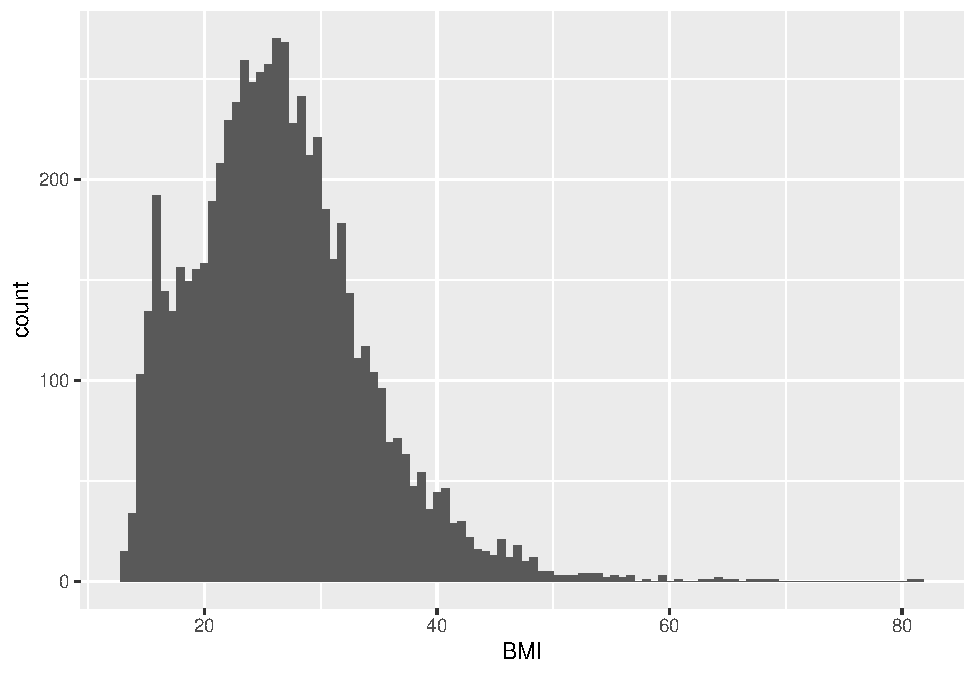
\includegraphics{_main_files/figure-latex/unnamed-chunk-66-1.pdf}

We see a pretty right skewed distribution here. Note our use of the \texttt{na.rm} parameter - this parameter appears in many tidyverse functions and by setting it to TRUE we tell R to ignore any parts of our data frame where we have missing data (which is indicated by \texttt{NA}).

\hypertarget{summary-statistics}{%
\subsection{Summary Statistics}\label{summary-statistics}}

Does BMI vary as a function of Education level? In the code below we are using the data stored in the variable \texttt{NHANES\_tidied}, grouping it by Education, then summarising to generate the median BMI for each of our groups. Again, we use the \texttt{na.rm\ =\ TRUE} parameter with the \texttt{summarise()} function this time to remove any missing values (\texttt{NA}) from our calculation.

\begin{Shaded}
\begin{Highlighting}[]
\NormalTok{NHANES\_tidied }\SpecialCharTok{\%\textgreater{}\%} 
  \FunctionTok{group\_by}\NormalTok{(Education) }\SpecialCharTok{\%\textgreater{}\%} 
  \FunctionTok{summarise}\NormalTok{(}\AttributeTok{median =} \FunctionTok{median}\NormalTok{(BMI, }\AttributeTok{na.rm =} \ConstantTok{TRUE}\NormalTok{))}
\end{Highlighting}
\end{Shaded}

\begin{verbatim}
## # A tibble: 6 x 2
##   Education      median
##   <fct>           <dbl>
## 1 8th Grade        28.6
## 2 9 - 11th Grade   28.2
## 3 High School      28.2
## 4 Some College     28.4
## 5 College Grad     26.5
## 6 <NA>             18.9
\end{verbatim}

So it looks like those with College eduction have the lowest median BMI (ignoring the \texttt{NA} category which corresponds to cases where we don't have Education level recorded).

\hypertarget{geom_violin}{%
\subsection{\texorpdfstring{\texttt{geom\_violin()}}{geom\_violin()}}\label{geom_violin}}

Let's graph it! Note here we're filtering out cases where we don't have BMI value recorded. The function \texttt{is.na()} returns TRUE when applied to a case of missing data (\texttt{NA}) - we use the \texttt{!} operator to negate this and combine several of these expressions together using the logical AND operator \texttt{\&}.

The line of code below starting with \texttt{filter()} means filter cases where Education is not missing AND BMI is not missing. This means that the \texttt{NHANES\_tidied} data that gets passed to the \texttt{ggplot()} call has no missing data for the key variables we're interested in.

I then add a \texttt{geom\_violin()} layer to capture the shape of the distribution for each level of Education and \texttt{geom\_boxplot()} layer to create a boxplot for each level of our Education factor.

The \texttt{guides(colour\ =\ \textquotesingle{}none\textquotesingle{})} call suppresses displaying the colour legend - place a \texttt{\#} in front of it and rerun the code to see what changes.

\begin{Shaded}
\begin{Highlighting}[]
\NormalTok{NHANES\_tidied }\SpecialCharTok{\%\textgreater{}\%} 
  \FunctionTok{filter}\NormalTok{(}\SpecialCharTok{!}\FunctionTok{is.na}\NormalTok{(Education) }\SpecialCharTok{\&} \SpecialCharTok{!}\FunctionTok{is.na}\NormalTok{(BMI)) }\SpecialCharTok{\%\textgreater{}\%}
  \FunctionTok{ggplot}\NormalTok{(}\FunctionTok{aes}\NormalTok{(}\AttributeTok{x =}\NormalTok{ Education, }\AttributeTok{y =}\NormalTok{ BMI, }\AttributeTok{colour =}\NormalTok{ Education)) }\SpecialCharTok{+} 
  \FunctionTok{geom\_violin}\NormalTok{() }\SpecialCharTok{+}
  \FunctionTok{geom\_jitter}\NormalTok{(}\AttributeTok{alpha =}\NormalTok{ .}\DecValTok{2}\NormalTok{, }\AttributeTok{width =}\NormalTok{ .}\DecValTok{1}\NormalTok{) }\SpecialCharTok{+}
  \FunctionTok{geom\_boxplot}\NormalTok{(}\AttributeTok{alpha =}\NormalTok{ .}\DecValTok{5}\NormalTok{) }\SpecialCharTok{+}
  \FunctionTok{guides}\NormalTok{(}\AttributeTok{colour =} \StringTok{\textquotesingle{}none\textquotesingle{}}\NormalTok{) }\SpecialCharTok{+} 
  \FunctionTok{labs}\NormalTok{(}\AttributeTok{title =} \StringTok{"Examining the effect of education level on BMI"}\NormalTok{, }
       \AttributeTok{x =} \StringTok{"Education Level"}\NormalTok{, }
       \AttributeTok{y =} \StringTok{"BMI"}\NormalTok{)}
\end{Highlighting}
\end{Shaded}

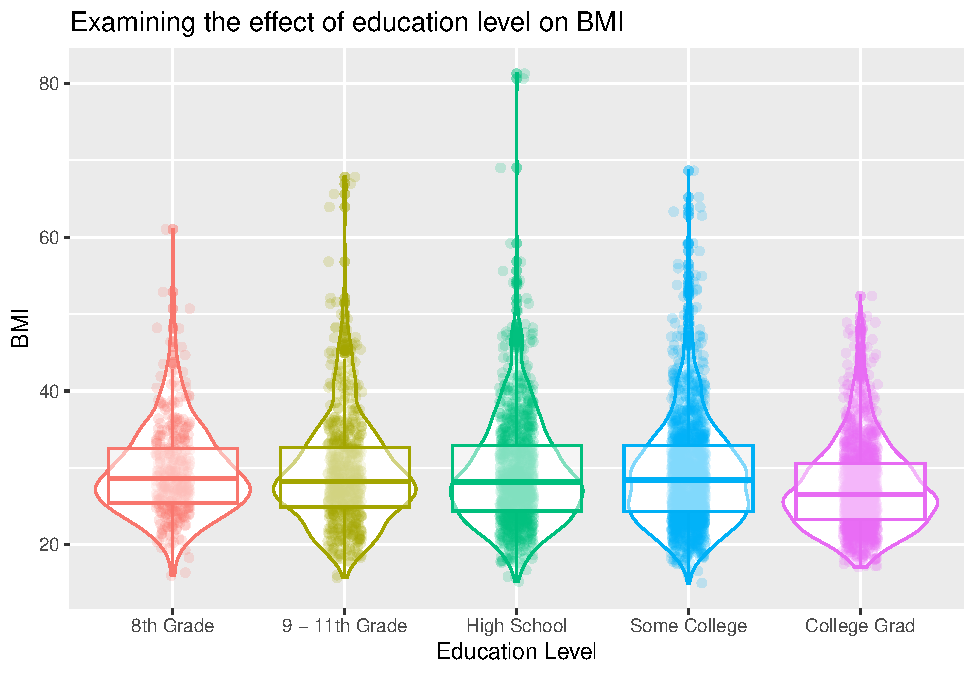
\includegraphics{_main_files/figure-latex/unnamed-chunk-68-1.pdf}

\hypertarget{plotting-interaction-effects}{%
\subsection{Plotting Interaction Effects}\label{plotting-interaction-effects}}

We can also plot how two factors interact with each other. For the plot above, we'll now add the factor \texttt{Diabetes} (which has two levels - Yes vs.~No) to see how that might interact with Education level. To capture the nature of this interaction, we use the expression \texttt{Education:Diabetes} when we specify the x-axis aesthetic. Note, I have rotated the x-axis labels 45 degrees to make them easier to read.

\begin{Shaded}
\begin{Highlighting}[]
\NormalTok{NHANES\_tidied }\SpecialCharTok{\%\textgreater{}\%} 
  \FunctionTok{filter}\NormalTok{(}\SpecialCharTok{!}\FunctionTok{is.na}\NormalTok{(Education) }\SpecialCharTok{\&} \SpecialCharTok{!}\FunctionTok{is.na}\NormalTok{(BMI) }\SpecialCharTok{\&} \SpecialCharTok{!}\FunctionTok{is.na}\NormalTok{(Diabetes)) }\SpecialCharTok{\%\textgreater{}\%}
  \FunctionTok{ggplot}\NormalTok{(}\FunctionTok{aes}\NormalTok{(}\AttributeTok{x =}\NormalTok{ Education}\SpecialCharTok{:}\NormalTok{Diabetes, }\AttributeTok{y =}\NormalTok{ BMI, }\AttributeTok{colour =}\NormalTok{ Education)) }\SpecialCharTok{+} 
  \FunctionTok{geom\_violin}\NormalTok{() }\SpecialCharTok{+}
  \FunctionTok{geom\_jitter}\NormalTok{(}\AttributeTok{alpha =}\NormalTok{ .}\DecValTok{2}\NormalTok{, }\AttributeTok{width =}\NormalTok{ .}\DecValTok{1}\NormalTok{) }\SpecialCharTok{+}
  \FunctionTok{geom\_boxplot}\NormalTok{(}\AttributeTok{alpha =}\NormalTok{ .}\DecValTok{5}\NormalTok{) }\SpecialCharTok{+}
  \FunctionTok{guides}\NormalTok{(}\AttributeTok{colour =} \StringTok{\textquotesingle{}none\textquotesingle{}}\NormalTok{) }\SpecialCharTok{+} 
  \FunctionTok{theme}\NormalTok{(}\AttributeTok{axis.text.x =} \FunctionTok{element\_text}\NormalTok{(}\AttributeTok{angle =} \DecValTok{45}\NormalTok{, }\AttributeTok{vjust =} \FloatTok{0.5}\NormalTok{)) }\SpecialCharTok{+}
  \FunctionTok{labs}\NormalTok{(}\AttributeTok{title =} \StringTok{"Examining the effect of education level and diabetes on BMI"}\NormalTok{, }
       \AttributeTok{x =} \StringTok{"Education Level x Diabetes"}\NormalTok{, }
       \AttributeTok{y =} \StringTok{"BMI"}\NormalTok{)}
\end{Highlighting}
\end{Shaded}

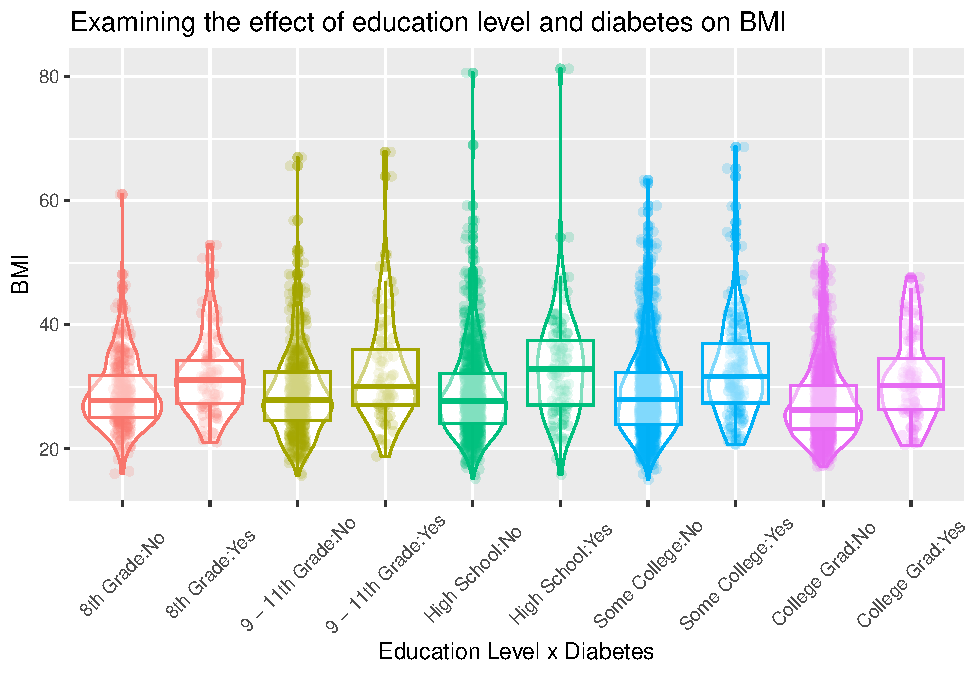
\includegraphics{_main_files/figure-latex/unnamed-chunk-69-1.pdf}

We can see from the above plot that those with Diabetes seem to also have higher BMI scores for each level of Education.

\hypertarget{histograms-with-facet_wrap}{%
\subsection{\texorpdfstring{Histograms with \texttt{facet\_wrap()}}{Histograms with facet\_wrap()}}\label{histograms-with-facet_wrap}}

We can also plot histograms of BMI separately for each Education level - we use the \texttt{facet\_wrap()} function to do this.

\begin{Shaded}
\begin{Highlighting}[]
\NormalTok{NHANES\_tidied }\SpecialCharTok{\%\textgreater{}\%} 
  \FunctionTok{filter}\NormalTok{(}\SpecialCharTok{!}\FunctionTok{is.na}\NormalTok{(Education) }\SpecialCharTok{\&} \SpecialCharTok{!}\FunctionTok{is.na}\NormalTok{(BMI)) }\SpecialCharTok{\%\textgreater{}\%}
  \FunctionTok{group\_by}\NormalTok{(Education) }\SpecialCharTok{\%\textgreater{}\%} 
  \FunctionTok{ggplot}\NormalTok{(}\FunctionTok{aes}\NormalTok{(}\AttributeTok{x =}\NormalTok{ BMI, }\AttributeTok{fill =}\NormalTok{ Education)) }\SpecialCharTok{+}
  \FunctionTok{geom\_histogram}\NormalTok{() }\SpecialCharTok{+}
  \FunctionTok{guides}\NormalTok{(}\AttributeTok{fill =} \StringTok{\textquotesingle{}none\textquotesingle{}}\NormalTok{) }\SpecialCharTok{+} 
  \FunctionTok{labs}\NormalTok{(}\AttributeTok{title =} \StringTok{"Examining the effect of education level on BMI"}\NormalTok{,}
       \AttributeTok{x =} \StringTok{"BMI"}\NormalTok{, }
       \AttributeTok{y =} \StringTok{"Number of cases"}\NormalTok{) }\SpecialCharTok{+} 
  \FunctionTok{facet\_wrap}\NormalTok{(}\SpecialCharTok{\textasciitilde{}}\NormalTok{ Education)}
\end{Highlighting}
\end{Shaded}

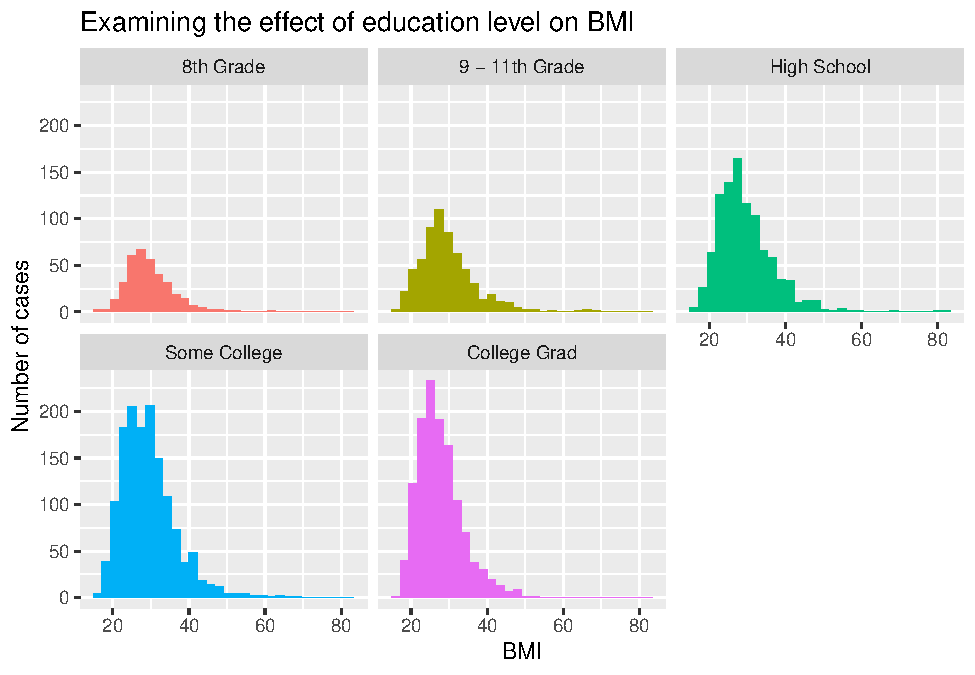
\includegraphics{_main_files/figure-latex/unnamed-chunk-70-1.pdf}

In the above graph, notice that the same y-axis scale is used for each plot - this makes comparisons a little tricky as there are different numbers of cases for each Eduction level. Add the following \texttt{scales\ =\ "free"} after \texttt{Education} in the \texttt{facet\_wrap()} line. What changes?

Instead of generating the histograms using a count, we could generate them using a density function. Let's also add a density curve.

\begin{Shaded}
\begin{Highlighting}[]
\NormalTok{NHANES\_tidied }\SpecialCharTok{\%\textgreater{}\%} 
  \FunctionTok{filter}\NormalTok{(}\SpecialCharTok{!}\FunctionTok{is.na}\NormalTok{(Education) }\SpecialCharTok{\&} \SpecialCharTok{!}\FunctionTok{is.na}\NormalTok{(BMI)) }\SpecialCharTok{\%\textgreater{}\%}
  \FunctionTok{group\_by}\NormalTok{(Education) }\SpecialCharTok{\%\textgreater{}\%} 
  \FunctionTok{ggplot}\NormalTok{(}\FunctionTok{aes}\NormalTok{(}\AttributeTok{x =}\NormalTok{ BMI, }\AttributeTok{fill =}\NormalTok{ Education)) }\SpecialCharTok{+}
  \FunctionTok{geom\_histogram}\NormalTok{(}\FunctionTok{aes}\NormalTok{(}\AttributeTok{y =}\NormalTok{ ..density..)) }\SpecialCharTok{+}
  \FunctionTok{geom\_density}\NormalTok{(}\FunctionTok{aes}\NormalTok{(}\AttributeTok{y =}\NormalTok{ ..density..)) }\SpecialCharTok{+}
  \FunctionTok{guides}\NormalTok{(}\AttributeTok{fill =} \StringTok{\textquotesingle{}none\textquotesingle{}}\NormalTok{) }\SpecialCharTok{+} 
  \FunctionTok{labs}\NormalTok{( }\AttributeTok{title =} \StringTok{"Examining the effect of education level on BMI"}\NormalTok{, }
        \AttributeTok{x =} \StringTok{"BMI"}\NormalTok{, }
        \AttributeTok{y =} \StringTok{"Density"}\NormalTok{) }\SpecialCharTok{+} 
  \FunctionTok{facet\_wrap}\NormalTok{(}\SpecialCharTok{\textasciitilde{}}\NormalTok{ Education)}
\end{Highlighting}
\end{Shaded}

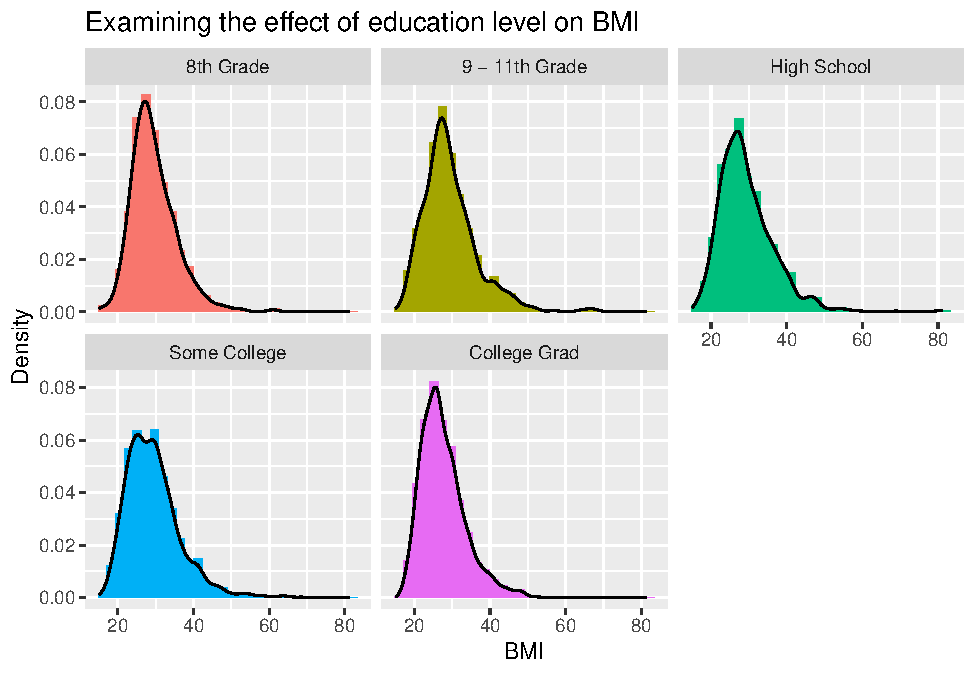
\includegraphics{_main_files/figure-latex/unnamed-chunk-71-1.pdf}

\hypertarget{your-challenge-do-this-in-the-live-session}{%
\section{Your Challenge (do this in the live session)}\label{your-challenge-do-this-in-the-live-session}}

Create some new visualisations with either the \texttt{mpg} or \texttt{NHANES} datasets. There are many possible visualisations you could build with either dataset.

\hypertarget{additional-resources}{%
\section{Additional Resources}\label{additional-resources}}

If you are interested in understanding more about ggplot2, you might be interested in watching these two (very) detailed webinars by Thomas Lin Pedersen, one of the developers working on ggplot2 and related packages.

\href{https://youtu.be/h29g21z0a68}{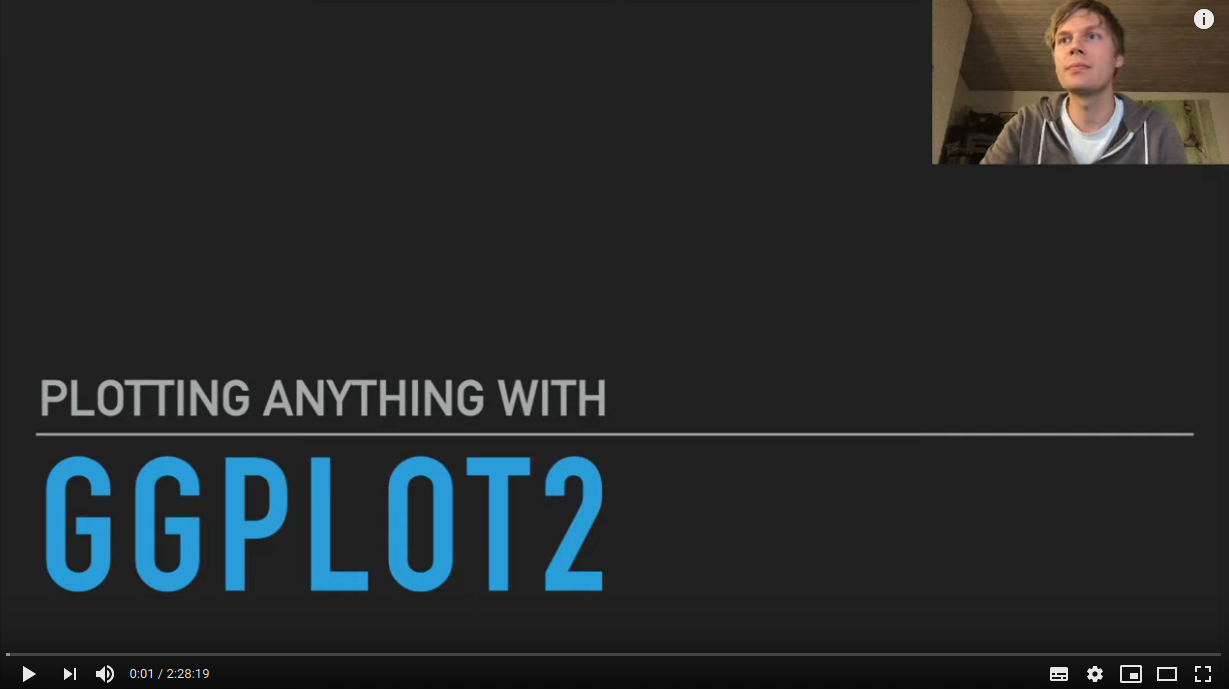
\includegraphics[width=0.75\textwidth,height=\textheight]{../images/ggplot2_pt1.png}}

\href{https://youtu.be/0m4yywqNPVY}{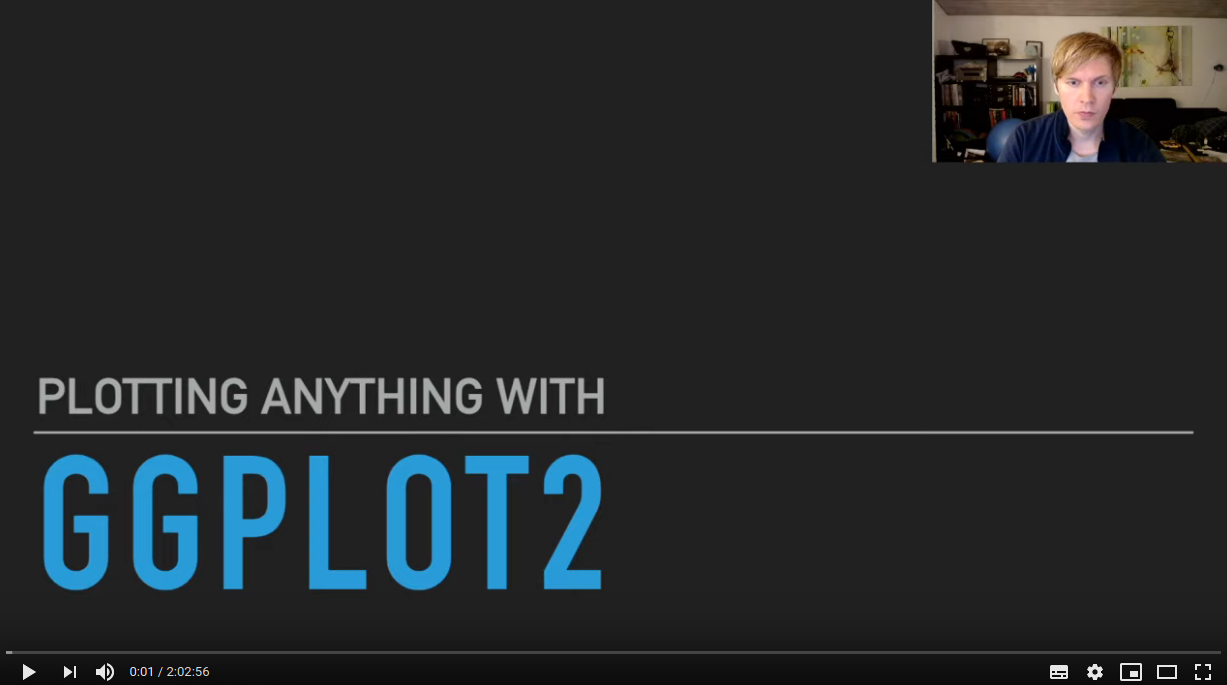
\includegraphics[width=0.75\textwidth,height=\textheight]{../images/ggplot2_pt2.png}}

\textbf{End of workshop 4 materials}

\hypertarget{r-markdown}{%
\chapter{R Markdown}\label{r-markdown}}

In this workshop we will see how to generate a report in .html format using R Markdown. Reports written using R Markdown allow you to combine narrative that you've written along with R code chunks, and the output associated with those code chunks all in one knitted document. The assignments for this unit need to be produced using R Markdown.

\hypertarget{overview}{%
\section{Overview}\label{overview}}

In the following video I will give you a brief overview of how you can turn a script you have written in R into an R Markdown document that you can `knit' and share with others.

~~

~~

There are many resources available to help you explore the full range of possibilities in R Markdown. A good starting point is the ``R Markdown: The Definitive Guide'' by Yihui Xie, J. J. Allaire, and Garrett Grolemund. Just click on the image below to be taken to the online version of the book.

~~

\href{https://bookdown.org/yihui/rmarkdown/}{
\includegraphics[width=0.5\textwidth,height=\textheight]{../images/r_markdown_guide.png}}

~~

You may also be interested in the ``R Markdown Cookbook'' by Yihui Xie, Christophe Dervieux, and Emily Riederer. Again, just click on the image below to be taken to the online version of the book.

~~

\href{https://bookdown.org/yihui/rmarkdown-cookbook/}{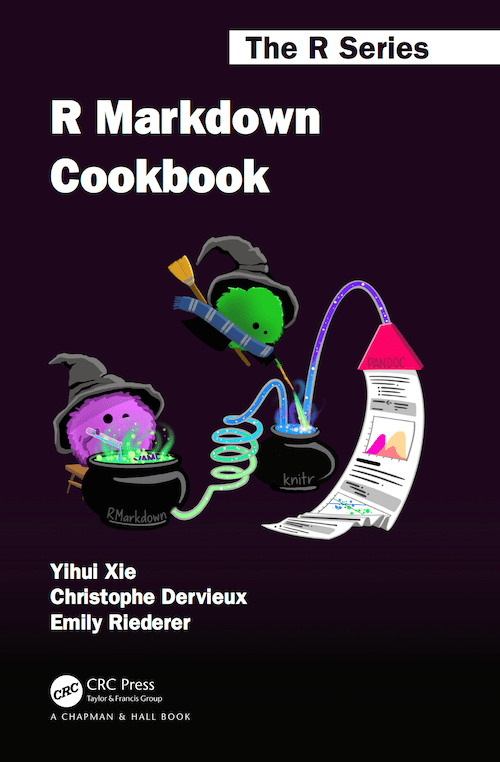
\includegraphics[width=0.5\textwidth,height=\textheight]{../images/RMarkDownCookbookCover.png}}

~~

\hypertarget{your-challenge-do-this-in-the-live-session-1}{%
\section{Your Challenge (do this in the live session)}\label{your-challenge-do-this-in-the-live-session-1}}

Take one of the scripts that you've already written - maybe one of the visualisation scripts that you've developed - and use it to create an R Markdown document. Add the code from your script to a new R Markdown document in meaningful small code chunks (maybe just a few lines each) - you might have a code chunk that loads your libraries, a chunk that reads in your data, another chunk for wrangling your data, and then separate chunks for each of the visualisations you have written. Before each small chunk of code, add some narrative explaining what the following code chunk does. Tweak the message and warning parameters at the start of each code chunk so that warnings and messages aren't displayed in the final R Markdown generated \texttt{.html} file.

Remember that when you're knitting an R Markdown document it is working in its own R session - and so can't access anything in the main R session in which you've been writing the R Markdown document itself. This means that your R Markdown must load the libraries needed and read in the data within the document itself.

\textbf{End of workshop 5 materials}

\hypertarget{regression-part-1}{%
\chapter{Regression Part 1}\label{regression-part-1}}

In this workshop we will explore Simple Regression in the context of the General Linear Model (GLM). You will also have the opportunity to build some regression models where you predict an outcome variable on the basis of one predictor. You will also learn how to run model diagnostics to ensure you are not violating any key assumptions of regression.

\hypertarget{overview-1}{%
\section{Overview}\label{overview-1}}

First off I'd like you to watch the following videos which start off by revising the basics of correlation, before examining how we build regressions models.

~~

~~

~~

~~

~~

\hypertarget{simple-linear-regression}{%
\section{Simple Linear Regression}\label{simple-linear-regression}}

After having watched the videos above, I'd like you to work through the following simple linear regression example in R. Remember to create a new \texttt{.Rproj} file to keep things organised.

~~

~~

\hypertarget{the-packages-we-need}{%
\subsection{The Packages We Need}\label{the-packages-we-need}}

First we need to install the packages we need. We're going to install the \texttt{tidyverse} set of packages plus a few others. The package \texttt{Hmisc} allows us to use the \texttt{rcorr()} function for calculating Pearson's r, and the \texttt{performance} package so we can test our model assumptions. Remember, if you haven't previously installed these packages on your laptop you first need to type \texttt{install.packages("packagename")} in the console before you can call the \texttt{library()} function for that package. You \emph{may} also need to install the package \texttt{see} to get the \texttt{performance} package working. If so, do that in the console by typing \texttt{install.packages("see")}.

\begin{Shaded}
\begin{Highlighting}[]
\FunctionTok{library}\NormalTok{(tidyverse)}
\FunctionTok{library}\NormalTok{(Hmisc)}
\FunctionTok{library}\NormalTok{(performance)}
\end{Highlighting}
\end{Shaded}

\hypertarget{import-the-data}{%
\subsection{Import the Data}\label{import-the-data}}

Import the dataset called \texttt{crime\_dataset.csv} - this dataset contains population data, housing price index data and crime data for cities in the US.

We can use the function \texttt{head()} to display the first few rows of our dataset called ``crime''.

\begin{Shaded}
\begin{Highlighting}[]
\NormalTok{crime }\OtherTok{\textless{}{-}} \FunctionTok{read\_csv}\NormalTok{(}\StringTok{"https://raw.githubusercontent.com/ajstewartlang/09\_glm\_regression\_pt1/master/data/crime\_dataset.csv"}\NormalTok{)}
\FunctionTok{head}\NormalTok{(crime)}
\end{Highlighting}
\end{Shaded}

\begin{verbatim}
## # A tibble: 6 x 9
##    Year index_nsa `City, State` Population `Violent Crimes` Homicides Rapes
##   <dbl>     <dbl> <chr>              <dbl>            <dbl>     <dbl> <dbl>
## 1  1975      41.1 Atlanta, GA       490584             8033       185   443
## 2  1975      30.8 Chicago, IL      3150000            37160       818  1657
## 3  1975      36.4 Cleveland, OH     659931            10403       288   491
## 4  1975      20.9 Oakland, CA       337748             5900       111   316
## 5  1975      20.4 Seattle, WA       503500             3971        52   324
## 6    NA      NA   <NA>                  NA               NA        NA    NA
## # i 2 more variables: Assaults <dbl>, Robberies <dbl>
\end{verbatim}

\hypertarget{tidy-the-data}{%
\subsection{Tidy the Data}\label{tidy-the-data}}

First let's do some wrangling. There is one column that combines both City and State information. Let's separate that information out into two new columns called ``City'' and ``State'' using the function \texttt{separate()}. We'll also rename the columns to change the name of the ``index\_nsa'' column to ``House\_price'' and get rid of the space in the ``Violent Crimes'' heading.

\begin{Shaded}
\begin{Highlighting}[]
\NormalTok{crime\_tidied }\OtherTok{\textless{}{-}}\NormalTok{ crime }\SpecialCharTok{\%\textgreater{}\%}
  \FunctionTok{separate}\NormalTok{(}\AttributeTok{col =} \StringTok{"City, State"}\NormalTok{, }\AttributeTok{into =} \FunctionTok{c}\NormalTok{(}\StringTok{"City"}\NormalTok{, }\StringTok{"State"}\NormalTok{)) }\SpecialCharTok{\%\textgreater{}\%}
  \FunctionTok{rename}\NormalTok{(}\AttributeTok{House\_price =}\NormalTok{ index\_nsa) }\SpecialCharTok{\%\textgreater{}\%}
  \FunctionTok{rename}\NormalTok{(}\AttributeTok{Violent\_Crimes =} \StringTok{"Violent Crimes"}\NormalTok{)}
\FunctionTok{head}\NormalTok{(crime\_tidied)}
\end{Highlighting}
\end{Shaded}

\begin{verbatim}
## # A tibble: 6 x 10
##    Year House_price City      State Population Violent_Crimes Homicides Rapes
##   <dbl>       <dbl> <chr>     <chr>      <dbl>          <dbl>     <dbl> <dbl>
## 1  1975        41.1 Atlanta   GA        490584           8033       185   443
## 2  1975        30.8 Chicago   IL       3150000          37160       818  1657
## 3  1975        36.4 Cleveland OH        659931          10403       288   491
## 4  1975        20.9 Oakland   CA        337748           5900       111   316
## 5  1975        20.4 Seattle   WA        503500           3971        52   324
## 6    NA        NA   <NA>      <NA>          NA             NA        NA    NA
## # i 2 more variables: Assaults <dbl>, Robberies <dbl>
\end{verbatim}

\hypertarget{plot-the-data}{%
\subsection{Plot the Data}\label{plot-the-data}}

We might first think that as population size increases, crime rate also increases. Let's first build a scatter plot.

\begin{Shaded}
\begin{Highlighting}[]
\NormalTok{crime\_tidied }\SpecialCharTok{\%\textgreater{}\%}
  \FunctionTok{ggplot}\NormalTok{(}\FunctionTok{aes}\NormalTok{(}\AttributeTok{x =}\NormalTok{ Population, }\AttributeTok{y =}\NormalTok{ Violent\_Crimes)) }\SpecialCharTok{+} 
  \FunctionTok{geom\_point}\NormalTok{() }\SpecialCharTok{+} 
  \FunctionTok{geom\_smooth}\NormalTok{(}\AttributeTok{method =} \StringTok{"lm"}\NormalTok{, }\AttributeTok{se =} \ConstantTok{FALSE}\NormalTok{) }\SpecialCharTok{+}
  \FunctionTok{theme\_minimal}\NormalTok{() }\SpecialCharTok{+}
  \FunctionTok{theme}\NormalTok{(}\AttributeTok{text =} \FunctionTok{element\_text}\NormalTok{(}\AttributeTok{size =} \DecValTok{13}\NormalTok{)) }\SpecialCharTok{+}
  \FunctionTok{labs}\NormalTok{(}\AttributeTok{x =} \StringTok{"Population"}\NormalTok{, }
       \AttributeTok{y =} \StringTok{"Violent Crimes"}\NormalTok{)}
\end{Highlighting}
\end{Shaded}

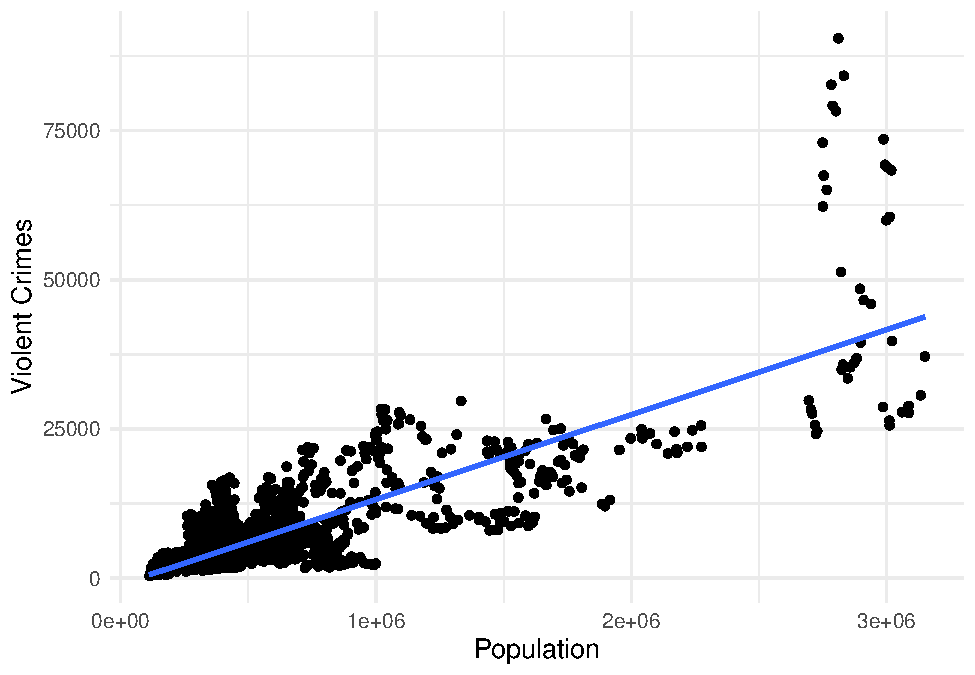
\includegraphics{_main_files/figure-latex/unnamed-chunk-75-1.pdf}

\hypertarget{pearsons-r}{%
\subsection{Pearson's r}\label{pearsons-r}}

This plot looks pretty interesting. How about calculating Pearson's r?

\begin{Shaded}
\begin{Highlighting}[]
\FunctionTok{rcorr}\NormalTok{(crime\_tidied}\SpecialCharTok{$}\NormalTok{Population, crime\_tidied}\SpecialCharTok{$}\NormalTok{Violent\_Crimes)}
\end{Highlighting}
\end{Shaded}

\begin{verbatim}
##      x    y
## x 1.00 0.81
## y 0.81 1.00
## 
## n
##      x    y
## x 1714 1708
## y 1708 1708
## 
## P
##   x  y 
## x     0
## y  0
\end{verbatim}

Look at the r and p-values - r is =.81 and p \textless{} .001. So \textasciitilde66\% of the variance in our Violent\_Crimes variable is explained by our Population size variable. Clearly there is a positive relationship between population size and the rate of violent crime. From the plot, we might conclude that the relationship is being overly influenced by crime in a small number of very large cities (top right of the plot above). Let's exclude cities with populations greater than 2,000,000

\begin{Shaded}
\begin{Highlighting}[]
\NormalTok{crime\_filtered }\OtherTok{\textless{}{-}} \FunctionTok{filter}\NormalTok{(crime\_tidied, Population }\SpecialCharTok{\textless{}} \DecValTok{2000000}\NormalTok{)}
\end{Highlighting}
\end{Shaded}

Now let's redo the plot. As there are still likely to be quite a lot of points (and thus overplotting with many points appearing roughly in the same place), we can set the alpha parameter to be \textless{} 1 in the \texttt{geom\_point()} line of code. This parameter corresponds to the translucency of each point. Change it to other values to see what happens.

\begin{Shaded}
\begin{Highlighting}[]
\NormalTok{crime\_filtered }\SpecialCharTok{\%\textgreater{}\%}
  \FunctionTok{ggplot}\NormalTok{(}\FunctionTok{aes}\NormalTok{(}\AttributeTok{x =}\NormalTok{ Population, }\AttributeTok{y =}\NormalTok{ Violent\_Crimes)) }\SpecialCharTok{+} 
  \FunctionTok{geom\_point}\NormalTok{(}\AttributeTok{alpha =}\NormalTok{ .}\DecValTok{25}\NormalTok{) }\SpecialCharTok{+} 
  \FunctionTok{geom\_smooth}\NormalTok{(}\AttributeTok{method =} \StringTok{"lm"}\NormalTok{, }\AttributeTok{se =} \ConstantTok{FALSE}\NormalTok{) }\SpecialCharTok{+}
  \FunctionTok{theme\_minimal}\NormalTok{() }\SpecialCharTok{+}
  \FunctionTok{theme}\NormalTok{(}\AttributeTok{text =} \FunctionTok{element\_text}\NormalTok{(}\AttributeTok{size =} \DecValTok{13}\NormalTok{)) }\SpecialCharTok{+}
  \FunctionTok{labs}\NormalTok{(}\AttributeTok{x =} \StringTok{"Population"}\NormalTok{, }
       \AttributeTok{y =} \StringTok{"Violent Crimes"}\NormalTok{)}
\end{Highlighting}
\end{Shaded}

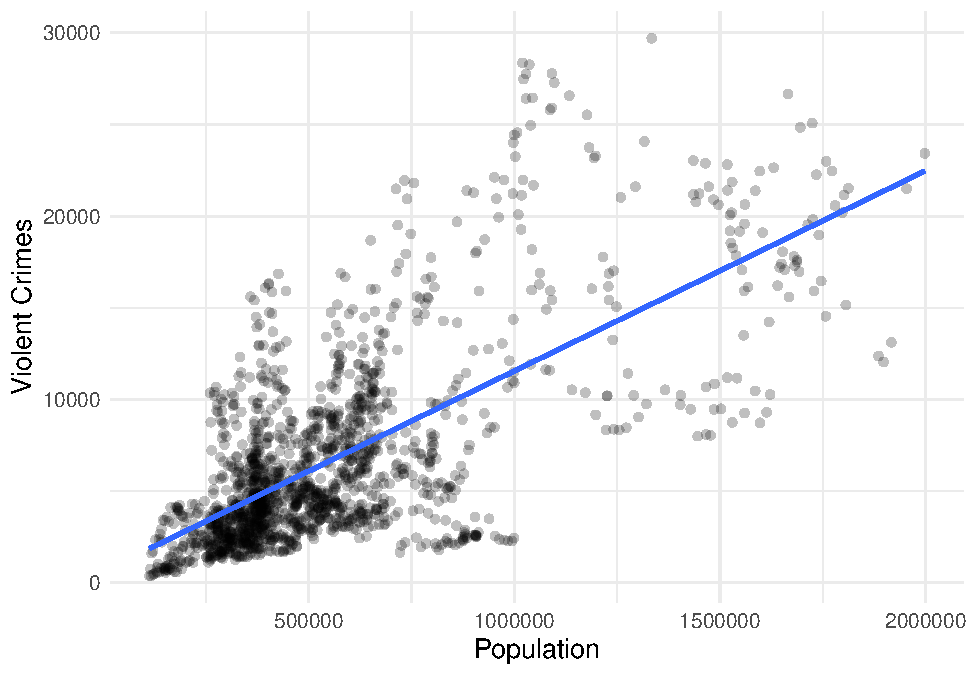
\includegraphics{_main_files/figure-latex/unnamed-chunk-78-1.pdf}

And calculate Pearson's r.

\begin{Shaded}
\begin{Highlighting}[]
\FunctionTok{rcorr}\NormalTok{(crime\_filtered}\SpecialCharTok{$}\NormalTok{Population, crime\_filtered}\SpecialCharTok{$}\NormalTok{Violent\_Crimes)}
\end{Highlighting}
\end{Shaded}

\begin{verbatim}
##      x    y
## x 1.00 0.69
## y 0.69 1.00
## 
## n
##      x    y
## x 1659 1653
## y 1653 1653
## 
## P
##   x  y 
## x     0
## y  0
\end{verbatim}

There is still a clear positive relationship (r=.69). Let's build a linear model. The dataset contains a lot of data and each city appears a number of times (once each year). For our linear model, our observations need to be independent of each other so let's just focus on the year 2015. That way each city will just appear once.

First we apply our filter.

\begin{Shaded}
\begin{Highlighting}[]
\NormalTok{crime\_filtered }\OtherTok{\textless{}{-}} \FunctionTok{filter}\NormalTok{(crime\_filtered, Year }\SpecialCharTok{==} \DecValTok{2015}\NormalTok{)}
\end{Highlighting}
\end{Shaded}

Then we build a plot. I'm using the layer \texttt{geom\_text()} to plot the City names and set the check\_overlap parameter to \texttt{TRUE} to ensure the labels don't overlap.

\begin{Shaded}
\begin{Highlighting}[]
\NormalTok{crime\_filtered }\SpecialCharTok{\%\textgreater{}\%}
  \FunctionTok{ggplot}\NormalTok{(}\FunctionTok{aes}\NormalTok{(}\AttributeTok{x =}\NormalTok{ Population, }\AttributeTok{y =}\NormalTok{ Violent\_Crimes, }\AttributeTok{label =}\NormalTok{ City)) }\SpecialCharTok{+} 
  \FunctionTok{geom\_point}\NormalTok{() }\SpecialCharTok{+} 
  \FunctionTok{geom\_text}\NormalTok{(}\AttributeTok{nudge\_y =} \DecValTok{500}\NormalTok{, }\AttributeTok{check\_overlap =} \ConstantTok{TRUE}\NormalTok{) }\SpecialCharTok{+} 
  \FunctionTok{geom\_smooth}\NormalTok{(}\AttributeTok{method =} \StringTok{"lm"}\NormalTok{, }\AttributeTok{se =} \ConstantTok{FALSE}\NormalTok{) }\SpecialCharTok{+} 
  \FunctionTok{xlim}\NormalTok{(}\DecValTok{0}\NormalTok{, }\DecValTok{1800000}\NormalTok{) }\SpecialCharTok{+}
  \FunctionTok{theme\_minimal}\NormalTok{() }\SpecialCharTok{+}
  \FunctionTok{theme}\NormalTok{(}\AttributeTok{text =} \FunctionTok{element\_text}\NormalTok{(}\AttributeTok{size =} \DecValTok{13}\NormalTok{)) }\SpecialCharTok{+}
  \FunctionTok{labs}\NormalTok{(}\AttributeTok{x =} \StringTok{"Population"}\NormalTok{, }
       \AttributeTok{y =} \StringTok{"Violent Crimes"}\NormalTok{)}
\end{Highlighting}
\end{Shaded}

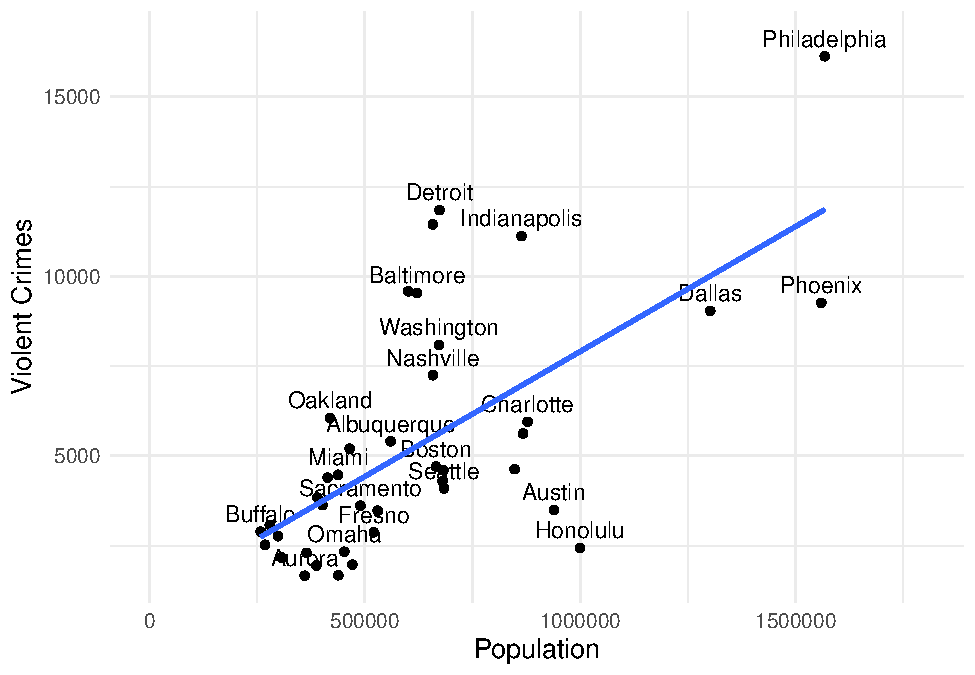
\includegraphics{_main_files/figure-latex/unnamed-chunk-81-1.pdf}

This shows a clear positive linear relationship so let's work out Pearson's r.

\begin{Shaded}
\begin{Highlighting}[]
\FunctionTok{rcorr}\NormalTok{(crime\_filtered}\SpecialCharTok{$}\NormalTok{Population, crime\_filtered}\SpecialCharTok{$}\NormalTok{Violent\_Crimes)}
\end{Highlighting}
\end{Shaded}

\begin{verbatim}
##      x    y
## x 1.00 0.65
## y 0.65 1.00
## 
## n
##    x  y
## x 42 40
## y 40 40
## 
## P
##   x  y 
## x     0
## y  0
\end{verbatim}

\hypertarget{model-the-data}{%
\subsection{Model the Data}\label{model-the-data}}

Imagine we are a city planner, and we want to know by how much we think violent crimes might increase as a function of population size. In other words, we want to work out how the violent crime rate is predicted by population size.

We're going to build two linear models - one \texttt{model1} where we're using the mean of our outcome variable as the predictor, and a second \texttt{model2} where we are using Population size to predict the Violent Crimes outcome.

\begin{Shaded}
\begin{Highlighting}[]
\NormalTok{model1 }\OtherTok{\textless{}{-}} \FunctionTok{lm}\NormalTok{(Violent\_Crimes }\SpecialCharTok{\textasciitilde{}} \DecValTok{1}\NormalTok{, }\AttributeTok{data =}\NormalTok{ crime\_filtered)}
\NormalTok{model2 }\OtherTok{\textless{}{-}} \FunctionTok{lm}\NormalTok{(Violent\_Crimes }\SpecialCharTok{\textasciitilde{}}\NormalTok{ Population, }\AttributeTok{data =}\NormalTok{ crime\_filtered)}
\end{Highlighting}
\end{Shaded}

\hypertarget{checking-our-assumptions}{%
\subsection{Checking Our Assumptions}\label{checking-our-assumptions}}

Let's use the \texttt{check\_model()} function from the performance package to check the assumptions of our model.

\begin{Shaded}
\begin{Highlighting}[]
\FunctionTok{check\_model}\NormalTok{(model2, }\AttributeTok{check =} \FunctionTok{c}\NormalTok{(}\StringTok{"homogeneity"}\NormalTok{,}\StringTok{"outliers"}\NormalTok{,}\StringTok{"qq"}\NormalTok{))}
\end{Highlighting}
\end{Shaded}

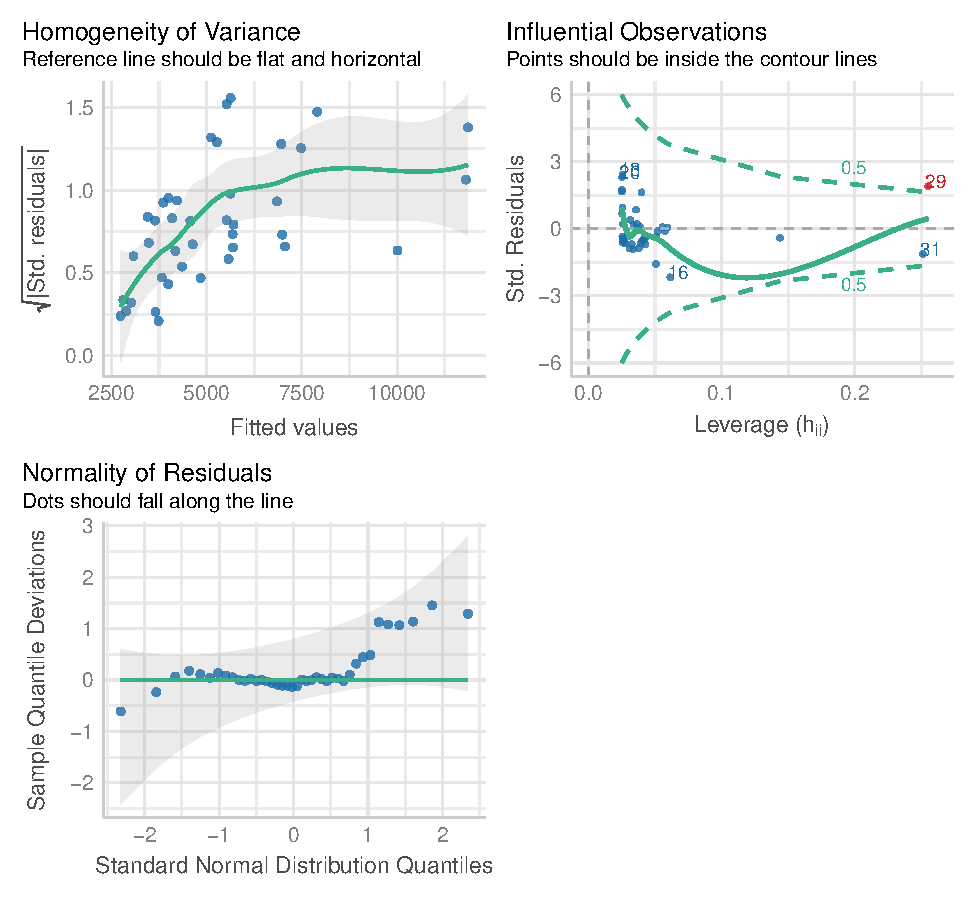
\includegraphics{_main_files/figure-latex/unnamed-chunk-84-1.pdf}

Our dataset is small and so some of our diagnostic plots don't look great. We'll come back to the influential outlier (case 29) later - but for now let's use the \texttt{anova()} function to see if our model with Population as the predictor is better than the one using just the mean.

\begin{Shaded}
\begin{Highlighting}[]
\FunctionTok{anova}\NormalTok{(model1, model2)}
\end{Highlighting}
\end{Shaded}

\begin{verbatim}
## Analysis of Variance Table
## 
## Model 1: Violent_Crimes ~ 1
## Model 2: Violent_Crimes ~ Population
##   Res.Df       RSS Df Sum of Sq      F    Pr(>F)    
## 1     39 445568991                                  
## 2     38 257690819  1 187878173 27.705 5.813e-06 ***
## ---
## Signif. codes:  0 '***' 0.001 '**' 0.01 '*' 0.05 '.' 0.1 ' ' 1
\end{verbatim}

It is - the models differ and you'll see the residual sum of squares (or the error) is less in the second model (which has Population as the predictor). This means the deviation between our observed data and the regression line model \texttt{model2} is significantly less than the deviation between our observed data and the mean as a model of our data \texttt{model1}. So let's get the parameter estimates of \texttt{model2}.

\hypertarget{interpreting-our-model}{%
\subsection{Interpreting Our Model}\label{interpreting-our-model}}

\begin{Shaded}
\begin{Highlighting}[]
\FunctionTok{summary}\NormalTok{(model2)}
\end{Highlighting}
\end{Shaded}

\begin{verbatim}
## 
## Call:
## lm(formula = Violent_Crimes ~ Population, data = crime_filtered)
## 
## Residuals:
##     Min      1Q  Median      3Q     Max 
## -5465.8 -1633.4  -809.1   684.3  6213.8 
## 
## Coefficients:
##              Estimate Std. Error t value Pr(>|t|)    
## (Intercept) 9.443e+02  9.216e+02   1.025    0.312    
## Population  6.963e-03  1.323e-03   5.264 5.81e-06 ***
## ---
## Signif. codes:  0 '***' 0.001 '**' 0.01 '*' 0.05 '.' 0.1 ' ' 1
## 
## Residual standard error: 2604 on 38 degrees of freedom
##   (2 observations deleted due to missingness)
## Multiple R-squared:  0.4217, Adjusted R-squared:  0.4064 
## F-statistic: 27.71 on 1 and 38 DF,  p-value: 5.813e-06
\end{verbatim}

The intercept corresponds to where our regression line intercepts the y-axis, and the Population parameter corresponds to the slope of our line. We see that for every increase in population by 1 there is an extra 0.006963 increase in violent crime.

For a city with a population of about a million, there will be about 7907 Violent Crimes. We calculate this by multiplying the estimate of our predictor (0.006963) by 1,000,000 and then adding the intercept (944.3). This gives us 7907.3 crimes - which tallys with what you see in our regression line above. We may have a few outliers - how would you figure out what those were? Try excluding any outliers you find and re-building your model.

\hypertarget{your-challenge-do-this-in-the-live-session-2}{%
\subsection{Your Challenge (do this in the live session)}\label{your-challenge-do-this-in-the-live-session-2}}

You now have three tasks:
1. Check whether the same relationship holds for population size and robberies in 2015.
2. Are house prices predicted by the number of violent crimes in 2015?
3. Are house prices predicted by population size in 2015?

\textbf{End of workshop 6 materials}

\hypertarget{regression-part-2}{%
\chapter{Regression Part 2}\label{regression-part-2}}

In this workshop we will explore Multiple Regression in the context of the General Linear Model (GLM). Multiple Regression builds on Simple Regression, except that instead of having one predictor (as is the case with Simple Regression) we will be dealing with multiple predictors. Again, you will have the opportunity to build some regression models and use various methods to decide which one is `best'. You will also learn how to run model diagnostics for these models as you did in the case of Simple Regression.

\hypertarget{overview-2}{%
\section{Overview}\label{overview-2}}

First off I'd like you to watch the following video which builds on the first regression workshop. We explore how to build regression models with more than one predictor in R using the \texttt{lm()} function, test our model assumptions, and interpret the output. We look at different ways of building stepwise regression models with multiple predictors, before finishing by looking at mediation and moderation.

~~

~~

\hypertarget{multiple-regression}{%
\section{Multiple Regression}\label{multiple-regression}}

In standard multiple regression all the independent variables (IVs) are entered into the equation and evaluated for their contribution at the same time. Let's work through a specific example.

An educational psychologist conducted a study that investigated the psycholinguistic variables that contribute to spelling performance in primary school children aged between 7- and 9-years. The researcher presented children with 48 words that varied systematically according to certain features such as age of acquisition, word frequency, word length, and imageability. The psychologist wants to check whether performance on the test accurately reflected children's spelling ability as estimated by a standardised spelling test. That is, the psychologist wants to check whether her test was appropriate.

Children's chronological age (in months) (age), their reading age (RA), their standardised reading age (std\_RA), and their standardised spelling score (std\_SPELL) were chosen as predictor variables. The criterion variable (Y) was the percentage correct spelling (corr\_spell) score attained by each child using the list of 48 words.

First we need to load the packages we need - the require function assumes they are already on your machine. If they are not, then you need to install.packages (``packagename'') first:

\hypertarget{the-packages-we-need-1}{%
\subsection{The Packages We Need}\label{the-packages-we-need-1}}

\begin{Shaded}
\begin{Highlighting}[]
\FunctionTok{library}\NormalTok{(tidyverse) }\CommentTok{\# Load the tidyverse packages}
\FunctionTok{library}\NormalTok{(Hmisc) }\CommentTok{\# Needed for correlation}
\FunctionTok{library}\NormalTok{(MASS) }\CommentTok{\# Needed for maths functions}
\FunctionTok{library}\NormalTok{(car) }\CommentTok{\# Needed for VIF calculation}
\FunctionTok{library}\NormalTok{(olsrr) }\CommentTok{\# Needed for stepwise regression }
\FunctionTok{library}\NormalTok{(performance) }\CommentTok{\# Needed to check model assumptions}
\end{Highlighting}
\end{Shaded}

\hypertarget{import-the-data-1}{%
\subsection{Import the Data}\label{import-the-data-1}}

You now need to read in the data file.

\begin{Shaded}
\begin{Highlighting}[]
\NormalTok{MRes\_tut2 }\OtherTok{\textless{}{-}} \FunctionTok{read\_csv}\NormalTok{(}\StringTok{"https://raw.githubusercontent.com/ajstewartlang/10\_glm\_regression\_pt2/master/data/MRes\_tut2.csv"}\NormalTok{)}
\end{Highlighting}
\end{Shaded}

\hypertarget{examining-possible-relationships}{%
\subsubsection*{Examining Possible Relationships}\label{examining-possible-relationships}}
\addcontentsline{toc}{subsubsection}{Examining Possible Relationships}

Before we start, let's look at the relationships between our IVs (predictors) and our DV (outcome). We can plot graphs depicting the correlations. We'll plot test performance against each of our four predictors in turn:

\begin{Shaded}
\begin{Highlighting}[]
\FunctionTok{ggplot}\NormalTok{(MRes\_tut2, }\FunctionTok{aes}\NormalTok{(}\AttributeTok{x =}\NormalTok{ age, }\AttributeTok{y =}\NormalTok{ corr\_spell)) }\SpecialCharTok{+} 
  \FunctionTok{geom\_point}\NormalTok{() }\SpecialCharTok{+} 
  \FunctionTok{geom\_smooth}\NormalTok{(}\AttributeTok{method =} \StringTok{"lm"}\NormalTok{, }\AttributeTok{se =} \ConstantTok{FALSE}\NormalTok{) }\SpecialCharTok{+}
  \FunctionTok{theme\_minimal}\NormalTok{() }\SpecialCharTok{+}
  \FunctionTok{theme}\NormalTok{(}\AttributeTok{text =} \FunctionTok{element\_text}\NormalTok{(}\AttributeTok{size =} \DecValTok{13}\NormalTok{)) }
\end{Highlighting}
\end{Shaded}

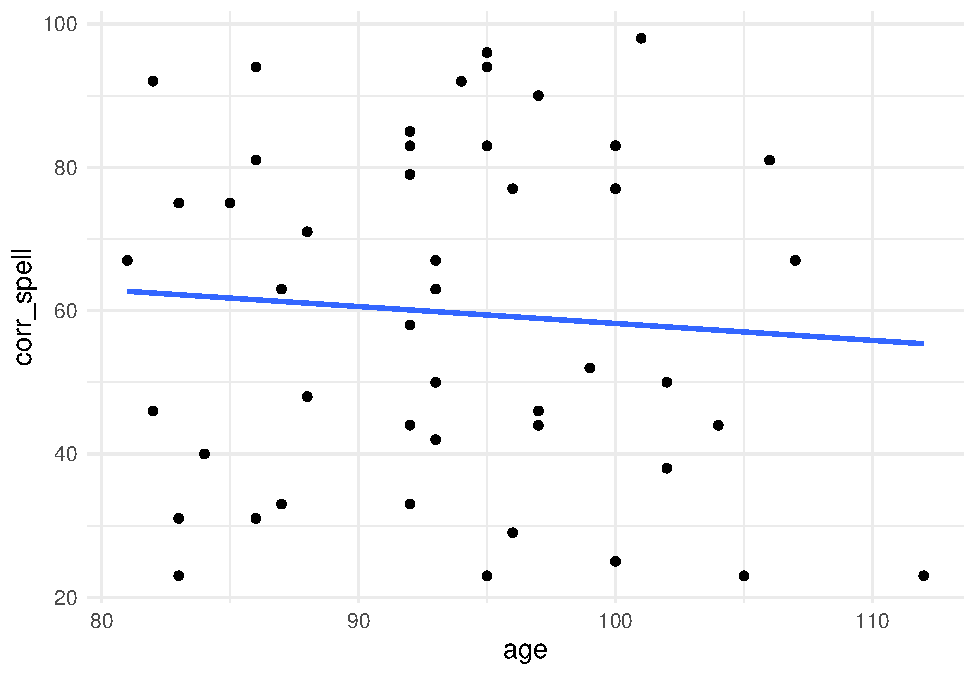
\includegraphics{_main_files/figure-latex/unnamed-chunk-89-1.pdf}

\begin{Shaded}
\begin{Highlighting}[]
\FunctionTok{ggplot}\NormalTok{(MRes\_tut2, }\FunctionTok{aes}\NormalTok{(}\AttributeTok{x =}\NormalTok{ RA, }\AttributeTok{y =}\NormalTok{ corr\_spell)) }\SpecialCharTok{+} 
  \FunctionTok{geom\_point}\NormalTok{() }\SpecialCharTok{+} 
  \FunctionTok{geom\_smooth}\NormalTok{(}\AttributeTok{method =} \StringTok{"lm"}\NormalTok{, }\AttributeTok{se =} \ConstantTok{FALSE}\NormalTok{) }\SpecialCharTok{+}
  \FunctionTok{theme\_minimal}\NormalTok{() }\SpecialCharTok{+}
  \FunctionTok{theme}\NormalTok{(}\AttributeTok{text =} \FunctionTok{element\_text}\NormalTok{(}\AttributeTok{size =} \DecValTok{13}\NormalTok{)) }
\end{Highlighting}
\end{Shaded}

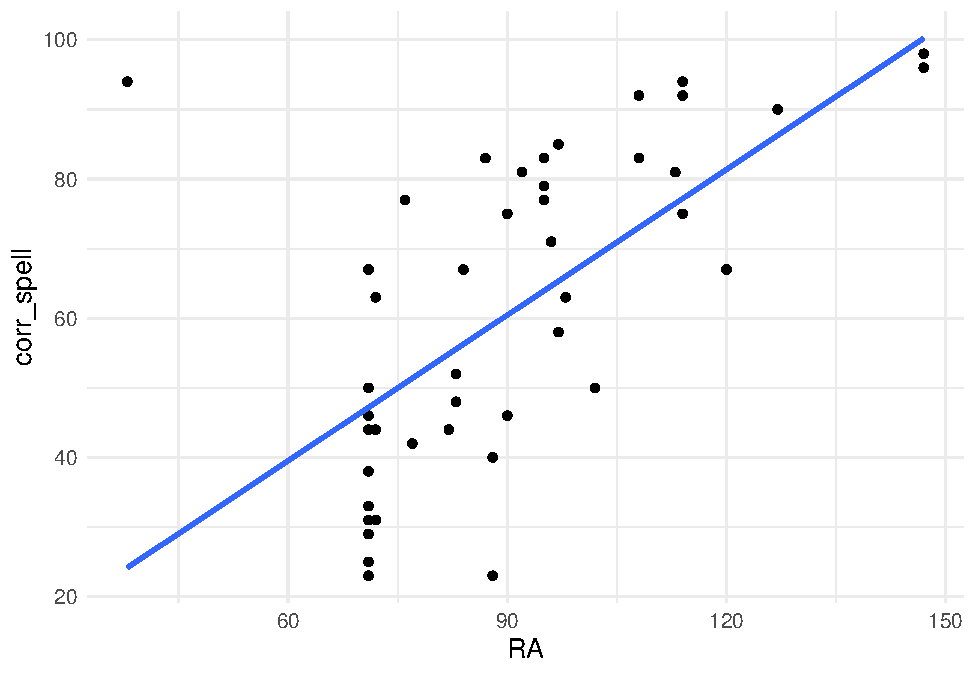
\includegraphics{_main_files/figure-latex/unnamed-chunk-89-2.pdf}

\begin{Shaded}
\begin{Highlighting}[]
\FunctionTok{ggplot}\NormalTok{(MRes\_tut2, }\FunctionTok{aes}\NormalTok{(}\AttributeTok{x =}\NormalTok{ std\_RA, }\AttributeTok{y =}\NormalTok{ corr\_spell)) }\SpecialCharTok{+} 
  \FunctionTok{geom\_point}\NormalTok{() }\SpecialCharTok{+} 
  \FunctionTok{geom\_smooth}\NormalTok{(}\AttributeTok{method =} \StringTok{"lm"}\NormalTok{, }\AttributeTok{se =} \ConstantTok{FALSE}\NormalTok{) }\SpecialCharTok{+}
  \FunctionTok{theme\_minimal}\NormalTok{() }\SpecialCharTok{+}
  \FunctionTok{theme}\NormalTok{(}\AttributeTok{text =} \FunctionTok{element\_text}\NormalTok{(}\AttributeTok{size =} \DecValTok{13}\NormalTok{)) }
\end{Highlighting}
\end{Shaded}

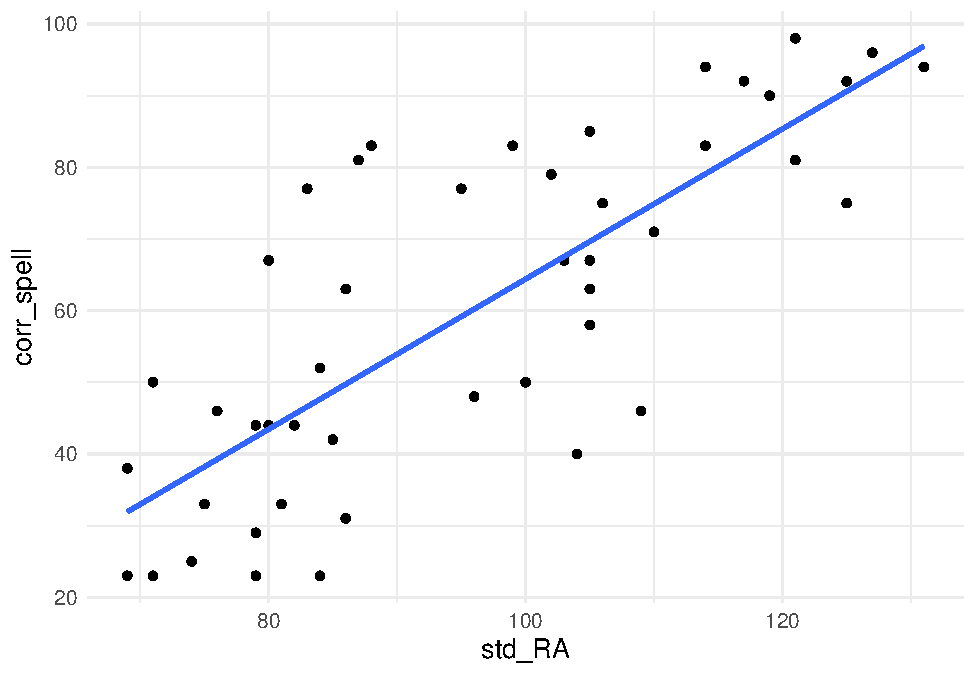
\includegraphics{_main_files/figure-latex/unnamed-chunk-89-3.pdf}

\begin{Shaded}
\begin{Highlighting}[]
\FunctionTok{ggplot}\NormalTok{(MRes\_tut2, }\FunctionTok{aes}\NormalTok{(}\AttributeTok{x =}\NormalTok{ std\_SPELL, }\AttributeTok{y =}\NormalTok{ corr\_spell)) }\SpecialCharTok{+} 
  \FunctionTok{geom\_point}\NormalTok{() }\SpecialCharTok{+} 
  \FunctionTok{geom\_smooth}\NormalTok{(}\AttributeTok{method =} \StringTok{"lm"}\NormalTok{, }\AttributeTok{se =} \ConstantTok{FALSE}\NormalTok{) }\SpecialCharTok{+}
  \FunctionTok{theme\_minimal}\NormalTok{() }\SpecialCharTok{+}
  \FunctionTok{theme}\NormalTok{(}\AttributeTok{text =} \FunctionTok{element\_text}\NormalTok{(}\AttributeTok{size =} \DecValTok{13}\NormalTok{)) }
\end{Highlighting}
\end{Shaded}

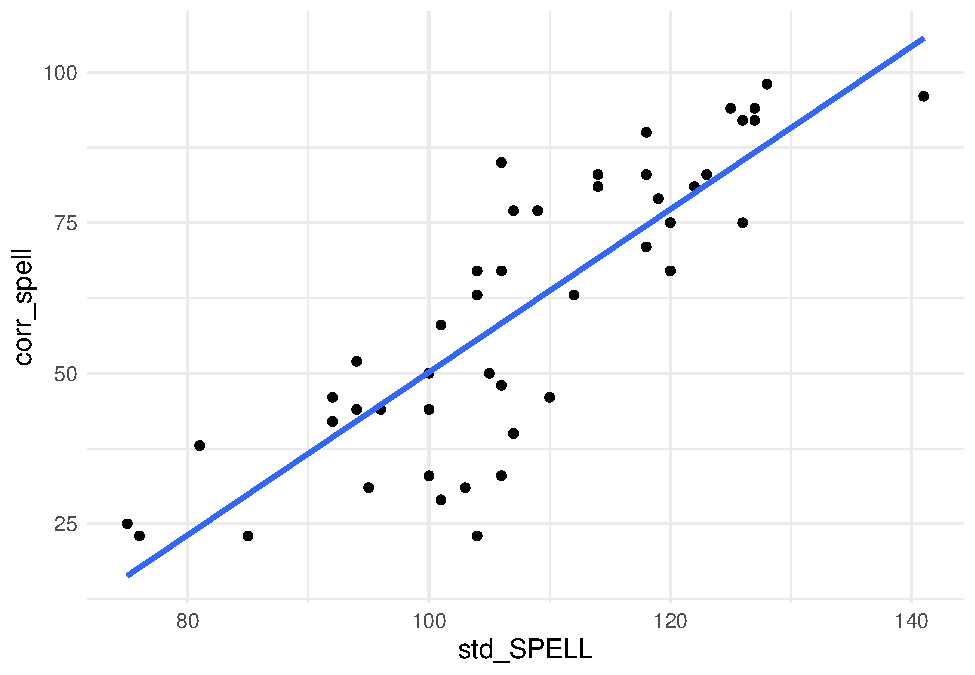
\includegraphics{_main_files/figure-latex/unnamed-chunk-89-4.pdf}

\hypertarget{model-the-data-1}{%
\subsection{Model the Data}\label{model-the-data-1}}

We are going to do hierarchical regression first - we'll build one model (which we'll call \texttt{model0}) that is the mean of our outcome variable, and another model (\texttt{model1}) which contains all our predictors:

\begin{Shaded}
\begin{Highlighting}[]
\NormalTok{model0 }\OtherTok{\textless{}{-}} \FunctionTok{lm}\NormalTok{(corr\_spell }\SpecialCharTok{\textasciitilde{}} \DecValTok{1}\NormalTok{, }\AttributeTok{data =}\NormalTok{ MRes\_tut2)}
\NormalTok{model1 }\OtherTok{\textless{}{-}} \FunctionTok{lm}\NormalTok{(corr\_spell }\SpecialCharTok{\textasciitilde{}}\NormalTok{ age }\SpecialCharTok{+}\NormalTok{ RA }\SpecialCharTok{+}\NormalTok{ std\_RA }\SpecialCharTok{+}\NormalTok{ std\_SPELL, }\AttributeTok{data =}\NormalTok{ MRes\_tut2)}
\end{Highlighting}
\end{Shaded}

Let's compare them to each other:

\begin{Shaded}
\begin{Highlighting}[]
\FunctionTok{anova}\NormalTok{(model0, model1)}
\end{Highlighting}
\end{Shaded}

\begin{verbatim}
## Analysis of Variance Table
## 
## Model 1: corr_spell ~ 1
## Model 2: corr_spell ~ age + RA + std_RA + std_SPELL
##   Res.Df     RSS Df Sum of Sq      F    Pr(>F)    
## 1     46 26348.4                                  
## 2     42  3901.1  4     22447 60.417 < 2.2e-16 ***
## ---
## Signif. codes:  0 '***' 0.001 '**' 0.01 '*' 0.05 '.' 0.1 ' ' 1
\end{verbatim}

We see that the models differ from each other (look a the \emph{p}-value of the comparison) and that the model with the four predictors has the lower Residuals (RSS) value meaning there is less error between the model and the observed data relative to the simpler intercept-only model (i.e., the mean) and the observed data.

\hypertarget{checking-our-assumptions-1}{%
\subsubsection*{Checking our Assumptions}\label{checking-our-assumptions-1}}
\addcontentsline{toc}{subsubsection}{Checking our Assumptions}

OK, so they differ - now let's plot information about our model assumptions - remember, we are particularly interested in Cook's distance values for our case\ldots{}

\begin{Shaded}
\begin{Highlighting}[]
\FunctionTok{check\_model}\NormalTok{(model1, }\AttributeTok{check =} \FunctionTok{c}\NormalTok{(}\StringTok{"homogeneity"}\NormalTok{,}\StringTok{"outliers"}\NormalTok{,}\StringTok{"qq"}\NormalTok{,}\StringTok{"vif"}\NormalTok{))}
\end{Highlighting}
\end{Shaded}

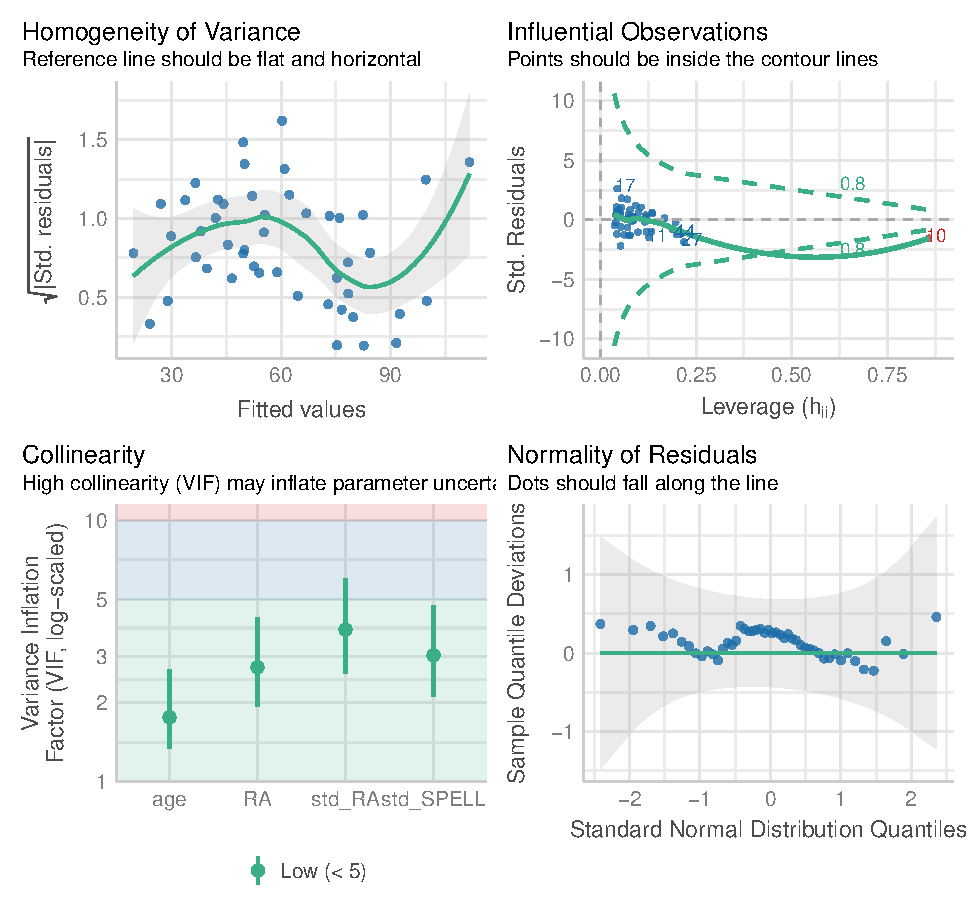
\includegraphics{_main_files/figure-latex/unnamed-chunk-92-1.pdf}

The errors looks fairly equally distributed along our fitted values (homogeneity of variance) - although a little worse for high fitted values - and from the Q-Q plot we can tell they look fairly normal (they should follow the diagonal). How about influential cases? So, Case 10 looks a bit dodgy - it has a high Cook's Distance value (indicated by it falling outside of the dashed lines) - which suggests it is having a disproportionate effect on our model. Let's exclude it using the \texttt{filter()} function - the symbol \texttt{!=} means `does not equal' so we are selecting values other than Case 10.

\hypertarget{dropping-an-influential-case}{%
\subsubsection*{Dropping an Influential Case}\label{dropping-an-influential-case}}
\addcontentsline{toc}{subsubsection}{Dropping an Influential Case}

\begin{Shaded}
\begin{Highlighting}[]
\NormalTok{MRes\_tut2\_drop10 }\OtherTok{\textless{}{-}} \FunctionTok{filter}\NormalTok{(MRes\_tut2, case }\SpecialCharTok{!=} \StringTok{"10"}\NormalTok{)}
\end{Highlighting}
\end{Shaded}

\hypertarget{remodel-the-data}{%
\subsubsection*{Re(model) the Data}\label{remodel-the-data}}
\addcontentsline{toc}{subsubsection}{Re(model) the Data}

We now create another model (\texttt{model2}) which doesn't include Case 10.

\begin{Shaded}
\begin{Highlighting}[]
\NormalTok{model2 }\OtherTok{\textless{}{-}} \FunctionTok{lm}\NormalTok{(corr\_spell }\SpecialCharTok{\textasciitilde{}}\NormalTok{ age }\SpecialCharTok{+}\NormalTok{ RA }\SpecialCharTok{+}\NormalTok{ std\_RA }\SpecialCharTok{+}\NormalTok{ std\_SPELL, }\AttributeTok{data =}\NormalTok{ MRes\_tut2\_drop10)}
\end{Highlighting}
\end{Shaded}

Let's check the model assumptions again using \texttt{check\_model()}.

\hypertarget{checking-our-assumptions-2}{%
\subsubsection*{Checking our Assumptions}\label{checking-our-assumptions-2}}
\addcontentsline{toc}{subsubsection}{Checking our Assumptions}

\begin{Shaded}
\begin{Highlighting}[]
\FunctionTok{check\_model}\NormalTok{(model2, }\AttributeTok{check =} \FunctionTok{c}\NormalTok{(}\StringTok{"homogeneity"}\NormalTok{,}\StringTok{"outliers"}\NormalTok{,}\StringTok{"qq"}\NormalTok{,}\StringTok{"vif"}\NormalTok{))}
\end{Highlighting}
\end{Shaded}

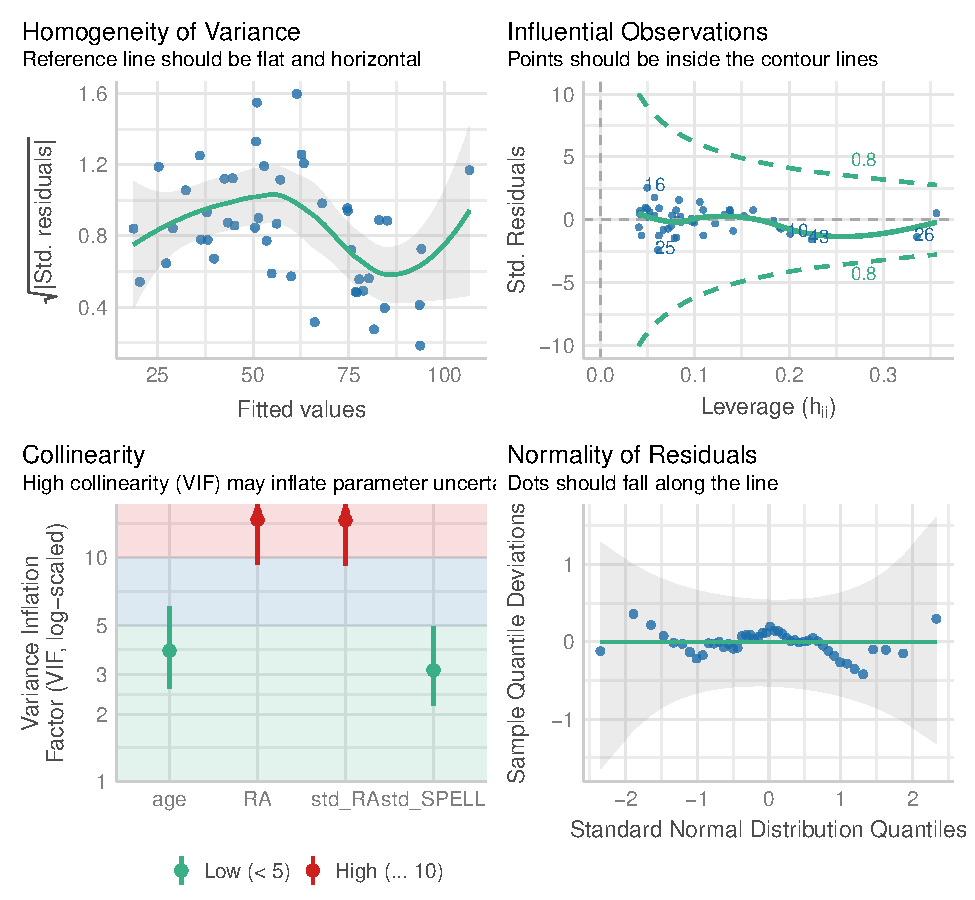
\includegraphics{_main_files/figure-latex/unnamed-chunk-95-1.pdf}

Now, let's look at the multicollinearity values measured by VIF:

\begin{Shaded}
\begin{Highlighting}[]
\FunctionTok{vif}\NormalTok{(model2)}
\end{Highlighting}
\end{Shaded}

\begin{verbatim}
##       age        RA    std_RA std_SPELL 
##  3.843462 14.763168 14.672084  3.140457
\end{verbatim}

It looks like RA and std\_RA are problematic. We can look at the correlation between them using the \texttt{rcorr()} function:

\begin{Shaded}
\begin{Highlighting}[]
\FunctionTok{rcorr}\NormalTok{(MRes\_tut2\_drop10}\SpecialCharTok{$}\NormalTok{RA, MRes\_tut2\_drop10}\SpecialCharTok{$}\NormalTok{std\_RA)}
\end{Highlighting}
\end{Shaded}

\begin{verbatim}
##      x    y
## x 1.00 0.88
## y 0.88 1.00
## 
## n= 46 
## 
## 
## P
##   x  y 
## x     0
## y  0
\end{verbatim}

\hypertarget{remodel-the-data-1}{%
\subsubsection*{Re(model) the Data}\label{remodel-the-data-1}}
\addcontentsline{toc}{subsubsection}{Re(model) the Data}

The correlation is pretty high (0.88), so let's exclude the predictor with the highest VIF value (which is RA) and build a new model:

\begin{Shaded}
\begin{Highlighting}[]
\NormalTok{model3 }\OtherTok{\textless{}{-}} \FunctionTok{lm}\NormalTok{(corr\_spell }\SpecialCharTok{\textasciitilde{}}\NormalTok{ age }\SpecialCharTok{+}\NormalTok{ std\_RA }\SpecialCharTok{+}\NormalTok{ std\_SPELL, }\AttributeTok{data =}\NormalTok{ MRes\_tut2\_drop10)}
\FunctionTok{vif}\NormalTok{(model3)}
\end{Highlighting}
\end{Shaded}

\begin{verbatim}
##       age    std_RA std_SPELL 
##  1.190827  2.636186  2.821235
\end{verbatim}

\hypertarget{checking-our-assumptions-3}{%
\subsubsection*{Checking our Assumptions}\label{checking-our-assumptions-3}}
\addcontentsline{toc}{subsubsection}{Checking our Assumptions}

These values look ok now. Let's check the model assumptions again.

\begin{Shaded}
\begin{Highlighting}[]
\FunctionTok{check\_model}\NormalTok{(model3, }\AttributeTok{check =} \FunctionTok{c}\NormalTok{(}\StringTok{"homogeneity"}\NormalTok{,}\StringTok{"outliers"}\NormalTok{,}\StringTok{"qq"}\NormalTok{,}\StringTok{"vif"}\NormalTok{))}
\end{Highlighting}
\end{Shaded}

\includegraphics{_main_files/figure-latex/unnamed-chunk-99-1.pdf}

\hypertarget{summary-of-our-model}{%
\subsubsection*{Summary of our Model}\label{summary-of-our-model}}
\addcontentsline{toc}{subsubsection}{Summary of our Model}

Now let's generate the coefficients as this looks like a sensible model.

\begin{Shaded}
\begin{Highlighting}[]
\FunctionTok{summary}\NormalTok{(model3)}
\end{Highlighting}
\end{Shaded}

\begin{verbatim}
## 
## Call:
## lm(formula = corr_spell ~ age + std_RA + std_SPELL, data = MRes_tut2_drop10)
## 
## Residuals:
##     Min      1Q  Median      3Q     Max 
## -19.801  -6.907   1.327   5.155  24.669 
## 
## Coefficients:
##              Estimate Std. Error t value Pr(>|t|)    
## (Intercept) -209.4400    26.7210  -7.838 9.43e-10 ***
## age            1.1033     0.2133   5.172 6.09e-06 ***
## std_RA         0.3804     0.1385   2.747  0.00883 ** 
## std_SPELL      1.2107     0.1650   7.339 4.78e-09 ***
## ---
## Signif. codes:  0 '***' 0.001 '**' 0.01 '*' 0.05 '.' 0.1 ' ' 1
## 
## Residual standard error: 9.824 on 42 degrees of freedom
## Multiple R-squared:  0.8388, Adjusted R-squared:  0.8273 
## F-statistic: 72.87 on 3 and 42 DF,  p-value: < 2.2e-16
\end{verbatim}

\begin{Shaded}
\begin{Highlighting}[]
\NormalTok{model0 }\OtherTok{\textless{}{-}} \FunctionTok{lm}\NormalTok{(corr\_spell }\SpecialCharTok{\textasciitilde{}} \DecValTok{1}\NormalTok{, }\AttributeTok{data =}\NormalTok{ MRes\_tut2\_drop10)}
\FunctionTok{anova}\NormalTok{(model3, model0)}
\end{Highlighting}
\end{Shaded}

\begin{verbatim}
## Analysis of Variance Table
## 
## Model 1: corr_spell ~ age + std_RA + std_SPELL
## Model 2: corr_spell ~ 1
##   Res.Df     RSS Df Sum of Sq      F    Pr(>F)    
## 1     42  4053.5                                  
## 2     45 25151.0 -3    -21098 72.866 < 2.2e-16 ***
## ---
## Signif. codes:  0 '***' 0.001 '**' 0.01 '*' 0.05 '.' 0.1 ' ' 1
\end{verbatim}

We'd write our equation as something like:

\texttt{Spelled\ correct\ =\ -209.44\ +\ 1.10(age)\ +\ 0.38(std\_RA)\ +\ 1.21(std\_SPELL)\ +\ residual}

\hypertarget{stepwise-regression}{%
\section{Stepwise regression}\label{stepwise-regression}}

We can also do stepwise regression - forwards is when you start with the null model and predictors are added until they don't explain any more variance, backwards is when you start with the full model and remove predictors until removal starts affecting your model's predictive ability. Let's keep case 10 dropped and also drop the high VIF predictor (RA). This is handy for models with lots of predictors where the order in sequential regression is not obvious.

\hypertarget{model-the-data-2}{%
\subsection{Model the Data}\label{model-the-data-2}}

\begin{Shaded}
\begin{Highlighting}[]
\NormalTok{model0 }\OtherTok{\textless{}{-}} \FunctionTok{lm}\NormalTok{(corr\_spell }\SpecialCharTok{\textasciitilde{}} \DecValTok{1}\NormalTok{, }\AttributeTok{data =}\NormalTok{ MRes\_tut2\_drop10)}
\NormalTok{model1 }\OtherTok{\textless{}{-}} \FunctionTok{lm}\NormalTok{(corr\_spell }\SpecialCharTok{\textasciitilde{}}\NormalTok{ age }\SpecialCharTok{+}\NormalTok{ std\_RA }\SpecialCharTok{+}\NormalTok{ std\_SPELL, }\AttributeTok{data =}\NormalTok{ MRes\_tut2\_drop10)}
\end{Highlighting}
\end{Shaded}

Let's do stepwise forwards:

\begin{Shaded}
\begin{Highlighting}[]
\NormalTok{steplimitsf }\OtherTok{\textless{}{-}} \FunctionTok{step}\NormalTok{(model0, }\AttributeTok{scope =} \FunctionTok{list}\NormalTok{ (}\AttributeTok{lower =}\NormalTok{ model0, }\AttributeTok{upper =}\NormalTok{ model1), }\AttributeTok{direction =} \StringTok{"forward"}\NormalTok{)}
\end{Highlighting}
\end{Shaded}

\begin{verbatim}
## Start:  AIC=291.98
## corr_spell ~ 1
## 
##             Df Sum of Sq     RSS    AIC
## + std_SPELL  1   17802.2  7348.8 237.39
## + std_RA     1   14780.1 10370.9 253.23
## <none>                   25151.0 291.98
## + age        1      48.7 25102.3 293.89
## 
## Step:  AIC=237.39
## corr_spell ~ std_SPELL
## 
##          Df Sum of Sq    RSS    AIC
## + age     1   2567.20 4781.6 219.62
## + std_RA  1    714.14 6634.7 234.69
## <none>                7348.8 237.39
## 
## Step:  AIC=219.62
## corr_spell ~ std_SPELL + age
## 
##          Df Sum of Sq    RSS    AIC
## + std_RA  1     728.1 4053.5 214.02
## <none>                4781.6 219.62
## 
## Step:  AIC=214.02
## corr_spell ~ std_SPELL + age + std_RA
\end{verbatim}

\begin{Shaded}
\begin{Highlighting}[]
\FunctionTok{summary}\NormalTok{(steplimitsf)}
\end{Highlighting}
\end{Shaded}

\begin{verbatim}
## 
## Call:
## lm(formula = corr_spell ~ std_SPELL + age + std_RA, data = MRes_tut2_drop10)
## 
## Residuals:
##     Min      1Q  Median      3Q     Max 
## -19.801  -6.907   1.327   5.155  24.669 
## 
## Coefficients:
##              Estimate Std. Error t value Pr(>|t|)    
## (Intercept) -209.4400    26.7210  -7.838 9.43e-10 ***
## std_SPELL      1.2107     0.1650   7.339 4.78e-09 ***
## age            1.1033     0.2133   5.172 6.09e-06 ***
## std_RA         0.3804     0.1385   2.747  0.00883 ** 
## ---
## Signif. codes:  0 '***' 0.001 '**' 0.01 '*' 0.05 '.' 0.1 ' ' 1
## 
## Residual standard error: 9.824 on 42 degrees of freedom
## Multiple R-squared:  0.8388, Adjusted R-squared:  0.8273 
## F-statistic: 72.87 on 3 and 42 DF,  p-value: < 2.2e-16
\end{verbatim}

Stepwise backwards:

\begin{Shaded}
\begin{Highlighting}[]
\NormalTok{steplimitsb }\OtherTok{\textless{}{-}} \FunctionTok{step}\NormalTok{(model1, }\AttributeTok{direction =} \StringTok{"back"}\NormalTok{)}
\end{Highlighting}
\end{Shaded}

\begin{verbatim}
## Start:  AIC=214.02
## corr_spell ~ age + std_RA + std_SPELL
## 
##             Df Sum of Sq    RSS    AIC
## <none>                   4053.5 214.02
## - std_RA     1     728.1 4781.6 219.62
## - age        1    2581.2 6634.7 234.69
## - std_SPELL  1    5198.3 9251.8 249.98
\end{verbatim}

\begin{Shaded}
\begin{Highlighting}[]
\FunctionTok{summary}\NormalTok{(steplimitsb)}
\end{Highlighting}
\end{Shaded}

\begin{verbatim}
## 
## Call:
## lm(formula = corr_spell ~ age + std_RA + std_SPELL, data = MRes_tut2_drop10)
## 
## Residuals:
##     Min      1Q  Median      3Q     Max 
## -19.801  -6.907   1.327   5.155  24.669 
## 
## Coefficients:
##              Estimate Std. Error t value Pr(>|t|)    
## (Intercept) -209.4400    26.7210  -7.838 9.43e-10 ***
## age            1.1033     0.2133   5.172 6.09e-06 ***
## std_RA         0.3804     0.1385   2.747  0.00883 ** 
## std_SPELL      1.2107     0.1650   7.339 4.78e-09 ***
## ---
## Signif. codes:  0 '***' 0.001 '**' 0.01 '*' 0.05 '.' 0.1 ' ' 1
## 
## Residual standard error: 9.824 on 42 degrees of freedom
## Multiple R-squared:  0.8388, Adjusted R-squared:  0.8273 
## F-statistic: 72.87 on 3 and 42 DF,  p-value: < 2.2e-16
\end{verbatim}

And stepwise using both forwards and backwards procedures:

\begin{Shaded}
\begin{Highlighting}[]
\NormalTok{steplimitsboth }\OtherTok{\textless{}{-}} \FunctionTok{step}\NormalTok{(model0, }\AttributeTok{scope =} \FunctionTok{list}\NormalTok{ (}\AttributeTok{upper =}\NormalTok{ model1), }\AttributeTok{direction =} \StringTok{"both"}\NormalTok{)}
\end{Highlighting}
\end{Shaded}

\begin{verbatim}
## Start:  AIC=291.98
## corr_spell ~ 1
## 
##             Df Sum of Sq     RSS    AIC
## + std_SPELL  1   17802.2  7348.8 237.39
## + std_RA     1   14780.1 10370.9 253.23
## <none>                   25151.0 291.98
## + age        1      48.7 25102.3 293.89
## 
## Step:  AIC=237.39
## corr_spell ~ std_SPELL
## 
##             Df Sum of Sq     RSS    AIC
## + age        1    2567.2  4781.6 219.62
## + std_RA     1     714.1  6634.7 234.69
## <none>                    7348.8 237.39
## - std_SPELL  1   17802.2 25151.0 291.98
## 
## Step:  AIC=219.62
## corr_spell ~ std_SPELL + age
## 
##             Df Sum of Sq     RSS    AIC
## + std_RA     1     728.1  4053.5 214.02
## <none>                    4781.6 219.62
## - age        1    2567.2  7348.8 237.39
## - std_SPELL  1   20320.7 25102.3 293.89
## 
## Step:  AIC=214.02
## corr_spell ~ std_SPELL + age + std_RA
## 
##             Df Sum of Sq    RSS    AIC
## <none>                   4053.5 214.02
## - std_RA     1     728.1 4781.6 219.62
## - age        1    2581.2 6634.7 234.69
## - std_SPELL  1    5198.3 9251.8 249.98
\end{verbatim}

\hypertarget{checking-our-assumptions-4}{%
\subsubsection*{Checking our Assumptions}\label{checking-our-assumptions-4}}
\addcontentsline{toc}{subsubsection}{Checking our Assumptions}

\begin{Shaded}
\begin{Highlighting}[]
\FunctionTok{check\_model}\NormalTok{(steplimitsboth, }\AttributeTok{check =} \FunctionTok{c}\NormalTok{(}\StringTok{"homogeneity"}\NormalTok{,}\StringTok{"outliers"}\NormalTok{,}\StringTok{"qq"}\NormalTok{,}\StringTok{"vif"}\NormalTok{))}
\end{Highlighting}
\end{Shaded}

\includegraphics{_main_files/figure-latex/unnamed-chunk-105-1.pdf}

These look ok.

\begin{Shaded}
\begin{Highlighting}[]
\FunctionTok{summary}\NormalTok{(steplimitsboth)}
\end{Highlighting}
\end{Shaded}

\begin{verbatim}
## 
## Call:
## lm(formula = corr_spell ~ std_SPELL + age + std_RA, data = MRes_tut2_drop10)
## 
## Residuals:
##     Min      1Q  Median      3Q     Max 
## -19.801  -6.907   1.327   5.155  24.669 
## 
## Coefficients:
##              Estimate Std. Error t value Pr(>|t|)    
## (Intercept) -209.4400    26.7210  -7.838 9.43e-10 ***
## std_SPELL      1.2107     0.1650   7.339 4.78e-09 ***
## age            1.1033     0.2133   5.172 6.09e-06 ***
## std_RA         0.3804     0.1385   2.747  0.00883 ** 
## ---
## Signif. codes:  0 '***' 0.001 '**' 0.01 '*' 0.05 '.' 0.1 ' ' 1
## 
## Residual standard error: 9.824 on 42 degrees of freedom
## Multiple R-squared:  0.8388, Adjusted R-squared:  0.8273 
## F-statistic: 72.87 on 3 and 42 DF,  p-value: < 2.2e-16
\end{verbatim}

You'll see that the same final model is arrived it in each case. We have three significant predictors.

\hypertarget{entering-predictors-based-on-their-p-values}{%
\subsubsection*{\texorpdfstring{Entering predictors based on their \emph{p}-values}{Entering predictors based on their p-values}}\label{entering-predictors-based-on-their-p-values}}
\addcontentsline{toc}{subsubsection}{Entering predictors based on their \emph{p}-values}

We can also use the \texttt{ols\_step\_forward\_p()} function from the package \texttt{olsrr} - this works by finding the best model by entering the predictors based on their \emph{p} values. There are other methods within the \texttt{olsrr} package. To see them, type \texttt{olsrr::} into the console window.

\begin{Shaded}
\begin{Highlighting}[]
\NormalTok{pmodel }\OtherTok{\textless{}{-}} \FunctionTok{ols\_step\_forward\_p}\NormalTok{(model1)}
\NormalTok{pmodel}
\end{Highlighting}
\end{Shaded}

\begin{verbatim}
## 
##                              Selection Summary                              
## ---------------------------------------------------------------------------
##         Variable                   Adj.                                        
## Step     Entered     R-Square    R-Square     C(p)        AIC        RMSE      
## ---------------------------------------------------------------------------
##    1    std_SPELL      0.7078      0.7012    34.1439    369.9304    12.9236    
##    2    age            0.8099      0.8010     9.5442    352.1614    10.5452    
##    3    std_RA         0.8388      0.8273     4.0000    346.5624     9.8241    
## ---------------------------------------------------------------------------
\end{verbatim}

In this case, the model with the lowest AIC value is also the one arrived at statistically via the sequential procedure based on \emph{p}-values - but this may not always be the case.

\textbf{End of workshop 7 materials}

\hypertarget{anova-part-1}{%
\chapter{ANOVA Part 1}\label{anova-part-1}}

In this workshop we will explore Analysis of Variance (ANOVA) in the context of model building in R for between participants designs, repeated measures designs, and factorial designs. You will learn how to use the \{afex\} package for building models with Type III Sums of Squares, and the \{emmeans\} package to conduct follow up tests to explore main effects and interactions.

\hypertarget{overview-3}{%
\section{Overview}\label{overview-3}}

We will begin by exploring why we tend to use ANOVA (rather than multiple \emph{t}-tests), before moving on to some examples of ANOVA for between participants and repeated measures designs.

~~

~~

\hypertarget{between-participants-anova}{%
\section{Between Participants ANOVA}\label{between-participants-anova}}

In this second video, I will show you how to build a between participants ANOVA model in R using the \texttt{\{afex\}} package.

~~

~~

After you've watched both of the videos above, it's your turn to build your first ANOVA in R for a between participants design. This is the same data (from the same study) that I covered in the second of the two videos above. Follow the instructions below to build that model.

\hypertarget{loading-our-packages}{%
\subsection{Loading our Packages}\label{loading-our-packages}}

First of all, we need to load the three packages we will be using - they are \texttt{\{tidyverse\}}, \texttt{\{afex\}}, and \texttt{\{emmeans\}}. The \texttt{\{afex\}} package is the one we use for conducting factorial ANOVA. We use the \texttt{\{emmeans\}} package for running follow-up tests on the ANOVA model that we will be building.

\begin{Shaded}
\begin{Highlighting}[]
\FunctionTok{library}\NormalTok{(tidyverse)}
\FunctionTok{library}\NormalTok{(afex)}
\FunctionTok{library}\NormalTok{(emmeans)}
\end{Highlighting}
\end{Shaded}

\hypertarget{reading-in-our-data}{%
\subsection{Reading in our Data}\label{reading-in-our-data}}

We have 45 participants in a between participants design where we are interested in the effect of beverage consumed on ability on a motor task. Our experimental factor (beverage type) has 3 levels. These are Water vs.~Single Espresso vs.~Double Espresso, and Ability is our DV measured on a continuous scale. Let's read in our data.

\begin{Shaded}
\begin{Highlighting}[]
\NormalTok{my\_data }\OtherTok{\textless{}{-}} \FunctionTok{read\_csv}\NormalTok{(}\StringTok{"https://raw.githubusercontent.com/ajstewartlang/11\_glm\_anova\_pt1/master/data/cond.csv"}\NormalTok{)}
\FunctionTok{head}\NormalTok{(my\_data)}
\end{Highlighting}
\end{Shaded}

\begin{verbatim}
## # A tibble: 6 x 3
##   Participant Condition Ability
##         <dbl> <chr>       <dbl>
## 1           1 Water        4.82
## 2           2 Water        5.41
## 3           3 Water        5.73
## 4           4 Water        4.36
## 5           5 Water        5.47
## 6           6 Water        5.50
\end{verbatim}

We see that we have three variables, but our experimental variable \texttt{Condition} is not coded as a factor. Let's fix that\ldots{}

\begin{Shaded}
\begin{Highlighting}[]
\NormalTok{my\_data\_tidied }\OtherTok{\textless{}{-}}\NormalTok{ my\_data }\SpecialCharTok{\%\textgreater{}\%}
  \FunctionTok{mutate}\NormalTok{(}\AttributeTok{Condition =} \FunctionTok{factor}\NormalTok{(Condition))}
\FunctionTok{head}\NormalTok{(my\_data\_tidied)}
\end{Highlighting}
\end{Shaded}

\begin{verbatim}
## # A tibble: 6 x 3
##   Participant Condition Ability
##         <dbl> <fct>       <dbl>
## 1           1 Water        4.82
## 2           2 Water        5.41
## 3           3 Water        5.73
## 4           4 Water        4.36
## 5           5 Water        5.47
## 6           6 Water        5.50
\end{verbatim}

\hypertarget{summarising-our-data}{%
\subsection{Summarising our Data}\label{summarising-our-data}}

Let's work our some summary statistics and build a data visualisation next.

\begin{Shaded}
\begin{Highlighting}[]
\NormalTok{my\_data\_tidied }\SpecialCharTok{\%\textgreater{}\%}
  \FunctionTok{group\_by}\NormalTok{(Condition) }\SpecialCharTok{\%\textgreater{}\%}
  \FunctionTok{summarise}\NormalTok{(}\AttributeTok{mean =} \FunctionTok{mean}\NormalTok{(Ability), }\AttributeTok{sd =} \FunctionTok{sd}\NormalTok{(Ability))}
\end{Highlighting}
\end{Shaded}

\begin{verbatim}
## # A tibble: 3 x 3
##   Condition        mean    sd
##   <fct>           <dbl> <dbl>
## 1 Double Espresso  8.89 0.467
## 2 Single Espresso  6.99 0.419
## 3 Water            5.17 0.362
\end{verbatim}

\hypertarget{visualising-our-data}{%
\subsection{Visualising our Data}\label{visualising-our-data}}

\begin{Shaded}
\begin{Highlighting}[]
\FunctionTok{set.seed}\NormalTok{(}\DecValTok{1234}\NormalTok{)}
\NormalTok{my\_data\_tidied }\SpecialCharTok{\%\textgreater{}\%} 
  \FunctionTok{ggplot}\NormalTok{(}\FunctionTok{aes}\NormalTok{(}\AttributeTok{x =}\NormalTok{ Condition, }\AttributeTok{y =}\NormalTok{ Ability, }\AttributeTok{colour =}\NormalTok{ Condition)) }\SpecialCharTok{+}
  \FunctionTok{geom\_violin}\NormalTok{() }\SpecialCharTok{+}
  \FunctionTok{geom\_jitter}\NormalTok{(}\AttributeTok{width =}\NormalTok{ .}\DecValTok{1}\NormalTok{) }\SpecialCharTok{+}
  \FunctionTok{guides}\NormalTok{(}\AttributeTok{colour =} \ConstantTok{FALSE}\NormalTok{) }\SpecialCharTok{+}
  \FunctionTok{stat\_summary}\NormalTok{(}\AttributeTok{fun.data =} \StringTok{"mean\_cl\_boot"}\NormalTok{, }\AttributeTok{colour =} \StringTok{"black"}\NormalTok{) }\SpecialCharTok{+}
  \FunctionTok{theme\_minimal}\NormalTok{() }\SpecialCharTok{+}
  \FunctionTok{theme}\NormalTok{(}\AttributeTok{text =} \FunctionTok{element\_text}\NormalTok{(}\AttributeTok{size =} \DecValTok{13}\NormalTok{)) }
\end{Highlighting}
\end{Shaded}

\begin{verbatim}
## Warning: The `<scale>` argument of `guides()` cannot be `FALSE`. Use "none" instead as
## of ggplot2 3.3.4.
## This warning is displayed once every 8 hours.
## Call `lifecycle::last_lifecycle_warnings()` to see where this warning was
## generated.
\end{verbatim}

\includegraphics{_main_files/figure-latex/unnamed-chunk-112-1.pdf}

We have built a visualisation where we have plotted the raw data points using the \texttt{geom\_jitter()} function, and the shape of the distribution for each condition using the \texttt{geom\_violin()} function. We have also added some summary data in the form of the Mean and Confidence Intervals around the Mean using the \texttt{stat\_summary()} function.

\hypertarget{building-our-anova-model}{%
\subsection{Building our ANOVA Model}\label{building-our-anova-model}}

Let's now build our model using the \texttt{aov\_4()} function in the \texttt{\{afex\}} package. The syntax for ANOVA models in \texttt{aov\_4()} is: \texttt{aov\_4(DV\ \textasciitilde{}\ IV\ +\ (1\ \textbar{}\ Participant),\ data\ =\ my\_data\_tidied)}. The \texttt{\textasciitilde{}} symbol means predicted by, the \texttt{(1\ \textbar{}\ Participant)} term corresponds to our random effect - we obviously can't test all the participants in the world so have taken just a random sample from this population. Finally, we need to specify what dataset we are using by making that clear in the \texttt{data\ =\ my\_data\_tidied} bit of the model. We are going to map the output of the \texttt{aov()} function onto a variable I'm calling \texttt{model}. This means that the ANOVA results will be stored in this variable and will allow us to access them later.

\begin{Shaded}
\begin{Highlighting}[]
\NormalTok{model }\OtherTok{\textless{}{-}} \FunctionTok{aov\_4}\NormalTok{(Ability }\SpecialCharTok{\textasciitilde{}}\NormalTok{ Condition }\SpecialCharTok{+}\NormalTok{ (}\DecValTok{1} \SpecialCharTok{|}\NormalTok{ Participant), }\AttributeTok{data =}\NormalTok{ my\_data\_tidied)}
\end{Highlighting}
\end{Shaded}

\begin{verbatim}
## Contrasts set to contr.sum for the following variables: Condition
\end{verbatim}

To get the output of the ANOVA, we can use the \texttt{summary()} function with our newly created \texttt{model}.

\hypertarget{interpreting-the-model-output}{%
\subsection{Interpreting the Model Output}\label{interpreting-the-model-output}}

\begin{Shaded}
\begin{Highlighting}[]
\FunctionTok{summary}\NormalTok{(model)}
\end{Highlighting}
\end{Shaded}

\begin{verbatim}
## Anova Table (Type 3 tests)
## 
## Response: Ability
##           num Df den Df     MSE      F     ges    Pr(>F)    
## Condition      2     42 0.17484 297.05 0.93397 < 2.2e-16 ***
## ---
## Signif. codes:  0 '***' 0.001 '**' 0.01 '*' 0.05 '.' 0.1 ' ' 1
\end{verbatim}

The effect size (ges) is generalised eta squared and for designs with more than one factor it can be a useful indicator of how much variance in the dependent variable can be explained by each factor (plus any interactions between factors).

So, we there is an effect in our model - the F-value is pretty big and the \emph{p}-value pretty small) but we can't know what's driving the difference yet. We need to run some pairwise comparisons using the \texttt{emmeans()} function to tell us what mean(s) differ(s) from what other mean(s).

\begin{Shaded}
\begin{Highlighting}[]
\FunctionTok{emmeans}\NormalTok{(model, pairwise }\SpecialCharTok{\textasciitilde{}}\NormalTok{ Condition)}
\end{Highlighting}
\end{Shaded}

\begin{verbatim}
## $emmeans
##  Condition       emmean    SE df lower.CL upper.CL
##  Double Espresso   8.89 0.108 42     8.67     9.10
##  Single Espresso   6.99 0.108 42     6.77     7.20
##  Water             5.17 0.108 42     4.95     5.38
## 
## Confidence level used: 0.95 
## 
## $contrasts
##  contrast                          estimate    SE df t.ratio p.value
##  Double Espresso - Single Espresso     1.90 0.153 42  12.453  <.0001
##  Double Espresso - Water               3.72 0.153 42  24.372  <.0001
##  Single Espresso - Water               1.82 0.153 42  11.920  <.0001
## 
## P value adjustment: tukey method for comparing a family of 3 estimates
\end{verbatim}

Note that the default adjustment for multiple comparisons is Tukey's. We can change that by adding an extra parameter to our model such as \texttt{adjust\ =\ "bonferonni")}. In this case, it doesn't make any difference to our comparisons.

\begin{Shaded}
\begin{Highlighting}[]
\FunctionTok{emmeans}\NormalTok{(model, pairwise }\SpecialCharTok{\textasciitilde{}}\NormalTok{ Condition, }\AttributeTok{adjust =} \StringTok{"bonferroni"}\NormalTok{)}
\end{Highlighting}
\end{Shaded}

\begin{verbatim}
## $emmeans
##  Condition       emmean    SE df lower.CL upper.CL
##  Double Espresso   8.89 0.108 42     8.67     9.10
##  Single Espresso   6.99 0.108 42     6.77     7.20
##  Water             5.17 0.108 42     4.95     5.38
## 
## Confidence level used: 0.95 
## 
## $contrasts
##  contrast                          estimate    SE df t.ratio p.value
##  Double Espresso - Single Espresso     1.90 0.153 42  12.453  <.0001
##  Double Espresso - Water               3.72 0.153 42  24.372  <.0001
##  Single Espresso - Water               1.82 0.153 42  11.920  <.0001
## 
## P value adjustment: bonferroni method for 3 tests
\end{verbatim}

We found a significant effect of Beverage type (F (2,42) = 297.05, \emph{p} \textless{} .001, generalised η2 = .93). Tukey comparisons revealed that the Water group performed significantly worse than the Single Espresso Group (\emph{p} \textless{} .001), that the Water group performed significantly worse than the Double Espresso Group (\emph{p} \textless{} .001), and that the Single Espresso Group performed significantly worse than the Double Espresso Group (\emph{p} \textless{} .001).

In other words, drinking some coffee improves motor performance relative to drinking water, and drinking a lot of coffee improves motor performance even more.

~~

\hypertarget{repeated-measures-anova}{%
\section{Repeated Measures ANOVA}\label{repeated-measures-anova}}

~~

~~

Now it's your chance to work with the data I examined in the video above. Let's imagine we have an experiment where we asked 32 participants to learn how to pronounce words of differing levels of complexity - Very Easy, Easy, Hard, and Very Hard. They were presented with these words in an initial exposure phase. After a 30 minute break we tested participants by asking them to say the words out loud when they appeared on a computer screen. We recorded their times in seconds. We want to know whether there is a difference in their response times for each level of word complexity.

\hypertarget{reading-in-our-data-1}{%
\subsection{Reading in our Data}\label{reading-in-our-data-1}}

First we read in the data.

\begin{Shaded}
\begin{Highlighting}[]
\NormalTok{rm\_data }\OtherTok{\textless{}{-}} \FunctionTok{read\_csv}\NormalTok{(}\StringTok{"https://raw.githubusercontent.com/ajstewartlang/11\_glm\_anova\_pt1/master/data/rm\_data.csv"}\NormalTok{)}
\FunctionTok{head}\NormalTok{(rm\_data)}
\end{Highlighting}
\end{Shaded}

\begin{verbatim}
## # A tibble: 6 x 3
##   Participant Condition    RT
##         <dbl> <chr>     <dbl>
## 1           1 Very Easy  1.25
## 2           2 Very Easy  1.16
## 3           3 Very Easy  1.12
## 4           4 Very Easy  1.33
## 5           5 Very Easy  1.16
## 6           6 Very Easy  1.15
\end{verbatim}

We can see from the \texttt{head()} function that Condition isn't yet coded as a factor. Let's fix that.

\begin{Shaded}
\begin{Highlighting}[]
\NormalTok{rm\_data\_tidied }\OtherTok{\textless{}{-}}\NormalTok{ rm\_data }\SpecialCharTok{\%\textgreater{}\%}
  \FunctionTok{mutate}\NormalTok{(}\AttributeTok{Condition =} \FunctionTok{factor}\NormalTok{(Condition))}
\FunctionTok{head}\NormalTok{(rm\_data\_tidied)}
\end{Highlighting}
\end{Shaded}

\begin{verbatim}
## # A tibble: 6 x 3
##   Participant Condition    RT
##         <dbl> <fct>     <dbl>
## 1           1 Very Easy  1.25
## 2           2 Very Easy  1.16
## 3           3 Very Easy  1.12
## 4           4 Very Easy  1.33
## 5           5 Very Easy  1.16
## 6           6 Very Easy  1.15
\end{verbatim}

\hypertarget{summarising-our-data-1}{%
\subsection{Summarising our Data}\label{summarising-our-data-1}}

Let's generate the Mean and Standard Deviation for each of our four conditions.

\begin{Shaded}
\begin{Highlighting}[]
\NormalTok{rm\_data\_tidied }\SpecialCharTok{\%\textgreater{}\%}
  \FunctionTok{group\_by}\NormalTok{(Condition) }\SpecialCharTok{\%\textgreater{}\%}
  \FunctionTok{summarise}\NormalTok{(}\AttributeTok{mean =} \FunctionTok{mean}\NormalTok{(RT), }\AttributeTok{sd =} \FunctionTok{sd}\NormalTok{ (RT))}
\end{Highlighting}
\end{Shaded}

\begin{verbatim}
## # A tibble: 4 x 3
##   Condition  mean     sd
##   <fct>     <dbl>  <dbl>
## 1 Easy       1.23 0.0610
## 2 Hard       1.39 0.118 
## 3 Very Easy  1.20 0.0511
## 4 Very Hard  1.87 0.187
\end{verbatim}

\hypertarget{visualising-our-data-1}{%
\subsection{Visualising our Data}\label{visualising-our-data-1}}

And visualise the data - note here that I am using the \texttt{fct\_reorder()} function to reorder the levels of our factor based on the RT. This can be useful to make our viusalisations more easily interpretable.

\begin{Shaded}
\begin{Highlighting}[]
\NormalTok{rm\_data\_tidied }\SpecialCharTok{\%\textgreater{}\%}
  \FunctionTok{ggplot}\NormalTok{(}\FunctionTok{aes}\NormalTok{(}\AttributeTok{x =} \FunctionTok{fct\_reorder}\NormalTok{(Condition, RT), }\AttributeTok{y =}\NormalTok{ RT, }\AttributeTok{colour =}\NormalTok{ Condition)) }\SpecialCharTok{+}
  \FunctionTok{geom\_violin}\NormalTok{() }\SpecialCharTok{+}
  \FunctionTok{geom\_jitter}\NormalTok{(}\AttributeTok{width =}\NormalTok{ .}\DecValTok{1}\NormalTok{) }\SpecialCharTok{+}
  \FunctionTok{guides}\NormalTok{(}\AttributeTok{colour =} \ConstantTok{FALSE}\NormalTok{) }\SpecialCharTok{+}
  \FunctionTok{stat\_summary}\NormalTok{(}\AttributeTok{fun.data =} \StringTok{"mean\_cl\_boot"}\NormalTok{, }\AttributeTok{colour =} \StringTok{"black"}\NormalTok{) }\SpecialCharTok{+}
  \FunctionTok{theme\_minimal}\NormalTok{() }\SpecialCharTok{+}
  \FunctionTok{theme}\NormalTok{(}\AttributeTok{text =} \FunctionTok{element\_text}\NormalTok{(}\AttributeTok{size =} \DecValTok{13}\NormalTok{)) }\SpecialCharTok{+}
  \FunctionTok{labs}\NormalTok{(}\AttributeTok{x =} \StringTok{"Condition"}\NormalTok{, }\AttributeTok{y =} \StringTok{"RT (s)"}\NormalTok{)}
\end{Highlighting}
\end{Shaded}

\includegraphics{_main_files/figure-latex/unnamed-chunk-120-1.pdf}

\hypertarget{building-our-anova-model-1}{%
\subsection{Building our ANOVA Model}\label{building-our-anova-model-1}}

We build our ANOVA model in a similar way as we did previously. Except in this case our random effect we define as \texttt{(1\ +\ Condition\ \textbar{}\ Participant)}. I order to capture the fact that our \texttt{Condition} is a repeated measures factor, we add it to the random effect term like this.

\begin{Shaded}
\begin{Highlighting}[]
\NormalTok{rm\_model }\OtherTok{\textless{}{-}} \FunctionTok{aov\_4}\NormalTok{(RT }\SpecialCharTok{\textasciitilde{}}\NormalTok{ Condition }\SpecialCharTok{+}\NormalTok{ (}\DecValTok{1} \SpecialCharTok{+}\NormalTok{ Condition }\SpecialCharTok{|}\NormalTok{ Participant), }\AttributeTok{data =}\NormalTok{ rm\_data\_tidied)}
\end{Highlighting}
\end{Shaded}

\hypertarget{interpreting-the-model-output-1}{%
\subsection{Interpreting the Model Output}\label{interpreting-the-model-output-1}}

We extract the summary of our model in the same way we did for the between participants ANOVA.

\begin{Shaded}
\begin{Highlighting}[]
\FunctionTok{summary}\NormalTok{(rm\_model)}
\end{Highlighting}
\end{Shaded}

\begin{verbatim}
## 
## Univariate Type III Repeated-Measures ANOVA Assuming Sphericity
## 
##             Sum Sq num Df Error SS den Df  F value    Pr(>F)    
## (Intercept) 259.07      1  0.50313     31 15962.33 < 2.2e-16 ***
## Condition     9.27      3  1.20624     93   238.23 < 2.2e-16 ***
## ---
## Signif. codes:  0 '***' 0.001 '**' 0.01 '*' 0.05 '.' 0.1 ' ' 1
## 
## 
## Mauchly Tests for Sphericity
## 
##           Test statistic    p-value
## Condition        0.38404 3.0211e-05
## 
## 
## Greenhouse-Geisser and Huynh-Feldt Corrections
##  for Departure from Sphericity
## 
##            GG eps Pr(>F[GG])    
## Condition 0.65596  < 2.2e-16 ***
## ---
## Signif. codes:  0 '***' 0.001 '**' 0.01 '*' 0.05 '.' 0.1 ' ' 1
## 
##              HF eps   Pr(>F[HF])
## Condition 0.7000534 3.359493e-31
\end{verbatim}

With this option, we didn't get the effect size measure in our measure. We can generate that though by asking for our model to be presented in anova format using the \texttt{anova()} function.

\begin{Shaded}
\begin{Highlighting}[]
\FunctionTok{anova}\NormalTok{(rm\_model)}
\end{Highlighting}
\end{Shaded}

\begin{verbatim}
## Anova Table (Type 3 tests)
## 
## Response: RT
##           num Df den Df      MSE      F     ges    Pr(>F)    
## Condition 1.9679 61.004 0.019773 238.23 0.84431 < 2.2e-16 ***
## ---
## Signif. codes:  0 '***' 0.001 '**' 0.01 '*' 0.05 '.' 0.1 ' ' 1
\end{verbatim}

The effect size is measured by ges and is the recommended effect size measure for repeated measures designs (Bakeman, 2005). Note the dfs in this output are always corrected as if there is a violation of sphericity (violated when the variances of the differences between all possible pairs of within-subject conditions (i.e., levels of the independent variable) are \textbf{not} equal) - to be conservative (and to avoid Type I errors) we might be better off to always choose these corrected dfs.

From this, we can see we have effect of Condition. But we don't know where the differences lie between the different levels of our factor. So we use the \texttt{emmeans()} function to find that out. Here we will be using the Bonferroni correction for multiple comparisons.

\begin{Shaded}
\begin{Highlighting}[]
\FunctionTok{emmeans}\NormalTok{(rm\_model, pairwise }\SpecialCharTok{\textasciitilde{}}\NormalTok{ Condition, }\AttributeTok{adjust =} \StringTok{"Bonferroni"}\NormalTok{)}
\end{Highlighting}
\end{Shaded}

\begin{verbatim}
## $emmeans
##  Condition emmean      SE df lower.CL upper.CL
##  Easy        1.23 0.01079 31     1.21     1.25
##  Hard        1.39 0.02085 31     1.35     1.43
##  Very.Easy   1.20 0.00904 31     1.18     1.22
##  Very.Hard   1.87 0.03302 31     1.80     1.94
## 
## Confidence level used: 0.95 
## 
## $contrasts
##  contrast              estimate     SE df t.ratio p.value
##  Easy - Hard            -0.1633 0.0226 31  -7.225  <.0001
##  Easy - Very.Easy        0.0285 0.0143 31   1.986  0.3353
##  Easy - Very.Hard       -0.6430 0.0338 31 -19.014  <.0001
##  Hard - Very.Easy        0.1917 0.0230 31   8.354  <.0001
##  Hard - Very.Hard       -0.4797 0.0363 31 -13.220  <.0001
##  Very.Easy - Very.Hard  -0.6715 0.0341 31 -19.710  <.0001
## 
## P value adjustment: bonferroni method for 6 tests
\end{verbatim}

From the above we can see that all conditions differ from all other conditions, \emph{apart} from the Easy vs.~Very Easy comparison which is not significant.

\hypertarget{factorial-anova}{%
\section{Factorial ANOVA}\label{factorial-anova}}

~~

~~

\hypertarget{reading-in-our-data-2}{%
\subsection{Reading in our Data}\label{reading-in-our-data-2}}

\begin{Shaded}
\begin{Highlighting}[]
\NormalTok{factorial\_data }\OtherTok{\textless{}{-}} \FunctionTok{read\_csv}\NormalTok{(}\StringTok{"https://raw.githubusercontent.com/ajstewartlang/11\_glm\_anova\_pt1/master/data/factorial\_data.csv"}\NormalTok{)}
\FunctionTok{head}\NormalTok{(factorial\_data)}
\end{Highlighting}
\end{Shaded}

\begin{verbatim}
## # A tibble: 6 x 5
##   Subject  Item    RT Sentence Context 
##     <dbl> <dbl> <dbl> <chr>    <chr>   
## 1       1     3  1270 Positive Negative
## 2       1     7   739 Positive Negative
## 3       1    11   982 Positive Negative
## 4       1    15  1291 Positive Negative
## 5       1    19  1734 Positive Negative
## 6       1    23  1757 Positive Negative
\end{verbatim}

Again we see that our two experimental factors are not coded as factors so let's fix that.

\begin{Shaded}
\begin{Highlighting}[]
\NormalTok{factorial\_data\_tidied }\OtherTok{\textless{}{-}}\NormalTok{ factorial\_data }\SpecialCharTok{\%\textgreater{}\%}
  \FunctionTok{mutate}\NormalTok{(}\AttributeTok{Sentence =} \FunctionTok{factor}\NormalTok{(Sentence), }\AttributeTok{Context =} \FunctionTok{factor}\NormalTok{(Context))}
\FunctionTok{head}\NormalTok{(factorial\_data\_tidied)}
\end{Highlighting}
\end{Shaded}

\begin{verbatim}
## # A tibble: 6 x 5
##   Subject  Item    RT Sentence Context 
##     <dbl> <dbl> <dbl> <fct>    <fct>   
## 1       1     3  1270 Positive Negative
## 2       1     7   739 Positive Negative
## 3       1    11   982 Positive Negative
## 4       1    15  1291 Positive Negative
## 5       1    19  1734 Positive Negative
## 6       1    23  1757 Positive Negative
\end{verbatim}

\hypertarget{summarising-our-data-2}{%
\subsection{Summarising our Data}\label{summarising-our-data-2}}

Ler's generate some summary statistics - note, we sepcificy our two grouping variables in the \texttt{group\_by()} function call.

\begin{Shaded}
\begin{Highlighting}[]
\NormalTok{factorial\_data\_tidied }\SpecialCharTok{\%\textgreater{}\%}
  \FunctionTok{group\_by}\NormalTok{(Context, Sentence) }\SpecialCharTok{\%\textgreater{}\%}
  \FunctionTok{summarise}\NormalTok{(}\AttributeTok{mean\_rt =} \FunctionTok{mean}\NormalTok{(RT), }\AttributeTok{sd\_rt =} \FunctionTok{sd}\NormalTok{(RT))}
\end{Highlighting}
\end{Shaded}

\begin{verbatim}
## `summarise()` has grouped output by 'Context'. You can override using the
## `.groups` argument.
\end{verbatim}

\begin{verbatim}
## # A tibble: 4 x 4
## # Groups:   Context [2]
##   Context  Sentence mean_rt sd_rt
##   <fct>    <fct>      <dbl> <dbl>
## 1 Negative Negative   1474.  729.
## 2 Negative Positive     NA    NA 
## 3 Positive Negative     NA    NA 
## 4 Positive Positive   1579.  841.
\end{verbatim}

We have \texttt{NA} for two conditions suggesting we have missing data somewhere in our dataset. We're going to use a new package now, called \texttt{\{visdat\}}. It allows us to visualise our dataset using the \texttt{vis\_dat()} function and to visualise missing data using the \texttt{vis\_miss()} function.

\begin{Shaded}
\begin{Highlighting}[]
\FunctionTok{library}\NormalTok{(visdat)}
\end{Highlighting}
\end{Shaded}

\begin{Shaded}
\begin{Highlighting}[]
\FunctionTok{vis\_miss}\NormalTok{(factorial\_data\_tidied)}
\end{Highlighting}
\end{Shaded}

\includegraphics{_main_files/figure-latex/unnamed-chunk-129-1.pdf}

We can see in the above visualisation that we do indeed have some missing data. We need to tell R what we want it to do with that. We can use the \texttt{na.rm\ =\ TRUE} parameter to tell it we want missing data to be ignored.

\begin{Shaded}
\begin{Highlighting}[]
\NormalTok{factorial\_data\_tidied }\SpecialCharTok{\%\textgreater{}\%}
  \FunctionTok{group\_by}\NormalTok{(Context, Sentence) }\SpecialCharTok{\%\textgreater{}\%}
  \FunctionTok{summarise}\NormalTok{(}\AttributeTok{mean\_rt =} \FunctionTok{mean}\NormalTok{(RT, }\AttributeTok{na.rm =} \ConstantTok{TRUE}\NormalTok{), }\AttributeTok{sd\_rt =} \FunctionTok{sd}\NormalTok{(RT, }\AttributeTok{na.rm =} \ConstantTok{TRUE}\NormalTok{))}
\end{Highlighting}
\end{Shaded}

\begin{verbatim}
## `summarise()` has grouped output by 'Context'. You can override using the
## `.groups` argument.
\end{verbatim}

\begin{verbatim}
## # A tibble: 4 x 4
## # Groups:   Context [2]
##   Context  Sentence mean_rt sd_rt
##   <fct>    <fct>      <dbl> <dbl>
## 1 Negative Negative   1474.  729.
## 2 Negative Positive   1595.  887.
## 3 Positive Negative   1633.  877.
## 4 Positive Positive   1579.  841.
\end{verbatim}

Now we have the summary statistics that we expect.

\hypertarget{visualising-our-data-2}{%
\subsection{Visualising our Data}\label{visualising-our-data-2}}

We can use a modification of the \texttt{ggplot()} code we've used above to generate our visualisation. Note, I am filtering our the missing data using the \texttt{filter()} function before we start our plot. I am also specifying that we're wanting to plot a combination of our two factors in the \texttt{aes()} definition using \texttt{Context:Sentence}. There are further things we could modify to improve the look of this graph. Can you figure out ways in which the labelling of the two factors could be clearer?

\begin{Shaded}
\begin{Highlighting}[]
\NormalTok{factorial\_data\_tidied }\SpecialCharTok{\%\textgreater{}\%}
  \FunctionTok{filter}\NormalTok{(}\SpecialCharTok{!}\FunctionTok{is.na}\NormalTok{(RT)) }\SpecialCharTok{\%\textgreater{}\%}
  \FunctionTok{ggplot}\NormalTok{(}\FunctionTok{aes}\NormalTok{(}\AttributeTok{x =}\NormalTok{ Context}\SpecialCharTok{:}\NormalTok{Sentence, }\AttributeTok{y =}\NormalTok{ RT, }\AttributeTok{colour =}\NormalTok{ Context}\SpecialCharTok{:}\NormalTok{Sentence)) }\SpecialCharTok{+}
  \FunctionTok{geom\_violin}\NormalTok{() }\SpecialCharTok{+}
  \FunctionTok{geom\_jitter}\NormalTok{(}\AttributeTok{width =}\NormalTok{ .}\DecValTok{1}\NormalTok{, }\AttributeTok{alpha =}\NormalTok{ .}\DecValTok{25}\NormalTok{) }\SpecialCharTok{+}
  \FunctionTok{guides}\NormalTok{(}\AttributeTok{colour =} \ConstantTok{FALSE}\NormalTok{) }\SpecialCharTok{+}
  \FunctionTok{stat\_summary}\NormalTok{(}\AttributeTok{fun.data =} \StringTok{"mean\_cl\_boot"}\NormalTok{, }\AttributeTok{colour =} \StringTok{"black"}\NormalTok{) }\SpecialCharTok{+}
  \FunctionTok{theme\_minimal}\NormalTok{() }\SpecialCharTok{+}
  \FunctionTok{theme}\NormalTok{(}\AttributeTok{text =} \FunctionTok{element\_text}\NormalTok{(}\AttributeTok{size =} \DecValTok{13}\NormalTok{)) }\SpecialCharTok{+}
  \FunctionTok{labs}\NormalTok{(}\AttributeTok{x =} \StringTok{"Context X Sentence"}\NormalTok{, }\AttributeTok{y =} \StringTok{"RT (ms)"}\NormalTok{)}
\end{Highlighting}
\end{Shaded}

\includegraphics{_main_files/figure-latex/unnamed-chunk-131-1.pdf}

\hypertarget{building-our-anova-model-2}{%
\subsection{Building our ANOVA Model}\label{building-our-anova-model-2}}

We have our data in long format where every row is one observation. We haven't done any data aggregation. The \texttt{aov\_4()} function will do this for us as ANOVA models need to be built over means (not raw data). As the data haven't been aggregated, we could actually build two ANOVA models with the data in the current format. We could build one ANOVA where we treat Subjects as a random effect (also known as F1 ANOVA), and another where we treat Items as a random factor (also known as F2 ANOVA). In language research, it's commonplace to conduct both types of analysis. The by-items (F2) analysis allows us to ensure any effects we might find aren't limited to just a subset of experimental items.

First we'll look at how to run a by-subjects ANOVA for our factorial design using \texttt{aov\_4()}. The syntax is very similar to what we ran previously, although this time you'll see we have a new term \texttt{Context\ *\ Sentence}. This term corresponds to two main effects, plus the interaction between them. It's shorthand for \texttt{Context\ +\ Sentence\ +\ Context:Sentence}. We also specify this in the random effect By setting \texttt{na.rm} to be TRUE, we are telling the analysis to ignore individual trials where there might be missing data - effectively this calculates the condition means over the data that is present (and ignores trials where it is missing).

\begin{Shaded}
\begin{Highlighting}[]
\NormalTok{model\_subjects }\OtherTok{\textless{}{-}} \FunctionTok{aov\_4}\NormalTok{(RT }\SpecialCharTok{\textasciitilde{}}\NormalTok{ Context }\SpecialCharTok{*}\NormalTok{ Sentence }\SpecialCharTok{+}\NormalTok{ (}\DecValTok{1} \SpecialCharTok{+}\NormalTok{ Context }\SpecialCharTok{*}\NormalTok{ Sentence }\SpecialCharTok{|}\NormalTok{ Subject), }\AttributeTok{data =}\NormalTok{ factorial\_data\_tidied, }\AttributeTok{na.rm =} \ConstantTok{TRUE}\NormalTok{)}
\end{Highlighting}
\end{Shaded}

\begin{verbatim}
## Warning: More than one observation per design cell, aggregating data using `fun_aggregate = mean`.
## To turn off this warning, pass `fun_aggregate = mean` explicitly.
\end{verbatim}

We can generate the output using the \texttt{anova()} function as we did earlier.

\begin{Shaded}
\begin{Highlighting}[]
\FunctionTok{anova}\NormalTok{(model\_subjects)}
\end{Highlighting}
\end{Shaded}

\begin{verbatim}
## Anova Table (Type 3 tests)
## 
## Response: RT
##                  num Df den Df    MSE      F       ges  Pr(>F)  
## Context               1     59  90195 3.1767 0.0060231 0.07984 .
## Sentence              1     59 124547 0.6283 0.0016524 0.43114  
## Context:Sentence      1     59  93889 4.5967 0.0090449 0.03616 *
## ---
## Signif. codes:  0 '***' 0.001 '**' 0.01 '*' 0.05 '.' 0.1 ' ' 1
\end{verbatim}

If we want to generate the F2 ANOVA (by items), we simply change the random effect such that it is calculed by Items rather than by Subjects.

\begin{Shaded}
\begin{Highlighting}[]
\NormalTok{model\_items }\OtherTok{\textless{}{-}} \FunctionTok{aov\_4}\NormalTok{(RT }\SpecialCharTok{\textasciitilde{}}\NormalTok{ Context }\SpecialCharTok{*}\NormalTok{ Sentence }\SpecialCharTok{+}\NormalTok{ (}\DecValTok{1} \SpecialCharTok{+}\NormalTok{ Context }\SpecialCharTok{*}\NormalTok{ Sentence }\SpecialCharTok{|}\NormalTok{ Item), }\AttributeTok{data =}\NormalTok{ factorial\_data\_tidied, }\AttributeTok{na.rm =} \ConstantTok{TRUE}\NormalTok{)}
\end{Highlighting}
\end{Shaded}

\begin{verbatim}
## Warning: More than one observation per design cell, aggregating data using `fun_aggregate = mean`.
## To turn off this warning, pass `fun_aggregate = mean` explicitly.
\end{verbatim}

\begin{Shaded}
\begin{Highlighting}[]
\FunctionTok{anova}\NormalTok{(model\_items)}
\end{Highlighting}
\end{Shaded}

\begin{verbatim}
## Anova Table (Type 3 tests)
## 
## Response: RT
##                  num Df den Df    MSE      F       ges  Pr(>F)  
## Context               1     27  39844 4.0013 0.0080150 0.05561 .
## Sentence              1     27 203164 0.1221 0.0012553 0.72951  
## Context:Sentence      1     27  40168 5.7687 0.0116070 0.02346 *
## ---
## Signif. codes:  0 '***' 0.001 '**' 0.01 '*' 0.05 '.' 0.1 ' ' 1
\end{verbatim}

You can see that the F1 and F2 analysis both produce similar results.

Let's now interpret our ANOVA where we had Subjects as our random effect. We will the error correction adjustment to equal \texttt{none} as only some of the comparisons actually make theoretical sense - these are the ones where we're comparing like with like - Sentences of the same type (Positive \emph{or} Negative) preceded by one version of our Context factor vs.~the other.

\begin{Shaded}
\begin{Highlighting}[]
\FunctionTok{emmeans}\NormalTok{(model\_subjects, pairwise }\SpecialCharTok{\textasciitilde{}}\NormalTok{ Context }\SpecialCharTok{*}\NormalTok{ Sentence, }\AttributeTok{adjust =} \StringTok{"none"}\NormalTok{)}
\end{Highlighting}
\end{Shaded}

\begin{verbatim}
## $emmeans
##  Context  Sentence emmean   SE df lower.CL upper.CL
##  Negative Negative   1474 51.1 59     1372     1576
##  Positive Negative   1628 58.9 59     1510     1746
##  Negative Positive   1595 56.5 59     1482     1708
##  Positive Positive   1579 63.9 59     1451     1707
## 
## Confidence level used: 0.95 
## 
## $contrasts
##  contrast                              estimate   SE df t.ratio p.value
##  Negative Negative - Positive Negative   -153.9 50.0 59  -3.075  0.0032
##  Negative Negative - Negative Positive   -120.9 63.4 59  -1.908  0.0612
##  Negative Negative - Positive Positive   -105.2 53.5 59  -1.966  0.0540
##  Positive Negative - Negative Positive     33.0 65.5 59   0.503  0.6165
##  Positive Negative - Positive Positive     48.7 57.1 59   0.852  0.3976
##  Negative Positive - Positive Positive     15.7 60.3 59   0.261  0.7953
\end{verbatim}

The key comparisons are the \texttt{Negative\ Negative\ -\ Positive\ Negative} and the \texttt{Negative\ Positive\ -\ Positive\ Positive} ones. In the first case, we are comparing reaction times to Negative Sentences preceded by Negative vs.~Positive Contexts, while in the second we are comparing reaction times to Positive Sentences preceded by Negative vs.~Positive Contexts. We can manually correct for multiple comparisons (which in this case is 2) by multiplying the corresponding \emph{p}-values by 2 (and putting a limit of 1 on the maximum \emph{p}-value possible). In this case, the first key comparison is significant (\emph{p} = .0064) while the second is not. We might write up the results like:

We conducted a 2 (Context: Positive vs.~Negative) x 2 (Sentence: Positive vs.~Negative) repeated measures ANOVA to investigate the influence of Context valence on reaction times to Sentences of Positive or Negative valence. The ANOVA revealed no effect of Sentence (F \textless{} 1), no effect of Context (F(1, 59) = 3.18, \emph{p} = .080, ηG2 = .006), but an interaction between Sentence and Context (F(1, 59) = 4.60, \emph{p} = .036, ηG2 = .009).

The interaction was interpreted by conducting Bonferroni-corrected pairwise companions. These comparisons revealed that the interaction was driven by Negative Sentences being processed faster in Negative vs.~Positive Contexts (1,474 ms. vs.~1,628 ms., t(118) = 3.08, \emph{p} = .0064) while Positive Sentences were read at similar speeds in Negative vs.~Positive Contexts (1,595 ms. vs.~1,579 ms., t(118) = .261, \emph{p} = 1).

\hypertarget{your-challenge-do-this-in-the-live-session-3}{%
\section{Your Challenge (do this in the live session)}\label{your-challenge-do-this-in-the-live-session-3}}

I would now like you to work on the following questions on your own.

\hypertarget{question-1}{%
\subsection{Question 1}\label{question-1}}

Our first data file is called ANOVA\_data1.csv and can be found here:

\url{https://raw.githubusercontent.com/ajstewartlang/11_glm_anova_pt1/master/data/ANOVA_data1.csv}

24 participants responded to a word that was either common (i.e., high lexical frequency) or rare (i.e., low lexical frequency). This is our IV and is coded as `high' vs.~low'. Our DV is reaction time and is coded as `RT'. Subject number is coded as `Subject'. We want to know whether there is a difference between conditions (and if so, where that difference lies). Visualise the data, generate descriptives, and run the appropriate ANOVA to determine whether our independent variable (Condition) has an influence on our dependent variable (RT).

\hypertarget{question-2}{%
\subsection{Question 2}\label{question-2}}

Our second data file is called ANOVA\_data2.csv and can be found here:

\url{https://raw.githubusercontent.com/ajstewartlang/11_glm_anova_pt1/master/data/ANOVA_data2.csv}

These data are also from a reaction time experiment but with a slightly more complex design.48 participants responded to a word that differed in how frequent it was. This factor is between participants and we have four levels coded as `very low', `low', `high', and `very high'. Our DV is reaction time and is coded as `RT'. Subject number is coded as `Subject'. We want to know if there is a difference between our conditions (and if so, where that difference lies).

\hypertarget{question-3}{%
\subsection{Question 3}\label{question-3}}

Our third data file is called ANOVA\_data3.csv and can be found here:

\url{https://raw.githubusercontent.com/ajstewartlang/11_glm_anova_pt1/master/data/ANOVA_data3.csv}

These data are from a 2 x 2 repeated measures reaction time experiment. We were interested in how quickly participants could respond to images that were Large vs.~Small and in Colour vs.~Black \& White. We expect that Large Colour images will be responded to more quickly than Small B \& W images. We're not sure about Small Colour images and Large B \& W images. We measured the response times of 24 participants responding to an image in each of these four conditions. We want to determine if there is a difference between our conditions (and if so, where that difference lies).

\hypertarget{question-4}{%
\subsection{Question 4}\label{question-4}}

Our fourth data file is called ANOVA\_data4.csv and can be found here:

\url{https://raw.githubusercontent.com/ajstewartlang/11_glm_anova_pt1/master/data/ANOVA_data4.csv}

These data are from a 2 x 2 x 3 mixed design experiment where we measured people's response times to maths questions that were either Easy or Hard, and to which they had to respond either under Time Pressure or under No Time Pressure. These are our first two factors and are repeated measures (i.e., everyone saw all 4 conditions). Our third factor is between subjects and corresponds to whether our participants were in one of three groups. The groups were Psychology Students, Maths Students, and Arts Students. We want to know where a participant's perfomance on the maths questions under time pressure vs.~not under time pressure is influenced by which one of these three groups they belong to. Conduct the appropriate ANOVA to answer this question. Remember to start off with some data visualisation(s).

\hypertarget{answers}{%
\section{Answers}\label{answers}}

\hypertarget{question-1-1}{%
\subsection{Question 1}\label{question-1-1}}

The ANOVA should reveal an effect of Condition with F(1, 22) = 91.217. As there are just two levels to our factor, we don't need to run any follow up tests to know what's driving the effect. By looking at the descriptive statistics, we see that RT is 865 for our \texttt{high} condition and 1178 for our \texttt{low} condition.

\hypertarget{question-2-1}{%
\subsection{Question 2}\label{question-2-1}}

The ANOVA should reveal an effect of Condition with F(3, 44) = 203.21. To interpret this further we need to run follow up comparisons. Using the Bonferroni correction these should indicate that every level of Condition differs from every other level.

\hypertarget{question-3-1}{%
\subsection{Question 3}\label{question-3-1}}

The ANOVA should reveal a main effect of Size (F(1, 23) = 198.97), a main effect of Colour (F(1, 23) = 524.27), and an interaction between these two factors (F(1, 23) = 11.08). To interpret this interaction further we need to run follow up comparisons. Using the Bonferroni correction these should indicate that every level of Condition differs from every other level.

\hypertarget{question-4-1}{%
\subsection{Question 4}\label{question-4-1}}

This question is slightly trickier than the ones we've looked at so far. After you've built your ANOVA (remember to add only your repeated measures factors to your random effect term), you'll discover a significant 3-way interaction (F(2, 69) = 4.63). You'll need to break this down further - one possible approach would be to look at the interaction between Difficulty and Time Pressure \emph{separately} for each level of our between group factor. In other words, you'd build one 2 x 2 ANOVA model for each of your Student Groups. If you do this, you'll see that the 2 x 2 interaction is not significant for the Arts group, nor the Maths group, but the interaction \emph{is} significant for the Psychology group (F(1, 23) = 11.08)) - as too are the two main effects of Difficulty and Time Pressure. But as these two factors interact, the meaning in our data is in the interaction term (not just these two main effects).

So, the 3-way interaction was telling us that the 2-way interaction differed for at least one of our Groups (relative to the other Groups). We need to examine this 2-way interaction further for our Psychology group by conducting pairwise comparisons, exactly as you've done above. This will reveal that for our Psychology group, each condition differs significantly from the other conditions. It means that for Psychology students, the Hard problems take long under Time Pressure vs.~under No Time Pressure, and the Easy problems take longer under Time Pressure vs.~under No Time Pressure (but neither of these are as long as for Hard problems).

\textbf{End of workshop 8 materials}

\hypertarget{anova-part-2}{%
\chapter{ANOVA Part 2}\label{anova-part-2}}

\hypertarget{overview-4}{%
\section{Overview}\label{overview-4}}

In this workshop we will continue our examination of ANOVA. Specifically, we will focus on ANCOVA (Analysis of Covariance) before exploring how AN(C)OVA is a special case of regression and how both can be understood in the context of the General Linear Model.

~~

~~

\href{https://lindeloev.github.io/tests-as-linear/}{Lindeløv link}

\hypertarget{building-our-ancova}{%
\section{Building our ANCOVA}\label{building-our-ancova}}

\hypertarget{loading-our-packages-1}{%
\subsection{Loading our Packages}\label{loading-our-packages-1}}

Let's run through the ANCOVA example that I cover in the video above. First we need to load the packages we need. We'll be using the \texttt{tidyverse} for general data wrangling and data visualisation, and then the \texttt{afex} package for building our ANCOVA model, and the \texttt{emmeans} package for running pairwise comparisons and displaying our adjusted means.

\begin{Shaded}
\begin{Highlighting}[]
\FunctionTok{library}\NormalTok{(tidyverse) }\CommentTok{\# Load the tidyverse packages}
\FunctionTok{library}\NormalTok{(afex) }\CommentTok{\# ANOVA functions}
\FunctionTok{library}\NormalTok{(emmeans) }\CommentTok{\# Needed for pairwise comparisons}
\end{Highlighting}
\end{Shaded}

\hypertarget{reading-in-our-data-3}{%
\subsection{Reading in our Data}\label{reading-in-our-data-3}}

Now we're going to read in our data.

\begin{Shaded}
\begin{Highlighting}[]
\NormalTok{my\_data }\OtherTok{\textless{}{-}} \FunctionTok{read\_csv}\NormalTok{(}\StringTok{"https://raw.githubusercontent.com/ajstewartlang/12\_glm\_anova\_pt2/master/data/ancova\_data.csv"}\NormalTok{)}
\end{Highlighting}
\end{Shaded}

\begin{Shaded}
\begin{Highlighting}[]
\FunctionTok{head}\NormalTok{(my\_data)}
\end{Highlighting}
\end{Shaded}

\begin{verbatim}
## # A tibble: 6 x 4
##   Participant Condition Ability Gaming
##         <dbl> <chr>       <dbl>  <dbl>
## 1           1 Water        3.49   9.37
## 2           2 Water        5.61  10.7 
## 3           3 Water        5.29   9.35
## 4           4 Water        4.75  10.2 
## 5           5 Water        4.44   9.57
## 6           6 Water        2.53   7.37
\end{verbatim}

We see Condition isn't properly coded as a factor, so let's fix that.

\begin{Shaded}
\begin{Highlighting}[]
\NormalTok{my\_data }\OtherTok{\textless{}{-}}\NormalTok{ my\_data }\SpecialCharTok{\%\textgreater{}\%} 
  \FunctionTok{mutate}\NormalTok{(}\AttributeTok{Condition =} \FunctionTok{factor}\NormalTok{(Condition))}
\FunctionTok{head}\NormalTok{(my\_data)}
\end{Highlighting}
\end{Shaded}

\begin{verbatim}
## # A tibble: 6 x 4
##   Participant Condition Ability Gaming
##         <dbl> <fct>       <dbl>  <dbl>
## 1           1 Water        3.49   9.37
## 2           2 Water        5.61  10.7 
## 3           3 Water        5.29   9.35
## 4           4 Water        4.75  10.2 
## 5           5 Water        4.44   9.57
## 6           6 Water        2.53   7.37
\end{verbatim}

\hypertarget{summarising-our-data-3}{%
\subsection{Summarising our Data}\label{summarising-our-data-3}}

Let's work our some summary statistics and build a data visualisation next.

\begin{Shaded}
\begin{Highlighting}[]
\NormalTok{my\_data }\SpecialCharTok{\%\textgreater{}\%}
  \FunctionTok{group\_by}\NormalTok{(Condition) }\SpecialCharTok{\%\textgreater{}\%}
  \FunctionTok{summarise}\NormalTok{(}\AttributeTok{mean\_ability =} \FunctionTok{mean}\NormalTok{(Ability))}
\end{Highlighting}
\end{Shaded}

\begin{verbatim}
## # A tibble: 3 x 2
##   Condition       mean_ability
##   <fct>                  <dbl>
## 1 Double Espresso         9.02
## 2 Single Espresso         6.69
## 3 Water                   4.82
\end{verbatim}

\hypertarget{visualising-our-data-3}{%
\subsection{Visualising our Data}\label{visualising-our-data-3}}

\begin{Shaded}
\begin{Highlighting}[]
\FunctionTok{ggplot}\NormalTok{(my\_data, }\FunctionTok{aes}\NormalTok{(}\AttributeTok{x =}\NormalTok{ Gaming, }\AttributeTok{y =}\NormalTok{ Ability,  }\AttributeTok{colour =}\NormalTok{ Condition)) }\SpecialCharTok{+} 
  \FunctionTok{geom\_point}\NormalTok{(}\AttributeTok{size =} \DecValTok{3}\NormalTok{, }\AttributeTok{alpha =}\NormalTok{ .}\DecValTok{9}\NormalTok{) }\SpecialCharTok{+}
  \FunctionTok{labs}\NormalTok{(}\AttributeTok{x =} \StringTok{"Gaming Frequency (hours per week)"}\NormalTok{, }
       \AttributeTok{y =} \StringTok{"Motor Ability"}\NormalTok{) }\SpecialCharTok{+}
  \FunctionTok{theme\_minimal}\NormalTok{() }\SpecialCharTok{+}
  \FunctionTok{theme}\NormalTok{(}\AttributeTok{text =} \FunctionTok{element\_text}\NormalTok{(}\AttributeTok{size =} \DecValTok{11}\NormalTok{)) }
\end{Highlighting}
\end{Shaded}

\includegraphics{_main_files/figure-latex/unnamed-chunk-142-1.pdf}

We have built a visualisation where we have plotted the raw data points using the \texttt{geom\_point()} function.

\hypertarget{building-our-anova-model-3}{%
\subsection{Building our ANOVA model}\label{building-our-anova-model-3}}

Let's first build an ANOVA model, and ignore the presence of the covariate in our dataset.

\begin{Shaded}
\begin{Highlighting}[]
\NormalTok{anova\_model }\OtherTok{\textless{}{-}}\FunctionTok{aov\_4}\NormalTok{(Ability }\SpecialCharTok{\textasciitilde{}}\NormalTok{ Condition }\SpecialCharTok{+}\NormalTok{ (}\DecValTok{1} \SpecialCharTok{|}\NormalTok{ Participant), }\AttributeTok{data =}\NormalTok{ my\_data)}
\end{Highlighting}
\end{Shaded}

\begin{verbatim}
## Contrasts set to contr.sum for the following variables: Condition
\end{verbatim}

\begin{Shaded}
\begin{Highlighting}[]
\FunctionTok{anova}\NormalTok{(anova\_model)}
\end{Highlighting}
\end{Shaded}

\begin{verbatim}
## Anova Table (Type 3 tests)
## 
## Response: Ability
##           num Df den Df    MSE      F     ges    Pr(>F)    
## Condition      2     42 1.2422 53.432 0.71786 2.882e-12 ***
## ---
## Signif. codes:  0 '***' 0.001 '**' 0.01 '*' 0.05 '.' 0.1 ' ' 1
\end{verbatim}

On the basis of this output, it appears we have an effect of Condition. To explore this further, we would use the \texttt{emmeans()} function to run the pairwise comparisons.

\begin{Shaded}
\begin{Highlighting}[]
\FunctionTok{emmeans}\NormalTok{(anova\_model, pairwise }\SpecialCharTok{\textasciitilde{}}\NormalTok{ Condition)}
\end{Highlighting}
\end{Shaded}

\begin{verbatim}
## $emmeans
##  Condition       emmean    SE df lower.CL upper.CL
##  Double Espresso   9.02 0.288 42     8.43     9.60
##  Single Espresso   6.69 0.288 42     6.11     7.27
##  Water             4.82 0.288 42     4.24     5.40
## 
## Confidence level used: 0.95 
## 
## $contrasts
##  contrast                          estimate    SE df t.ratio p.value
##  Double Espresso - Single Espresso     2.33 0.407 42   5.720  <.0001
##  Double Espresso - Water               4.20 0.407 42  10.317  <.0001
##  Single Espresso - Water               1.87 0.407 42   4.597  0.0001
## 
## P value adjustment: tukey method for comparing a family of 3 estimates
\end{verbatim}

On the basis of this, we might conclude that we have an effect of Condition, and that each of our three groups differs significantly from the others. But would this be right? No, because we haven't taken account of our covariate.

We will build our ANCOVA model, adding our covariate before our experimental Condition manipulation. We set the \texttt{factorize} parameter to be \texttt{FALSE} so that it is treated as a continuous predictor, rather than an experimental factor in our model.

\begin{Shaded}
\begin{Highlighting}[]
\NormalTok{model\_ancova }\OtherTok{\textless{}{-}} \FunctionTok{aov\_4}\NormalTok{(Ability }\SpecialCharTok{\textasciitilde{}}\NormalTok{ Gaming }\SpecialCharTok{+}\NormalTok{ Condition }\SpecialCharTok{+}\NormalTok{ (}\DecValTok{1} \SpecialCharTok{|}\NormalTok{ Participant), }\AttributeTok{data =}\NormalTok{ my\_data, }\AttributeTok{factorize =} \ConstantTok{FALSE}\NormalTok{)}
\end{Highlighting}
\end{Shaded}

\begin{verbatim}
## Warning: Numerical variables NOT centered on 0 (matters if variable in interaction):
##    Gaming
\end{verbatim}

\begin{verbatim}
## Contrasts set to contr.sum for the following variables: Condition
\end{verbatim}

\begin{Shaded}
\begin{Highlighting}[]
\FunctionTok{anova}\NormalTok{(model\_ancova)}
\end{Highlighting}
\end{Shaded}

\begin{verbatim}
## Anova Table (Type 3 tests)
## 
## Response: Ability
##           num Df den Df     MSE       F     ges   Pr(>F)    
## Gaming         1     41 0.55171 53.5636 0.56643 5.87e-09 ***
## Condition      2     41 0.55171  0.8771 0.04103   0.4236    
## ---
## Signif. codes:  0 '***' 0.001 '**' 0.01 '*' 0.05 '.' 0.1 ' ' 1
\end{verbatim}

On this basis of this output, we see that we no longer have an effect of Condition, but we \emph{do} have an effect of our covariate.

We can use the \texttt{emmeans()} function to produce the adjusted means (i.e., the means for each of our three groups taking into account the influence of our covariate).

\begin{Shaded}
\begin{Highlighting}[]
\FunctionTok{emmeans}\NormalTok{(model\_ancova, pairwise }\SpecialCharTok{\textasciitilde{}}\NormalTok{ Condition)}
\end{Highlighting}
\end{Shaded}

\begin{verbatim}
## $emmeans
##  Condition       emmean    SE df lower.CL upper.CL
##  Double Espresso   6.32 0.415 41     5.48     7.16
##  Single Espresso   6.87 0.193 41     6.48     7.26
##  Water             7.33 0.393 41     6.53     8.12
## 
## Confidence level used: 0.95 
## 
## $contrasts
##  contrast                          estimate    SE df t.ratio p.value
##  Double Espresso - Single Espresso   -0.552 0.478 41  -1.155  0.4863
##  Double Espresso - Water             -1.008 0.761 41  -1.324  0.3900
##  Single Espresso - Water             -0.456 0.418 41  -1.092  0.5244
## 
## P value adjustment: tukey method for comparing a family of 3 estimates
\end{verbatim}

\hypertarget{ancova-as-a-special-case-of-regression}{%
\section{AN(C)OVA as a Special Case of Regression}\label{ancova-as-a-special-case-of-regression}}

We are now going to look at ANOVA (and then ANCOVA) as a special case of regression.

\hypertarget{visualising-our-data-4}{%
\subsection{Visualising our Data}\label{visualising-our-data-4}}

Let's visualise the data with Condition on the x-axis.

\begin{Shaded}
\begin{Highlighting}[]
\NormalTok{my\_data }\SpecialCharTok{\%\textgreater{}\%}
  \FunctionTok{ggplot}\NormalTok{(}\FunctionTok{aes}\NormalTok{(}\AttributeTok{x =}\NormalTok{ Condition, }\AttributeTok{y =}\NormalTok{ Ability, }\AttributeTok{colour =}\NormalTok{ Condition)) }\SpecialCharTok{+}
  \FunctionTok{geom\_violin}\NormalTok{() }\SpecialCharTok{+}
  \FunctionTok{geom\_jitter}\NormalTok{(}\AttributeTok{width =}\NormalTok{ .}\DecValTok{05}\NormalTok{, }\AttributeTok{alpha =}\NormalTok{ .}\DecValTok{8}\NormalTok{) }\SpecialCharTok{+}
  \FunctionTok{labs}\NormalTok{(}\AttributeTok{x =} \StringTok{"Condition"}\NormalTok{, }
       \AttributeTok{y =} \StringTok{"Motor Ability"}\NormalTok{) }\SpecialCharTok{+}
  \FunctionTok{stat\_summary}\NormalTok{(}\AttributeTok{fun.data =}\NormalTok{ mean\_cl\_boot, }\AttributeTok{colour =} \StringTok{"black"}\NormalTok{) }\SpecialCharTok{+}
  \FunctionTok{guides}\NormalTok{(}\AttributeTok{colour =} \ConstantTok{FALSE}\NormalTok{) }\SpecialCharTok{+}
  \FunctionTok{theme\_minimal}\NormalTok{() }\SpecialCharTok{+}
  \FunctionTok{theme}\NormalTok{(}\AttributeTok{text =} \FunctionTok{element\_text}\NormalTok{(}\AttributeTok{size =} \DecValTok{12}\NormalTok{)) }
\end{Highlighting}
\end{Shaded}

\includegraphics{_main_files/figure-latex/unnamed-chunk-147-1.pdf}

Let's check how our Condition factor is currently coded in terms of its contrasts. Note, the expression \texttt{my\_data\$Condition} is the Base R way of referring to the variable called \texttt{Condition} in the dataset \texttt{my\_data}.

\hypertarget{setting-up-our-contrasts}{%
\subsection{Setting up our Contrasts}\label{setting-up-our-contrasts}}

\begin{Shaded}
\begin{Highlighting}[]
\FunctionTok{contrasts}\NormalTok{(my\_data}\SpecialCharTok{$}\NormalTok{Condition)}
\end{Highlighting}
\end{Shaded}

\begin{verbatim}
##                 Single Espresso Water
## Double Espresso               0     0
## Single Espresso               1     0
## Water                         0     1
\end{verbatim}

We want our Water group to be the reference level (thus corresponding to the intercept of our linear model), and dummy coded as (0, 0) but it's not currently coded as such. Let's fix that.

\begin{Shaded}
\begin{Highlighting}[]
\NormalTok{my\_data }\OtherTok{\textless{}{-}}\NormalTok{ my\_data }\SpecialCharTok{\%\textgreater{}\%}
  \FunctionTok{mutate}\NormalTok{(}\AttributeTok{Condition =} \FunctionTok{fct\_relevel}\NormalTok{(Condition,}
                                 \FunctionTok{c}\NormalTok{(}\StringTok{"Water"}\NormalTok{, }\StringTok{"Double Espresso"}\NormalTok{, }\StringTok{"Single Espresso"}\NormalTok{)))}

\FunctionTok{contrasts}\NormalTok{(my\_data}\SpecialCharTok{$}\NormalTok{Condition)}
\end{Highlighting}
\end{Shaded}

\begin{verbatim}
##                 Double Espresso Single Espresso
## Water                         0               0
## Double Espresso               1               0
## Single Espresso               0               1
\end{verbatim}

\hypertarget{anova-as-a-linear-model}{%
\subsection{ANOVA as a Linear Model}\label{anova-as-a-linear-model}}

OK, this is now what we want. Let's model our linear model using the \texttt{lm()} function and examine the result.

\begin{Shaded}
\begin{Highlighting}[]
\NormalTok{model\_lm }\OtherTok{\textless{}{-}} \FunctionTok{lm}\NormalTok{(Ability }\SpecialCharTok{\textasciitilde{}}\NormalTok{ Condition, }\AttributeTok{data =}\NormalTok{ my\_data)}
\NormalTok{model\_lm}
\end{Highlighting}
\end{Shaded}

\begin{verbatim}
## 
## Call:
## lm(formula = Ability ~ Condition, data = my_data)
## 
## Coefficients:
##              (Intercept)  ConditionDouble Espresso  ConditionSingle Espresso  
##                    4.817                     4.199                     1.871
\end{verbatim}

We can see that the Intercept corresponds to the mean of our Water Condition. To work out the mean Ability of our Double Espresso Group, we use the coding for the Double Espresso group (1, 0) with our equation:

Ability = Intercept + β1(Double Espresso) + β2(Single Espresso)

Ability = 4.817 + 4.199(1) + 1.871(0)

Ability = 4.817 + 4.199

Ability = 9.016

To work out the mean Ability of our Single Espresso Group, we use the coding for the Single Espresso group (0, 1) with our equation:

Ability = 4.817 + 4.199(0) + 1.871(1)

Ability = 4.817 + 1.871

Ability = 6.688

\hypertarget{ancova-as-a-linear-model}{%
\subsection{ANCOVA as a Linear Model}\label{ancova-as-a-linear-model}}

OK, now to build our ANCOVA using the \texttt{lm()} function, we simply add the covariate (\texttt{Gaming}) to our model specification.

\begin{Shaded}
\begin{Highlighting}[]
\NormalTok{model\_ancova }\OtherTok{\textless{}{-}} \FunctionTok{lm}\NormalTok{(Ability }\SpecialCharTok{\textasciitilde{}}\NormalTok{ Gaming }\SpecialCharTok{+}\NormalTok{ Condition, }\AttributeTok{data =}\NormalTok{ my\_data)}
\NormalTok{model\_ancova}
\end{Highlighting}
\end{Shaded}

\begin{verbatim}
## 
## Call:
## lm(formula = Ability ~ Gaming + Condition, data = my_data)
## 
## Coefficients:
##              (Intercept)                    Gaming  ConditionDouble Espresso  
##                  -3.4498                    0.8538                   -1.0085  
## ConditionSingle Espresso  
##                  -0.4563
\end{verbatim}

We can work out the mean of our reference group (Water) by plugging in the values to our equation - note that Gaming is not a factor and we need to enter the mean of this variable.

We can work it out with the following.

\begin{Shaded}
\begin{Highlighting}[]
\FunctionTok{mean}\NormalTok{(my\_data}\SpecialCharTok{$}\NormalTok{Gaming)}
\end{Highlighting}
\end{Shaded}

\begin{verbatim}
## [1] 12.62296
\end{verbatim}

We add this mean (12.62296) to our equation alongside the co-efficients for each of our predictors. With our dummy coding scheme, we can work out the adjusted mean of our Water group.

Ability = Intercept + β1(Gaming) + β2(Double Espresso) + β3(Single Espresso)

Ability = -3.4498 + 0.8538(12.62296) + (- 1.0085)(0) + (-0.4563)(0)

Ability = -3.4498 + 10.777

Ability = 7.33

7.33 is the adjusted mean for the Water group, which is what we had from calling the \texttt{emmeans()} function following the ANCOVA. Have a go yourselves at working out the adjusted means of the other two Conditions using our dummy coding.

\hypertarget{centering-our-covariate}{%
\subsection{Centering our Covariate}\label{centering-our-covariate}}

In the video, I mention that we could also have scaled and centred our covariate. This standardises the variable (with the mean centred on zero) and removes the need to multiply the linear model coeffficient for the covariate by the covariate's mean. Generally, it makes interpretation of the coefficients in our linear model easier.

We can use the \texttt{scale()} function to create a new (scaled and centred) version of our covariate in our data frame.

\begin{Shaded}
\begin{Highlighting}[]
\NormalTok{my\_scaled\_data }\OtherTok{\textless{}{-}}\NormalTok{ my\_data }\SpecialCharTok{\%\textgreater{}\%}
  \FunctionTok{mutate}\NormalTok{(}\AttributeTok{centred\_gaming =} \FunctionTok{scale}\NormalTok{(Gaming))}
\end{Highlighting}
\end{Shaded}

We can look at both the uncentred and the centred covariate to see that nothing has changed in the data, other than the variable mean is now centred on zero and the distribution has been scaled.

\begin{Shaded}
\begin{Highlighting}[]
\FunctionTok{plot}\NormalTok{(}\FunctionTok{density}\NormalTok{(my\_scaled\_data}\SpecialCharTok{$}\NormalTok{Gaming))}
\end{Highlighting}
\end{Shaded}

\includegraphics{_main_files/figure-latex/unnamed-chunk-154-1.pdf}

\begin{Shaded}
\begin{Highlighting}[]
\FunctionTok{plot}\NormalTok{(}\FunctionTok{density}\NormalTok{(my\_scaled\_data}\SpecialCharTok{$}\NormalTok{centred\_gaming))}
\end{Highlighting}
\end{Shaded}

\includegraphics{_main_files/figure-latex/unnamed-chunk-155-1.pdf}

So let's build our linear model with the scaled and centred covariate.

\begin{Shaded}
\begin{Highlighting}[]
\NormalTok{model\_ancova\_centred }\OtherTok{\textless{}{-}} \FunctionTok{lm}\NormalTok{(Ability }\SpecialCharTok{\textasciitilde{}}\NormalTok{ centred\_gaming }\SpecialCharTok{+}\NormalTok{ Condition, }\AttributeTok{data =}\NormalTok{ my\_scaled\_data)}
\NormalTok{model\_ancova\_centred}
\end{Highlighting}
\end{Shaded}

\begin{verbatim}
## 
## Call:
## lm(formula = Ability ~ centred_gaming + Condition, data = my_scaled_data)
## 
## Coefficients:
##              (Intercept)            centred_gaming  ConditionDouble Espresso  
##                   7.3280                    2.3046                   -1.0085  
## ConditionSingle Espresso  
##                  -0.4563
\end{verbatim}

We see that the Intercept now corresponds to the adjusted mean for the Water group. We can calculate the adjusted mean for the Double Espresso group by subtracting 1.0085 from 7.3280, and we can calculate the adjusted mean for the Single Espresso group by subtracting 0.4563 from 7.3280. Hopefully you see that scaling and centering the covariate makes it's a lot easier to then interpret the coefficients of our linear model.

~~

\textbf{End of workshop 9 materials}

\hypertarget{technical-details-and-credits}{%
\chapter*{Technical Details and Credits}\label{technical-details-and-credits}}
\addcontentsline{toc}{chapter}{Technical Details and Credits}

This course was originally developed and made open access by \href{https://github.com/ajstewartlang}{Andrew Stewart}. Updates for 2023 by George Farmer.

The workshops and this website were all written using \href{https://rmarkdown.rstudio.com/}{R Markdown} and \href{https://bookdown.org/}{Bookdown}. The website is hosted on \href{https://www.netlify.com/}{Netlify}.

The lecture content is licensed under CC-BY.

  \bibliography{book.bib,packages.bib}

\end{document}
